% Options for packages loaded elsewhere
\PassOptionsToPackage{unicode}{hyperref}
\PassOptionsToPackage{hyphens}{url}
\PassOptionsToPackage{dvipsnames,svgnames,x11names}{xcolor}
%
\documentclass[
  letterpaper,
  DIV=11,
  numbers=noendperiod,
  oneside]{scrartcl}

\usepackage{amsmath,amssymb}
\usepackage{iftex}
\ifPDFTeX
  \usepackage[T1]{fontenc}
  \usepackage[utf8]{inputenc}
  \usepackage{textcomp} % provide euro and other symbols
\else % if luatex or xetex
  \usepackage{unicode-math}
  \defaultfontfeatures{Scale=MatchLowercase}
  \defaultfontfeatures[\rmfamily]{Ligatures=TeX,Scale=1}
\fi
\usepackage{lmodern}
\ifPDFTeX\else  
    % xetex/luatex font selection
\fi
% Use upquote if available, for straight quotes in verbatim environments
\IfFileExists{upquote.sty}{\usepackage{upquote}}{}
\IfFileExists{microtype.sty}{% use microtype if available
  \usepackage[]{microtype}
  \UseMicrotypeSet[protrusion]{basicmath} % disable protrusion for tt fonts
}{}
\makeatletter
\@ifundefined{KOMAClassName}{% if non-KOMA class
  \IfFileExists{parskip.sty}{%
    \usepackage{parskip}
  }{% else
    \setlength{\parindent}{0pt}
    \setlength{\parskip}{6pt plus 2pt minus 1pt}}
}{% if KOMA class
  \KOMAoptions{parskip=half}}
\makeatother
\usepackage{xcolor}
\usepackage[left=1in,marginparwidth=2.0666666666667in,textwidth=4.1333333333333in,marginparsep=0.3in]{geometry}
\setlength{\emergencystretch}{3em} % prevent overfull lines
\setcounter{secnumdepth}{5}
% Make \paragraph and \subparagraph free-standing
\makeatletter
\ifx\paragraph\undefined\else
  \let\oldparagraph\paragraph
  \renewcommand{\paragraph}{
    \@ifstar
      \xxxParagraphStar
      \xxxParagraphNoStar
  }
  \newcommand{\xxxParagraphStar}[1]{\oldparagraph*{#1}\mbox{}}
  \newcommand{\xxxParagraphNoStar}[1]{\oldparagraph{#1}\mbox{}}
\fi
\ifx\subparagraph\undefined\else
  \let\oldsubparagraph\subparagraph
  \renewcommand{\subparagraph}{
    \@ifstar
      \xxxSubParagraphStar
      \xxxSubParagraphNoStar
  }
  \newcommand{\xxxSubParagraphStar}[1]{\oldsubparagraph*{#1}\mbox{}}
  \newcommand{\xxxSubParagraphNoStar}[1]{\oldsubparagraph{#1}\mbox{}}
\fi
\makeatother

\usepackage{color}
\usepackage{fancyvrb}
\newcommand{\VerbBar}{|}
\newcommand{\VERB}{\Verb[commandchars=\\\{\}]}
\DefineVerbatimEnvironment{Highlighting}{Verbatim}{commandchars=\\\{\}}
% Add ',fontsize=\small' for more characters per line
\usepackage{framed}
\definecolor{shadecolor}{RGB}{241,243,245}
\newenvironment{Shaded}{\begin{snugshade}}{\end{snugshade}}
\newcommand{\AlertTok}[1]{\textcolor[rgb]{0.68,0.00,0.00}{#1}}
\newcommand{\AnnotationTok}[1]{\textcolor[rgb]{0.37,0.37,0.37}{#1}}
\newcommand{\AttributeTok}[1]{\textcolor[rgb]{0.40,0.45,0.13}{#1}}
\newcommand{\BaseNTok}[1]{\textcolor[rgb]{0.68,0.00,0.00}{#1}}
\newcommand{\BuiltInTok}[1]{\textcolor[rgb]{0.00,0.23,0.31}{#1}}
\newcommand{\CharTok}[1]{\textcolor[rgb]{0.13,0.47,0.30}{#1}}
\newcommand{\CommentTok}[1]{\textcolor[rgb]{0.37,0.37,0.37}{#1}}
\newcommand{\CommentVarTok}[1]{\textcolor[rgb]{0.37,0.37,0.37}{\textit{#1}}}
\newcommand{\ConstantTok}[1]{\textcolor[rgb]{0.56,0.35,0.01}{#1}}
\newcommand{\ControlFlowTok}[1]{\textcolor[rgb]{0.00,0.23,0.31}{\textbf{#1}}}
\newcommand{\DataTypeTok}[1]{\textcolor[rgb]{0.68,0.00,0.00}{#1}}
\newcommand{\DecValTok}[1]{\textcolor[rgb]{0.68,0.00,0.00}{#1}}
\newcommand{\DocumentationTok}[1]{\textcolor[rgb]{0.37,0.37,0.37}{\textit{#1}}}
\newcommand{\ErrorTok}[1]{\textcolor[rgb]{0.68,0.00,0.00}{#1}}
\newcommand{\ExtensionTok}[1]{\textcolor[rgb]{0.00,0.23,0.31}{#1}}
\newcommand{\FloatTok}[1]{\textcolor[rgb]{0.68,0.00,0.00}{#1}}
\newcommand{\FunctionTok}[1]{\textcolor[rgb]{0.28,0.35,0.67}{#1}}
\newcommand{\ImportTok}[1]{\textcolor[rgb]{0.00,0.46,0.62}{#1}}
\newcommand{\InformationTok}[1]{\textcolor[rgb]{0.37,0.37,0.37}{#1}}
\newcommand{\KeywordTok}[1]{\textcolor[rgb]{0.00,0.23,0.31}{\textbf{#1}}}
\newcommand{\NormalTok}[1]{\textcolor[rgb]{0.00,0.23,0.31}{#1}}
\newcommand{\OperatorTok}[1]{\textcolor[rgb]{0.37,0.37,0.37}{#1}}
\newcommand{\OtherTok}[1]{\textcolor[rgb]{0.00,0.23,0.31}{#1}}
\newcommand{\PreprocessorTok}[1]{\textcolor[rgb]{0.68,0.00,0.00}{#1}}
\newcommand{\RegionMarkerTok}[1]{\textcolor[rgb]{0.00,0.23,0.31}{#1}}
\newcommand{\SpecialCharTok}[1]{\textcolor[rgb]{0.37,0.37,0.37}{#1}}
\newcommand{\SpecialStringTok}[1]{\textcolor[rgb]{0.13,0.47,0.30}{#1}}
\newcommand{\StringTok}[1]{\textcolor[rgb]{0.13,0.47,0.30}{#1}}
\newcommand{\VariableTok}[1]{\textcolor[rgb]{0.07,0.07,0.07}{#1}}
\newcommand{\VerbatimStringTok}[1]{\textcolor[rgb]{0.13,0.47,0.30}{#1}}
\newcommand{\WarningTok}[1]{\textcolor[rgb]{0.37,0.37,0.37}{\textit{#1}}}

\providecommand{\tightlist}{%
  \setlength{\itemsep}{0pt}\setlength{\parskip}{0pt}}\usepackage{longtable,booktabs,array}
\usepackage{calc} % for calculating minipage widths
% Correct order of tables after \paragraph or \subparagraph
\usepackage{etoolbox}
\makeatletter
\patchcmd\longtable{\par}{\if@noskipsec\mbox{}\fi\par}{}{}
\makeatother
% Allow footnotes in longtable head/foot
\IfFileExists{footnotehyper.sty}{\usepackage{footnotehyper}}{\usepackage{footnote}}
\makesavenoteenv{longtable}
\usepackage{graphicx}
\makeatletter
\newsavebox\pandoc@box
\newcommand*\pandocbounded[1]{% scales image to fit in text height/width
  \sbox\pandoc@box{#1}%
  \Gscale@div\@tempa{\textheight}{\dimexpr\ht\pandoc@box+\dp\pandoc@box\relax}%
  \Gscale@div\@tempb{\linewidth}{\wd\pandoc@box}%
  \ifdim\@tempb\p@<\@tempa\p@\let\@tempa\@tempb\fi% select the smaller of both
  \ifdim\@tempa\p@<\p@\scalebox{\@tempa}{\usebox\pandoc@box}%
  \else\usebox{\pandoc@box}%
  \fi%
}
% Set default figure placement to htbp
\def\fps@figure{htbp}
\makeatother

\usepackage{fontspec}
\usepackage{multirow}
\usepackage{multicol}
\usepackage{colortbl}
\usepackage{hhline}
\newlength\Oldarrayrulewidth
\newlength\Oldtabcolsep
\usepackage{longtable}
\usepackage{array}
\usepackage{hyperref}
\usepackage{float}
\usepackage{wrapfig}
\KOMAoption{captions}{tableheading}
\makeatletter
\@ifpackageloaded{float}{}{\usepackage{float}}
\floatstyle{plain}
\@ifundefined{c@chapter}{\newfloat{table}{h}{lotable}}{\newfloat{table}{h}{lotable}[chapter]}
\floatname{table}{Table}
\newcommand*\listoftables{\listof{table}{List of Tables}}
\makeatother
\makeatletter
\@ifpackageloaded{float}{}{\usepackage{float}}
\floatstyle{plain}
\@ifundefined{c@chapter}{\newfloat{figure}{h}{lofigure}}{\newfloat{figure}{h}{lofigure}[chapter]}
\floatname{figure}{Figure}
\newcommand*\listoffigures{\listof{figure}{List of Figures}}
\makeatother
\makeatletter
\@ifpackageloaded{caption}{}{\usepackage{caption}}
\AtBeginDocument{%
\ifdefined\contentsname
  \renewcommand*\contentsname{Table of contents}
\else
  \newcommand\contentsname{Table of contents}
\fi
\ifdefined\listfigurename
  \renewcommand*\listfigurename{List of Figures}
\else
  \newcommand\listfigurename{List of Figures}
\fi
\ifdefined\listtablename
  \renewcommand*\listtablename{List of Tables}
\else
  \newcommand\listtablename{List of Tables}
\fi
\ifdefined\figurename
  \renewcommand*\figurename{Figure}
\else
  \newcommand\figurename{Figure}
\fi
\ifdefined\tablename
  \renewcommand*\tablename{Table}
\else
  \newcommand\tablename{Table}
\fi
}
\@ifpackageloaded{float}{}{\usepackage{float}}
\floatstyle{ruled}
\@ifundefined{c@chapter}{\newfloat{codelisting}{h}{lop}}{\newfloat{codelisting}{h}{lop}[chapter]}
\floatname{codelisting}{Listing}
\newcommand*\listoflistings{\listof{codelisting}{List of Listings}}
\makeatother
\makeatletter
\makeatother
\makeatletter
\@ifpackageloaded{caption}{}{\usepackage{caption}}
\@ifpackageloaded{subcaption}{}{\usepackage{subcaption}}
\makeatother
\makeatletter
\@ifpackageloaded{sidenotes}{}{\usepackage{sidenotes}}
\@ifpackageloaded{marginnote}{}{\usepackage{marginnote}}
\makeatother

\usepackage{bookmark}

\IfFileExists{xurl.sty}{\usepackage{xurl}}{} % add URL line breaks if available
\urlstyle{same} % disable monospaced font for URLs
\hypersetup{
  pdftitle={Mental health treatment plans and disadvantage},
  pdfauthor={Dr David Fong; Dr Rowena Ryan; Dr Bronwyn Wells; Dr Franziska Levin; Dr Lihini Samarawickrama; Dr Simon Wilding; cohealth Kensington medical team},
  colorlinks=true,
  linkcolor={blue},
  filecolor={Maroon},
  citecolor={Blue},
  urlcolor={Blue},
  pdfcreator={LaTeX via pandoc}}


\title{Mental health treatment plans and disadvantage}
\author{Dr David Fong \and Dr Rowena Ryan \and Dr Bronwyn Wells \and Dr
Franziska Levin \and Dr Lihini Samarawickrama \and Dr Simon
Wilding \and cohealth Kensington medical team}
\date{2025-05-29}

\begin{document}
\maketitle
\begin{abstract}
Cohealth, a community health organisation serving inner-urban Melbourne,
provides primary care to a population with a markedly higher prevalence
of both high- and low- prevalence mental health conditions. Despite the
high burden of mental illness, only 15.5\% of eligible cohealth patients
had an up-to-date general practitioner Mental Health Treatment Plan
(MHTP), compared to 21.3\% nationally. This paradox --- high clinical
need but low service uptake --- prompts an investigation into the
barriers to MHTP provision in this setting.

Using clinical and billing data, this study explores factors affecting
the delivery of MHTPs, including socioeconomic disadvantage (proxied by
concession card status), illness severity (low- vs high-prevalence
mental health disorders). Logistic regression analysis reveals that
patients with a mental health condition and a concession card are less
likely to be billed an MHTP than patients with a mental health condition
and without a concession card. Patients with low-prevalence (and
typically more severe or lifelong) mental health conditions were no more
likely to be billed an MHTP than patients with a high-prevalence mental
health conditions.

By contrast, patients with a mental health condition and concession card
were more likely to be billed a chronic disease management plan and
tended to have higher rates of mental health consultations than a
patient with a mental health condition and without a concession card.
Patients with a low-prevalence condition were more likely to be billed a
mental health consultation and tended to have rates of chronic disease
management plan billing than patients with a high-prevalence condition.

General practitioners may perceive limited utility in preparing MHTPs
for patients unable to afford private psychological care due to high
out-of-pocket costs. Patients with severe and persistent mental illness
may instead access mental health care through alternative funding
pathways that do not depend on an MHTP as a mechanism for care access.

The findings raise questions about equity, access, and the
appropriateness of MHTP billing as a proxy for mental health service
provision in community health settings or other settings with high
levels of patient complexity.
\end{abstract}

\renewcommand*\contentsname{Table of contents}
{
\hypersetup{linkcolor=}
\setcounter{tocdepth}{3}
\tableofcontents
}

\begin{Shaded}
\begin{Highlighting}[]
\FunctionTok{library}\NormalTok{(dplyr)}
\FunctionTok{library}\NormalTok{(tidyr)}
\FunctionTok{library}\NormalTok{(lme4)}
\FunctionTok{library}\NormalTok{(table1)}
\FunctionTok{library}\NormalTok{(flextable)}
\FunctionTok{library}\NormalTok{(officer)}
\FunctionTok{library}\NormalTok{(ggplot2)}
\FunctionTok{library}\NormalTok{(highcharter)}
\FunctionTok{library}\NormalTok{(effects)}
\FunctionTok{library}\NormalTok{(modelsummary)}
\FunctionTok{library}\NormalTok{(wesanderson)}
\end{Highlighting}
\end{Shaded}

\begin{Shaded}
\begin{Highlighting}[]
\CommentTok{\# Statistics derived from Doctor\textquotesingle{}s Control Panel}
\CommentTok{\# for the four weeks starting from 28th April 2025}
\CommentTok{\# see Appendix "Proportion of patients eligible and who have a mental health treatment plan}

\CommentTok{\# number of mental health treatment plans, cohealth and \textquotesingle{}other\textquotesingle{}}
\NormalTok{n\_mhtp\_cohealth }\OtherTok{\textless{}{-}} \DecValTok{43}\SpecialCharTok{+}\DecValTok{441} 
\NormalTok{n\_mhtp\_other }\OtherTok{\textless{}{-}} \DecValTok{2455} \SpecialCharTok{+} \DecValTok{16839}

\CommentTok{\# number of patients with mental health conditions}
\NormalTok{n\_mentalhealth\_cohealth }\OtherTok{\textless{}{-}} \DecValTok{43}\SpecialCharTok{+}\DecValTok{441}\SpecialCharTok{+}\DecValTok{1201}\SpecialCharTok{+}\DecValTok{1441}
\NormalTok{n\_mentalhealth\_other }\OtherTok{\textless{}{-}} \DecValTok{2455}\SpecialCharTok{+}\DecValTok{16839}\SpecialCharTok{+}\DecValTok{34885}\SpecialCharTok{+}\DecValTok{36287}

\CommentTok{\# total number of patients}
\NormalTok{n\_total\_cohealth }\OtherTok{\textless{}{-}} \DecValTok{5557}\SpecialCharTok{+}\DecValTok{720}
\NormalTok{n\_total\_other }\OtherTok{\textless{}{-}} \DecValTok{245991}\SpecialCharTok{+}\DecValTok{12826}
\end{Highlighting}
\end{Shaded}

\subsection{Introduction}\label{introduction}

cohealth, a community health service in inner-west urban Melbourne, has
a relatively high proportion of patients with mental health conditions.
According to statistics derived from a clinical decision support tool
(\href{https://www.doctorscontrolpanel.com.au/}{Doctor's Control Panel},
49.8\% of patients consulted by cohealth clinics in the four weeks from
28th April 2025 are eligible for a mental health treatment plan
(i.e.~have a recorded mental health condition), compared to a national
average of 35.0\% nationally among practices which use Doctor's Control
Panel (see Section~\ref{sec-appendix-mhtpeligible}).

That cohealth medical clinic patients have a relatively high proportion
of mental health conditions is consistent with other available
statistics. At one of the cohealth general practice sites, Kensington,
approximately 6.7\% of consultations (52 of 774, see
Section~\ref{sec-appendix-mhtpgroups} for details on how `active'
patient numbers were determined using PenCS) are with patients who have
a recorded low-prevalence mental health condition (schizophrenia or
bipolar affective disorder) compared to the Australian general practice
average of 0.5\%\sidenote{\footnotesize ``\href{https://www.sydney.edu.au/medicine-health/our-research/research-centres/bettering-the-evaluation-and-care-of-health/publication.html}{General
  practice activity in Australia 2015-2016}'', Sydney University Press,
  2016.}. To help meet the needs of cohealth patients with mental health
conditions, cohealth medical clinics work closely and co-operatively
with area mental health services
(e.g.~\href{https://vahi.vic.gov.au/mental-health-services/inner-west-adult-area-mental-health-service}{Inner
West Area Mental Health Service}) and cohealth clinics also employ
mental health nurses through the Primary Health Network
\href{https://nwmphn.org.au/our-work/mental-health/careinmind-mental-health-services/}{CAREinMIND}
program.

\begin{Shaded}
\begin{Highlighting}[]
\CommentTok{\# Data for the first plot}
\CommentTok{\# patients with a recorded mental health condition}
\NormalTok{df1 }\OtherTok{\textless{}{-}} \FunctionTok{data.frame}\NormalTok{(}
  \AttributeTok{Clinic =} \FunctionTok{c}\NormalTok{(}\StringTok{"cohealth"}\NormalTok{, }\StringTok{"Other clinics"}\NormalTok{),}
  \AttributeTok{Percentage =} \FunctionTok{c}\NormalTok{(}
    \FunctionTok{round}\NormalTok{(n\_mentalhealth\_cohealth}\SpecialCharTok{/}\NormalTok{n\_total\_cohealth }\SpecialCharTok{*} \DecValTok{100}\NormalTok{, }\DecValTok{1}\NormalTok{),}
    \FunctionTok{round}\NormalTok{(n\_mentalhealth\_other}\SpecialCharTok{/}\NormalTok{n\_total\_other }\SpecialCharTok{*} \DecValTok{100}\NormalTok{, }\DecValTok{1}\NormalTok{)}
\NormalTok{  )}
\NormalTok{)}

\CommentTok{\# Data for the second plot}
\CommentTok{\# consults with patients who have a low{-}prevalence mental health condition}
\NormalTok{df2 }\OtherTok{\textless{}{-}} \FunctionTok{data.frame}\NormalTok{(}
  \AttributeTok{Clinic =} \FunctionTok{c}\NormalTok{(}\StringTok{"cohealth, Kensington"}\NormalTok{, }\StringTok{"Other clinics"}\NormalTok{),}
  \AttributeTok{Percentage =} \FunctionTok{c}\NormalTok{(}\FunctionTok{round}\NormalTok{(}\DecValTok{52}\SpecialCharTok{/}\DecValTok{774}\SpecialCharTok{*}\DecValTok{100}\NormalTok{, }\DecValTok{1}\NormalTok{), }\FloatTok{0.5}\NormalTok{)}
\NormalTok{)}

\CommentTok{\# Choose a Wes Anderson palette (e.g., \textquotesingle{}Rushmore\textquotesingle{})}
\NormalTok{palette }\OtherTok{\textless{}{-}} \FunctionTok{wes\_palette}\NormalTok{(}\StringTok{"Darjeeling1"}\NormalTok{, }\DecValTok{2}\NormalTok{, }\AttributeTok{type =} \StringTok{"discrete"}\NormalTok{)}

\NormalTok{hc1 }\OtherTok{\textless{}{-}} \FunctionTok{highchart}\NormalTok{() }\SpecialCharTok{|\textgreater{}}
  \FunctionTok{hc\_chart}\NormalTok{(}\AttributeTok{type =} \StringTok{"column"}\NormalTok{) }\SpecialCharTok{|\textgreater{}}
  \FunctionTok{hc\_title}\NormalTok{(}\AttributeTok{text =} \StringTok{"Patients with Recorded Mental Health Condition"}\NormalTok{) }\SpecialCharTok{|\textgreater{}}
  \FunctionTok{hc\_xAxis}\NormalTok{(}\AttributeTok{categories =}\NormalTok{ df1}\SpecialCharTok{$}\NormalTok{Clinic) }\SpecialCharTok{|\textgreater{}}
  \FunctionTok{hc\_yAxis}\NormalTok{(}\AttributeTok{title =} \FunctionTok{list}\NormalTok{(}\AttributeTok{text =} \StringTok{"Proportion (\%)"}\NormalTok{)) }\SpecialCharTok{|\textgreater{}}
  \FunctionTok{hc\_add\_series}\NormalTok{(}
    \AttributeTok{name =} \StringTok{"Proportion"}\NormalTok{,}
    \AttributeTok{data =}\NormalTok{ df1}\SpecialCharTok{$}\NormalTok{Percentage,}
    \AttributeTok{colorByPoint =} \ConstantTok{TRUE}\NormalTok{,}
    \AttributeTok{colors =}\NormalTok{ palette}
\NormalTok{  ) }\SpecialCharTok{|\textgreater{}}
  \FunctionTok{hc\_tooltip}\NormalTok{(}\AttributeTok{pointFormat =} \StringTok{"\textless{}b\textgreater{}\{point.y\}\%\textless{}/b\textgreater{}"}\NormalTok{) }\SpecialCharTok{|\textgreater{}}
  \FunctionTok{hc\_legend}\NormalTok{(}\AttributeTok{enabled =} \ConstantTok{FALSE}\NormalTok{) }\SpecialCharTok{|\textgreater{}}
  \FunctionTok{hc\_exporting}\NormalTok{(}\AttributeTok{enabled =} \ConstantTok{TRUE}\NormalTok{)}

\CommentTok{\# Second highcharter plot}
\NormalTok{hc2 }\OtherTok{\textless{}{-}} \FunctionTok{highchart}\NormalTok{() }\SpecialCharTok{|\textgreater{}}
  \FunctionTok{hc\_chart}\NormalTok{(}\AttributeTok{type =} \StringTok{"column"}\NormalTok{) }\SpecialCharTok{|\textgreater{}}
  \FunctionTok{hc\_title}\NormalTok{(}\AttributeTok{text =} \StringTok{"Proportion of consultations with patients with recorded Low{-}Prevalence Mental Health Disorder"}\NormalTok{) }\SpecialCharTok{|\textgreater{}}
  \FunctionTok{hc\_xAxis}\NormalTok{(}\AttributeTok{categories =}\NormalTok{ df2}\SpecialCharTok{$}\NormalTok{Clinic) }\SpecialCharTok{|\textgreater{}}
  \FunctionTok{hc\_yAxis}\NormalTok{(}\AttributeTok{title =} \FunctionTok{list}\NormalTok{(}\AttributeTok{text =} \StringTok{"Proportion (\%)"}\NormalTok{)) }\SpecialCharTok{|\textgreater{}}
  \FunctionTok{hc\_add\_series}\NormalTok{(}
    \AttributeTok{name =} \StringTok{"Proportion"}\NormalTok{,}
    \AttributeTok{data =}\NormalTok{ df2}\SpecialCharTok{$}\NormalTok{Percentage,}
    \AttributeTok{colorByPoint =} \ConstantTok{TRUE}\NormalTok{,}
    \AttributeTok{colors =}\NormalTok{ palette}
\NormalTok{  ) }\SpecialCharTok{|\textgreater{}}
  \FunctionTok{hc\_tooltip}\NormalTok{(}\AttributeTok{pointFormat =} \StringTok{"\textless{}b\textgreater{}\{point.y\}\%\textless{}/b\textgreater{}"}\NormalTok{) }\SpecialCharTok{|\textgreater{}}
  \FunctionTok{hc\_legend}\NormalTok{(}\AttributeTok{enabled =} \ConstantTok{FALSE}\NormalTok{) }\SpecialCharTok{|\textgreater{}}
  \FunctionTok{hc\_exporting}\NormalTok{(}\AttributeTok{enabled =} \ConstantTok{TRUE}\NormalTok{)}
\end{Highlighting}
\end{Shaded}

\begin{figure}

\centering{

\begin{figure}[H]

\begin{minipage}{0.50\linewidth}
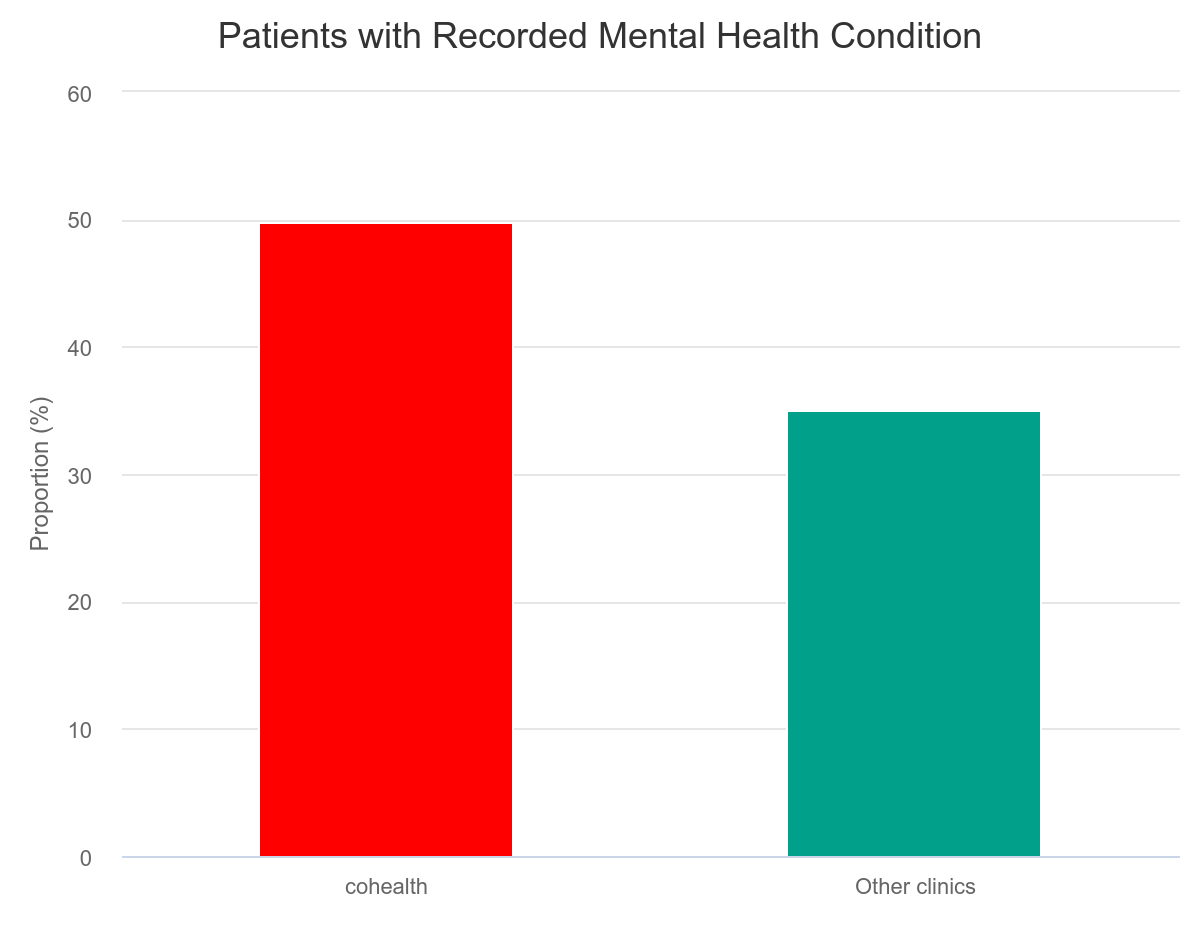
\includegraphics[width=0.45\linewidth,height=\textheight,keepaspectratio]{./images/patients-with-recorded-mentalhealth.png}
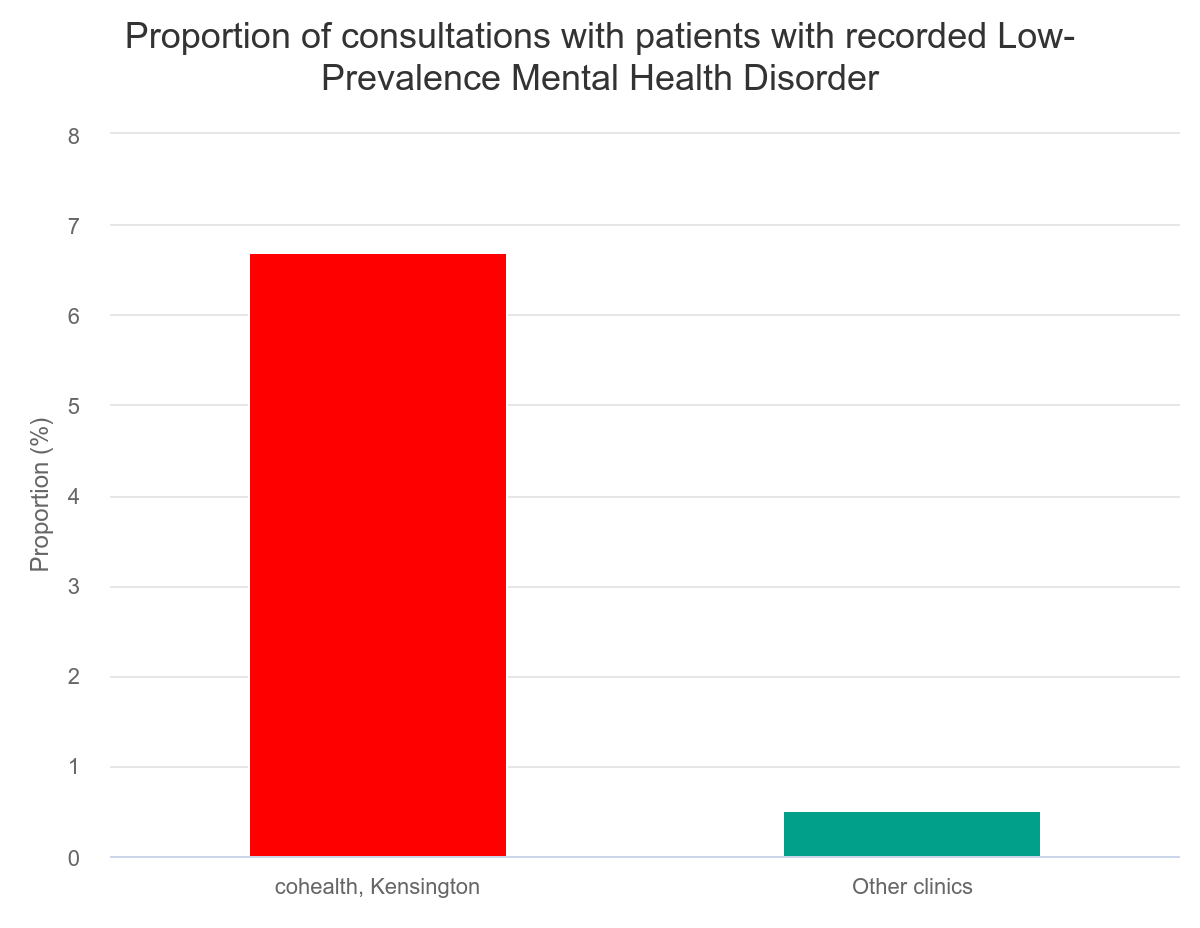
\includegraphics[width=0.45\linewidth,height=\textheight,keepaspectratio]{./images/proportion-of-consultation-lowprevalence.png}\end{minipage}%

\end{figure}%

}

\caption{\label{figure-mhtpdcp}Prevalence of mental health conditions at
cohealth general practice clinics}

\end{figure}%

To encourage general practitioners to provide a structured framework for
assessing, managing and coordinating the mental health care of patients
with mental health conditions, the Medicare Benefits Schedule (MBS)
provides reimbursement for general practitioners to write (and bill) `GP
Mental Health Treatment Plans (MHTPs)'. The preparation and billing of a
mental health treatment plan also enables a patient to access Medicare
rebates for private psychological services\sidenote{\footnotesize \href{https://gpmhsc.org.au/info/detail/11920366-5b75-449e-9503-e8143478817b/why-do-mental-health-treatment-plans}{General
  Practitioner Mental Health Standards Collaboration - `What is a mental
  health treatment plan?'}}. A secondary use of MHTP item billing, and
billing of the
\href{https://www9.health.gov.au/mbs/fullDisplay.cfm?type=item&q=2713}{mental
health treatment plan `review' item 2712}, is as a - perhaps misleading
- indicator of mental health services delivered in general
practice\sidenote{\footnotesize ``\href{https://www1.racgp.org.au/newsgp/professional/gps-rebut-criticism-of-mental-health-care-plan-ove}{GPs
  rebut criticism of mental health care plan oversight}''. Joyon
  Attwooll, RACGP newsGP, 8 August 2022.} \sidenote{\footnotesize ``\href{https://insightplus.mja.com.au/2022/30/myth-busting-role-of-the-gp-in-primary-mental-health-care/}{Myth-busting:
  role of the GP in primary mental health care}''. Louise Stone, Karen
  Spielman, Michael Tam, Johanna Lynch, May Su, Tim Senior, Karen Price,
  Sarah Chalmers, Gwendoline Burton. MJA Insight+, 8 August 2022.}
\sidenote{\footnotesize ``\href{https://insightplus.mja.com.au/2022/28/access-to-primary-mental-health-care-remains-critical/}{Access
  to primary mental health care remains critical}''. Sebastian
  Rosenberg, Ian Hickie. MJA Insight+, 25 July 2022.}.

Although cohealth consults a high proportion of patients with recorded
mental health conditions and are potentially eligible for mental health
treatment plans (MHTP), a relatively small proportion of those patients
have had - and been billed - an `up-to-date' treatment plan i.e.~within
the past twelve months. At cohealth, 15.5\% of eligible patients have an
up-to-date treatment plan, compared to 21.3\% nationally (see
Section~\ref{sec-appendix-mhtpeligible}). The proportion of all patients
at cohealth who have an up-to-date mental health treatment plan (7.7\%)
is almost indistinguishable from the proportion of other clinics
(7.5\%).

\begin{Shaded}
\begin{Highlighting}[]
\CommentTok{\# Data for the first plot}
\CommentTok{\# patients eligible for MHTP who have an up{-}to{-}date MHTP}
\NormalTok{df1 }\OtherTok{\textless{}{-}} \FunctionTok{data.frame}\NormalTok{(}
  \AttributeTok{Clinic =} \FunctionTok{c}\NormalTok{(}\StringTok{"cohealth"}\NormalTok{, }\StringTok{"Other clinics"}\NormalTok{),}
  \AttributeTok{Percentage =} \FunctionTok{c}\NormalTok{(}
    \FunctionTok{round}\NormalTok{(n\_mhtp\_cohealth}\SpecialCharTok{/}\NormalTok{n\_mentalhealth\_cohealth }\SpecialCharTok{*} \DecValTok{100}\NormalTok{, }\DecValTok{1}\NormalTok{),}
    \FunctionTok{round}\NormalTok{(n\_mhtp\_other}\SpecialCharTok{/}\NormalTok{n\_mentalhealth\_other }\SpecialCharTok{*} \DecValTok{100}\NormalTok{, }\DecValTok{1}\NormalTok{)}
\NormalTok{  )}
\NormalTok{)}

\CommentTok{\# Data for the second plot}
\CommentTok{\# all patients, proportion who have an up{-}to{-}date MHTP}
\NormalTok{df2 }\OtherTok{\textless{}{-}} \FunctionTok{data.frame}\NormalTok{(}
  \AttributeTok{Clinic =} \FunctionTok{c}\NormalTok{(}\StringTok{"cohealth"}\NormalTok{, }\StringTok{"Other clinics"}\NormalTok{),}
  \AttributeTok{Percentage =} \FunctionTok{c}\NormalTok{(}
    \FunctionTok{round}\NormalTok{(n\_mhtp\_cohealth}\SpecialCharTok{/}\NormalTok{n\_total\_cohealth }\SpecialCharTok{*} \DecValTok{100}\NormalTok{, }\DecValTok{1}\NormalTok{),}
    \FunctionTok{round}\NormalTok{(n\_mhtp\_other}\SpecialCharTok{/}\NormalTok{n\_total\_other }\SpecialCharTok{*} \DecValTok{100}\NormalTok{, }\DecValTok{1}\NormalTok{)}
\NormalTok{  )}
\NormalTok{)}

\CommentTok{\# Choose a Wes Anderson palette (e.g., \textquotesingle{}Rushmore\textquotesingle{})}
\NormalTok{palette }\OtherTok{\textless{}{-}} \FunctionTok{wes\_palette}\NormalTok{(}\StringTok{"Darjeeling1"}\NormalTok{, }\DecValTok{2}\NormalTok{, }\AttributeTok{type =} \StringTok{"discrete"}\NormalTok{)}

\NormalTok{hc1 }\OtherTok{\textless{}{-}} \FunctionTok{highchart}\NormalTok{() }\SpecialCharTok{|\textgreater{}}
  \FunctionTok{hc\_chart}\NormalTok{(}\AttributeTok{type =} \StringTok{"bar"}\NormalTok{) }\SpecialCharTok{|\textgreater{}}
  \FunctionTok{hc\_title}\NormalTok{(}\AttributeTok{text =} \StringTok{"Eligible patients with an up{-}to{-}date mental health treatment plan (MHTP)"}\NormalTok{) }\SpecialCharTok{|\textgreater{}}
  \FunctionTok{hc\_xAxis}\NormalTok{(}\AttributeTok{categories =}\NormalTok{ df1}\SpecialCharTok{$}\NormalTok{Clinic) }\SpecialCharTok{|\textgreater{}}
  \FunctionTok{hc\_yAxis}\NormalTok{(}\AttributeTok{title =} \FunctionTok{list}\NormalTok{(}\AttributeTok{text =} \StringTok{"Proportion (\%)"}\NormalTok{)) }\SpecialCharTok{|\textgreater{}}
  \FunctionTok{hc\_add\_series}\NormalTok{(}
    \AttributeTok{name =} \StringTok{"Proportion"}\NormalTok{,}
    \AttributeTok{data =}\NormalTok{ df1}\SpecialCharTok{$}\NormalTok{Percentage,}
    \AttributeTok{colorByPoint =} \ConstantTok{TRUE}\NormalTok{,}
    \AttributeTok{colors =}\NormalTok{ palette}
\NormalTok{  ) }\SpecialCharTok{|\textgreater{}}
  \FunctionTok{hc\_tooltip}\NormalTok{(}\AttributeTok{pointFormat =} \StringTok{"\textless{}b\textgreater{}\{point.y\}\%\textless{}/b\textgreater{}"}\NormalTok{) }\SpecialCharTok{|\textgreater{}}
  \FunctionTok{hc\_legend}\NormalTok{(}\AttributeTok{enabled =} \ConstantTok{FALSE}\NormalTok{) }\SpecialCharTok{|\textgreater{}}
  \FunctionTok{hc\_exporting}\NormalTok{(}\AttributeTok{enabled =} \ConstantTok{TRUE}\NormalTok{)}

\CommentTok{\# Second highcharter plot}
\NormalTok{hc2 }\OtherTok{\textless{}{-}} \FunctionTok{highchart}\NormalTok{() }\SpecialCharTok{|\textgreater{}}
  \FunctionTok{hc\_chart}\NormalTok{(}\AttributeTok{type =} \StringTok{"bar"}\NormalTok{) }\SpecialCharTok{|\textgreater{}}
  \FunctionTok{hc\_title}\NormalTok{(}\AttributeTok{text =} \StringTok{"Proportion of all patients with an up{-}to{-}date mental health treatment plan (MHTP)"}\NormalTok{) }\SpecialCharTok{|\textgreater{}}
  \FunctionTok{hc\_xAxis}\NormalTok{(}\AttributeTok{categories =}\NormalTok{ df2}\SpecialCharTok{$}\NormalTok{Clinic) }\SpecialCharTok{|\textgreater{}}
  \FunctionTok{hc\_yAxis}\NormalTok{(}\AttributeTok{title =} \FunctionTok{list}\NormalTok{(}\AttributeTok{text =} \StringTok{"Proportion (\%)"}\NormalTok{)) }\SpecialCharTok{|\textgreater{}}
  \FunctionTok{hc\_add\_series}\NormalTok{(}
    \AttributeTok{name =} \StringTok{"Proportion"}\NormalTok{,}
    \AttributeTok{data =}\NormalTok{ df2}\SpecialCharTok{$}\NormalTok{Percentage,}
    \AttributeTok{colorByPoint =} \ConstantTok{TRUE}\NormalTok{,}
    \AttributeTok{colors =}\NormalTok{ palette}
\NormalTok{  ) }\SpecialCharTok{|\textgreater{}}
  \FunctionTok{hc\_tooltip}\NormalTok{(}\AttributeTok{pointFormat =} \StringTok{"\textless{}b\textgreater{}\{point.y\}\%\textless{}/b\textgreater{}"}\NormalTok{) }\SpecialCharTok{|\textgreater{}}
  \FunctionTok{hc\_legend}\NormalTok{(}\AttributeTok{enabled =} \ConstantTok{FALSE}\NormalTok{) }\SpecialCharTok{|\textgreater{}}
  \FunctionTok{hc\_exporting}\NormalTok{(}\AttributeTok{enabled =} \ConstantTok{TRUE}\NormalTok{)}
\end{Highlighting}
\end{Shaded}

\begin{figure}

\centering{

\begin{figure}[H]

\begin{minipage}{0.50\linewidth}
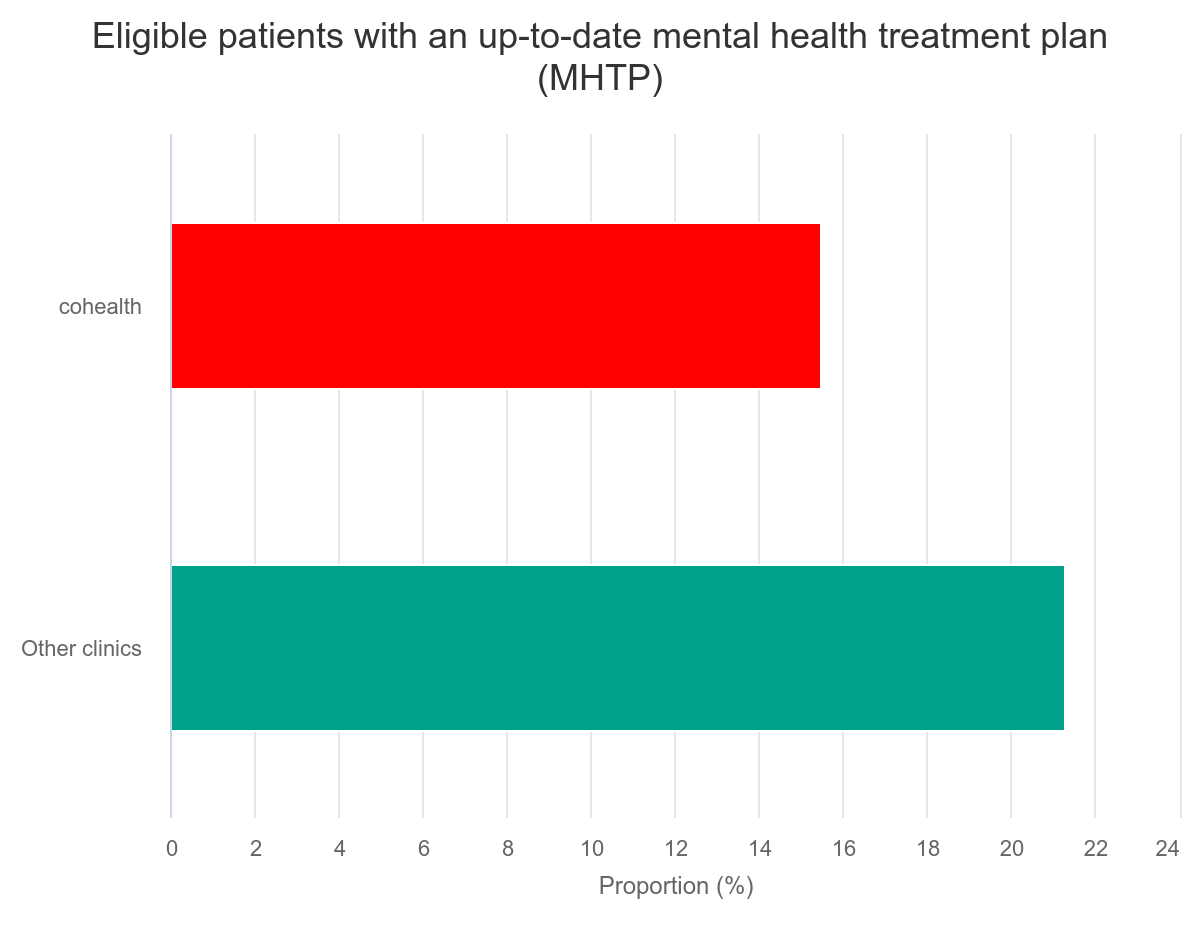
\includegraphics[width=0.45\linewidth,height=\textheight,keepaspectratio]{./images/eligible-patients-with-mhtp.png}
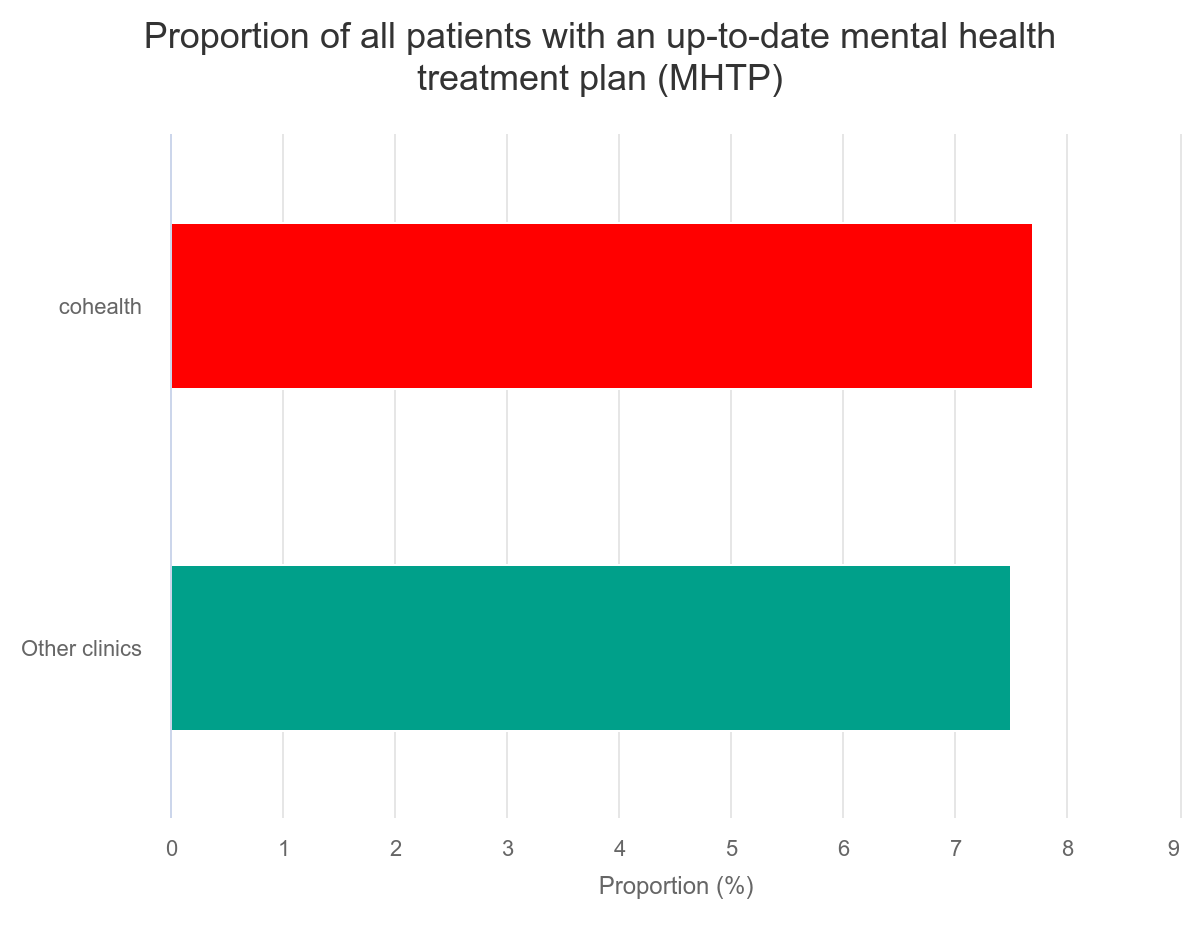
\includegraphics[width=0.45\linewidth,height=\textheight,keepaspectratio]{./images/active-patients-with-mhtp.png}\end{minipage}%

\end{figure}%

}

\caption{\label{figure-mhtp_dcp}cohealth general practice clinics usage
of mental health treatment plans (MHTPs)}

\end{figure}%

\subsection{The problem with Mental Health Treatment Plans
(MHTP)}\label{the-problem-with-mental-health-treatment-plans-mhtp}

Why, despite the high prevalence of mental health conditions among
cohealth clinic patients, do cohealth general practice clinics do - and
bill - relatively few mental health treatment plans (MHTPs)?

cohealth general practitioners suggested the following reasons, broadly
summarised as:

\begin{itemize}
\tightlist
\item
  Some patients benefit more from mental health treatment plans than
  others.
\item
  Patients at cohealth, particularly those with lower socio-economic
  resources, might not benefit from mental health treatment plans as
  much as patients with financial resources to pay for private
  psychological services.
\item
  Mental health treatment plans are cumbersome to prepare, particularly
  if the patient does not particularly benefit the preparation of a
  mental health treatment plan.
\item
  Patients with lower socio-economic resources or more severe mental
  health illness might have generally lower access to care. This
  includes access to third-party services, and might even include access
  to cohealth general practice (primary care) and other services.
\end{itemize}

In detail:

\begin{enumerate}
\def\labelenumi{\arabic{enumi}.}
\item
  Mental health treatment plans are done principally for patients to
  access private psychological services.

  \begin{enumerate}
  \def\labelenumii{\roman{enumii})}
  \tightlist
  \item
    Some patients with mental health conditions can access at least some
    psychological and psychiatric services through mechanisms which do
    not require a mental health treatment plan. Examples of services
    which are accessible without a mental health treatment plan are:

    \begin{enumerate}
    \def\labelenumiii{\alph{enumiii}.}
    \tightlist
    \item
      The area mental health service (e.g.~patients living with
      schizophrenia and being prescribed clozapine)
    \item
      The \href{https://www.ndis.gov.au/}{National Disability Insurance
      Scheme (NDIS)}, for
      \href{https://www.ndis.gov.au/media/112/download}{patients living
      with long-term disability resulting from their mental health
      condition}.
    \item
      Through the Primary Health Network's
      \href{https://nwmphn.org.au/our-work/mental-health/careinmind-mental-health-services/}{CAREinMIND},
      which does not currently require a mental health treatment plan
      for purposes of referral.
    \item
      Through cohealth's other counselling services (e.g.~provided by
      social workers).
    \end{enumerate}
  \item
    Paradoxically, patients who can have considerable disability as the
    result of a mental health condition (e.g.~schizophrenia, or
    qualifying for NDIS) may have less benefit from a mental health
    treatment plan, if the mental health treatment plan is primarily
    being used to help fund private psychological services.
  \end{enumerate}
\item
  As a result, mental health treatment plans are not equivalent to
  referral to psychological care for patients, as at least some patients
  with mental health conditions can receive psychological care through
  other funding sources.
\item
  A general-practitioner prepared (and billed) mental health
  care/treatment plan does
  \href{https://www.servicesaustralia.gov.au/mental-health-care-and-medicare?context=60092}{provide
  access to Medicare funding for private psychological services}.
  However, many private psychologists charge fees in excess of the
  Medicare rebate for psychological services, resulting in a large `gap'
  fee for patients\sidenote{\footnotesize ``\href{https://psychology.org.au/about-us/news-and-media/aps-in-the-media/2023/long-wait-times-$90-gap-fees-preventing-access-to}{Long
    wait times \$90 gap fees preventing access to psychology
    services''}'' Australian Psychological Society, 30 January 2023.}.

  The size of the `gap fee' is a potential barrier for some patients to
  access psychological services, particularly those from low
  socio-economic backgrounds. For patients who do not have the financial
  resources to pay the `gap fees' of private psychological care, the
  preparation of a general-practitioner mental health treatment plan
  could be of less value compared to a patient who is not deterred by
  the `gap fee' and is seeking Medicare subsidies for private
  psychological treatment.
\item
  The general practitioner may view the preparation of a mental health
  treatment plan to be of little use to the patient, particularly those
  who cannot afford to pay the `gap fee' of private psychological
  services. Although there is some financial return for the general
  practitioner to prepare a mental health treatment plan, the patient
  may have more pressing concerns e.g.~immediate counselling provided by
  the general practitioner, housing issues or addressing `physical'
  health needs.
\item
  Although universal health insurance in Australia and the frequent use
  of bulk-billing at cohealth clinics might reduce inequity in
  access\sidenote{\footnotesize ``\href{https://fac.flinders.edu.au/dspace/api/core/bitstreams/15a05634-bc77-4107-8582-69820927b6b5/content}{Socioeconomic
    status and accessibility to health care services in Australia}''. R
    Katteri, Research Roundup, Primary Health Care Research and
    Information Services (PHCRIS), Issue 22, December 2011.} for
  cohealth patients living with mental health illness and low
  socio-economic resources, there may still be inequity in services
  provided in relation to need.
\end{enumerate}

Some of the reasons listed can be tested through examination of practice
billing compared to patient characteristics:

\begin{itemize}
\tightlist
\item
  Are patients with mental health conditions and with fewer financial
  resources more or less likely to have a mental health treatment plan
  billed?

  \begin{itemize}
  \tightlist
  \item
    The patient's possession of a
    \href{https://www.servicesaustralia.gov.au/concession-and-health-care-cards?context=60091}{health
    concession or pension card} is potential proxy for less financial
    resources\sidenote{\footnotesize ``\href{https://www.racgp.org.au/getattachment/65163663-b9c2-4989-91b0-99bf3b317e6b/attachment.aspx\#:~:text=A\%20proxy\%20for\%20socioeconomic\%20status\%20is\%20entitlement,free\%20after\%20a\%20cost\%20threshold\%20is\%20reached.&text=Health\%20care\%20card\%20holders\%20were\%20more\%20likely,nomic\%20status\%20than\%20nonhealth\%20care\%20card\%20holders.}{GP
      visits by health care card holders (A secondary analysis of data
      from Bettering the Evaluation and Care of Health (BEACH), a
      national study of general practice activity in Australia)}''.
      Janice Charles, Lisa Valenti, Helena Britt. \emph{Australian
      Family Physician}, Vol 32: No.~1/2, pp 85-89. January/February
      2003.} \sidenote{\footnotesize ``\href{https://doi.org/10.1111/jpc.16450}{The
      impact of low socioeconomic status and primary health care access
      on emergency department presentations in young children in
      regional Queensland}''. Catherine McCosker, Gavin Beccaria, Lisa
      Beccaria, Tanya Machin. \emph{Journal of Paediatric and Child
      Health}, Vol 59:9, pp 1035-1038. September 2023.}.
  \end{itemize}
\item
  Are patients with higher-need mental health conditions,
  e.g.~low-prevalence disorders (schizophrenia and bipolar affective
  disorder) more or less likely to have a mental health treatment plan
  billed?
\item
  MHTPs may be perceived to have burdensome time and documentation
  requirements. Other mental health-related MBS service items may not
  have as burdensome time and documentation requirements as MHTPs. Are
  mental health MBS service items with less burdensome requirements more
  or less commonly used for patients with limited financial resources or
  those with low-prevalence mental health disorders?

  \begin{itemize}
  \tightlist
  \item
    One mental health-related MBS service item number is ``Professional
    attendance by a general practitioner in relation to a mental
    disorder and of at least 20 minutes in duration'' (MBS item 2713,
    full details can be found on
    \href{https://www9.health.gov.au/mbs/fullDisplay.cfm?type=item&q=2713}{MBS
    Online})
  \item
    Another group of relevant mental health-related MBS services are the
    focused psychological strategies (FPS) MBS service items (items
    2721, 2723, 2725 and 2727. More details can be found on the
    \href{https://gpmhsc.org.au/info/detail/56bb2adf-75b6-4d2e-97c0-85b6d0f295fd/level-2-focussed-psychological-strategies}{General
    Practice Mental Health Standards Collaboration} website). However,
    none of the practice sites (Kensington, Paisley St, Laverton,
    Fitzroy and Collingwood) had claimed any of the FPS MBS items in the
    year prior to 1 May 2025.
  \end{itemize}
\item
  If patients living with mental health conditions and low
  socio-economic resources or low-prevalence mental conditions have
  difficulty with access or provision of co-ordinated care from cohealth
  general practitioners, they might also receive less care planning for
  other (e.g.~physical) conditions.

  \begin{itemize}
  \tightlist
  \item
    People living with a mental health condition are, compared to the
    general population, more likely to to live with other co-existing
    physical conditions, including chronic and life-changing conditions
    such as cardiovascular disease, airways disease and diabetes. People
    living with mental health illness are also more likely to struggle
    with regular activities\sidenote{\footnotesize ``\href{https://www.equallywell.org.au/wp-content/uploads/2018/12/Equally-Well-National-Consensus-Booklet-47537.pdf}{Improving
      the physical health and wellbeing of people living with mental
      illness in Australia}'', National Mental Health Commission (NHMC),
      2016.}. Patient living with a mental health condition are more
    likely to require planning and coordination for health care needs
    (e.g.~diabetes) in addition to their mental health needs.
  \item
    To encourage general practitioners to plan and coordinate the health
    care of patients with ongoing chronic health conditions, the
    Medicare Benefits Schedule (MBS) provides reimbursement for general
    practitioners to write (and bill) `GP Chronic Disease and Management
    Plan (GPMP,
    \href{https://www9.health.gov.au/mbs/fullDisplay.cfm?type=item&q=721}{MBS
    item 721})\sidenote{\footnotesize ``\href{https://www.racgp.org.au/getattachment/b85620ff-5aa3-489a-b423-c667d142bca6/attachment.aspx}{General
      practice and the management of chronic conditions, Where to
      now?}'' (Jan Newland, Nicholas Zwar. \emph{Australian Family
      Physician}, Jan/Feb/2006, Vol 36:No 1-2, pp 16-19). Note that the
      \href{https://www1.racgp.org.au/newsgp/professional/full-details-of-incoming-cdm-changes-revealed}{chronic
      disease management item numbers in use as of May 2025 are
      scheduled to be changed on July 2025}.}'.
  \end{itemize}
\end{itemize}

\subsection{Method}\label{method}

\subsubsection{Mental health treatment
plans}\label{mental-health-treatment-plans}

\begin{itemize}
\item
  It is postulated that concession card holders have lower financial
  resources and are less able to utilise the government subsidies
  unlocked by MHTP plans for private psychology. This is because private
  psychology fees are often far greater than the government subsidy to
  use private psychology.
\item
  Mental health conditions can be broadly divided into low- and high-
  prevalence mental health conditions. High-prevalence mental health
  conditions are the common mental health conditions such as anxiety and
  depression. Low-prevalence mental health conditions are the less
  common, and often lifelong conditions, of schizophrenia and bipolar
  affective disorder. Low-prevalence mental health conditions often have
  a substantial impact on individuals and their family, requiring
  extensive support\sidenote{\footnotesize ``\href{https://www.aihw.gov.au/getmedia/1838295a-5588-4747-9515-b826a5ab3d5a/aihw-aus-221-chapter-3-12.pdf}{Australia's
    health 2018}'', Chapter 3.12, Mental Health. Australian Institute of
    Health and Welfare (AIHW), 2018.}. Patients with schizophrenia and
  bipolar affective disorder can benefit from psychological therapies.
  If mental health treatment plans were done on the basis of need, it
  would be expected that more patients with low-prevalence conditions
  would have mental health treatment plans compared to patients with
  high-prevalence mental health conditions.
\end{itemize}

\emph{Are concession card holders, or patients living with
low-prevalence mental health disorders, billed the mental health
treatment plans (MHTP) the same, more, or less than patients without
concession card holders at cohealth clinics?}

\subsubsection{Mental health consultation (MBS item
`2713')}\label{mental-health-consultation-mbs-item-2713}

If patients with mental health conditions \emph{and} a health concession
card have less mental health treatment plans billed at cohealth general
practices, perhaps those patients \emph{also} have less mental health
care delivered by those general practitioners.

There other potential ways to measure mental health care delivery in
general practice.

Potential measurements:

\begin{enumerate}
\def\labelenumi{\arabic{enumi}.}
\tightlist
\item
  Examination of `reasons for consult' in general practice electronic
  medical record (EMR) notes

  \begin{enumerate}
  \def\labelenumii{\roman{enumii})}
  \tightlist
  \item
    Relatively easy to do, as reasons for consult are part of
    `structured data' within the EMR
  \end{enumerate}
\item
  Examination of the electronic medical record (EMR) consultation notes

  \begin{enumerate}
  \def\labelenumii{\roman{enumii})}
  \tightlist
  \item
    More difficult to do than option (1), but can be done with basic
    natural language processing (NLP)
  \end{enumerate}
\item
  Examination of other billing items associated with mental health care
\end{enumerate}

Options (1) and (2) are relatively easy to perform with a basic database
search and simple application of data science. However, at the time of
writing, only option (3) is currently available to use at cohealth.

There \emph{is} another billing item associated with mental health care,
which is the
\href{https://www9.health.gov.au/mbs/fullDisplay.cfm?type=item&q=2713}{general
practitioner attendance in relation to a mental health disorder,
Medicare Benefit Schedule - Item 2713}. Unfortunately, MBS item 2713 is
little used, because there are alternative item numbers - not specific
to mental health - which are easy to use and bill\sidenote{\footnotesize \href{https://www9.health.gov.au/mbs/fullDisplay.cfm?type=item&q=2713}{MBS
  item 2713} has a requirement for minimum consultation length of 20
  minutes, and has a rebate value of \$81.70.
  \endgraf
  There is an alternative item number which can also be claimed if a
  consult is between 20 to 40 minutes in length, the level `C' consult,
  \href{https://www9.health.gov.au/mbs/fullDisplay.cfm?type=item&q=36&qt=item}{MBS
  item 36}, which has a rebate value of \$82.90. Where an item 2713
  could be claimed, an item 36 could be claimed instead, with greater
  revenue than an item 2713.
  \endgraf
  This is even more the case when a patient has a concession card. In
  that case, the bulk-billing incentive payment for item 36 is \$14 or
  more (depending on the practice's country-rural `MMM' location) than
  the bulk-biling incentive payment for an item 2713.}.

Nevertheless, occasionally general practitioners \emph{do} claim an item
2713\sidenote{\footnotesize One possible reason a 2713 is billed, despite the
  relatively low financial return compared to an `item C', is because
  item 2713 - depending on the duration and content of the consult - can
  sometimes be `co-billed' together with a standard consult item (such
  as level B or C consult).}.

\emph{Are concession card holders, or patients living with
low-prevalence mental health disorders, billed the general practice
mental health item `MBS Item 2713' the same, more, or less than patients
without concession card holders at cohealth clinics?}

\subsubsection{Chronic disease management plans (MBS item
`721')}\label{chronic-disease-management-plans-mbs-item-721}

Another indicator of care provision is the billing of
\href{https://www9.health.gov.au/mbs/fullDisplay.cfm?type=item&q=721}{general
practitioner chronic disease management plans, Medicare Benefit Schedule
item 721}. Chronic disease management plans are for the purpose of
planning, setting goals, coordinating and reviewing an ongoing chronic
condition (present for more than six months or expected to be present
for more than six months). People living with mental health conditions,
particularly low-prevalence mental health conditions and those living
with socio-economic disadvantage are more likely to live with chronic
health conditions and experience disability as the result of those
conditions.

\emph{Are concession card holders, or patients living with
low-prevalence mental health disorders, billed chronic disease
management plans `MBS item 721' the same, more, or less than patients
without concession card holders at cohealth clinics?}

\subsubsection{Data gathering and
analysis}\label{data-gathering-and-analysis}

The number of active patients at coHealth living with mental health
conditions, who were billed MHTPs, mental health consult items (MBS item
2713) or chronic disease management plans (MBS item 721) in the previous
twelve months (up to 1st May 2025) were counted using PenCS (for details
of the extraction procedure using PenCS, see
Section~\ref{sec-appendix-mhtpgroups}). The patients were divided into
groups according to concession card holder patients (either health care
card `HCC' or pension card), high-prevalence and low-prevalence mental
health disorders and the cohealth clinic site attended.

The results are analysed using \href{https://www.r-project.org/}{R
version 4.3.1}. Logistic regression was used, with clinic location as a
random effect\sidenote{\footnotesize It is to be noted that using clinic location as a
  random effect added little information to the model.}. Clinic location
was used as a random effect because clinicians, support staff
(e.g.~mental health nurses) availability, and potentially workplace
cultures are expected to be different at each clinic site. Some clinic
sites are relatively close together geographically, but other sites are
located in geographically distinct communities.

Source code can be viewed on www.github.com/DavidPatShuiFong\sidenote{\footnotesize \href{https://github.com/DavidPatShuiFong/vkelimHomepage/tree/master/static/post/mhtpdisadvantage}{R
  source code on Github}} and davidfong.org\sidenote{\footnotesize \href{https://www.davidfong.org/post/mhtpdisadvantage/}{R
  source code `inline' on davidfong.org}}.

\subsection{Results}\label{results}

\begin{Shaded}
\begin{Highlighting}[]
\CommentTok{\# outcome}
\CommentTok{\#   counts of patients who have had, in the past year:}
\CommentTok{\#     mhtp{-} mental health treatment plan e.g. MBS item 2715, 2717}
\CommentTok{\#     mh2713 {-} general practitioner mental health consult i.e. MBS item 2713}
\CommentTok{\#     gpmp {-} general practitioenr chronic disease treatment plan i.e. MBS item 721}
\CommentTok{\# }
\CommentTok{\# predictors}
\CommentTok{\#   concession {-} false = no, true = yes}
\CommentTok{\#   mental health condition {-} "high" = high{-}prevalence, "low" = low{-}prevalence}
\CommentTok{\# }
\CommentTok{\# random effects}
\CommentTok{\#   (not considered to be a predictor of interest)}
\CommentTok{\#   clinic {-} the clinic\textquotesingle{}s name, a categorical variable}

\CommentTok{\# the initial data was created as counts (i.e. aggregated data)}
\CommentTok{\# the original patient data can be recreated from the counts}

\NormalTok{summary\_df }\OtherTok{\textless{}{-}} \FunctionTok{tibble}\NormalTok{(}
  \AttributeTok{concession =} \FunctionTok{logical}\NormalTok{(),}
  \AttributeTok{condition =} \FunctionTok{factor}\NormalTok{(),}
  \AttributeTok{clinic =} \FunctionTok{character}\NormalTok{(),}
  \AttributeTok{total =} \FunctionTok{integer}\NormalTok{(), }\CommentTok{\# number in this patient category (concession, condition, clinic) occurs}
  \AttributeTok{mhtp =} \FunctionTok{integer}\NormalTok{(), }\CommentTok{\# number who had a mental health treatment plan (MHTP e.g. 2715/2717)}
  \AttributeTok{mh2713 =} \FunctionTok{integer}\NormalTok{(), }\CommentTok{\# number who had a billed GP mental health consult (MBS item 2713)}
  \AttributeTok{gpmp =} \FunctionTok{integer}\NormalTok{() }\CommentTok{\# number who had a chronic disease management plan (MBS item 721)}
\NormalTok{)}

\NormalTok{summary\_df }\OtherTok{\textless{}{-}}\NormalTok{ summary\_df }\SpecialCharTok{|\textgreater{}}
  \FunctionTok{add\_row}\NormalTok{(}\AttributeTok{concession =} \ConstantTok{TRUE}\NormalTok{, }\AttributeTok{condition =} \StringTok{"high"}\NormalTok{, }\AttributeTok{clinic =} \StringTok{"Kensington"}\NormalTok{, }\AttributeTok{total =} \DecValTok{285}\NormalTok{, }\AttributeTok{mhtp =} \DecValTok{42}\NormalTok{, }\AttributeTok{mh2713 =} \DecValTok{13}\NormalTok{, }\AttributeTok{gpmp =} \DecValTok{109}\NormalTok{) }\SpecialCharTok{|\textgreater{}}
  \FunctionTok{add\_row}\NormalTok{(}\AttributeTok{concession =} \ConstantTok{TRUE}\NormalTok{, }\AttributeTok{condition =} \StringTok{"low"}\NormalTok{, }\AttributeTok{clinic =} \StringTok{"Kensington"}\NormalTok{, }\AttributeTok{total =} \DecValTok{73}\NormalTok{, }\AttributeTok{mhtp =} \DecValTok{7}\NormalTok{, }\AttributeTok{mh2713 =} \DecValTok{7}\NormalTok{, }\AttributeTok{gpmp =} \DecValTok{33}\NormalTok{) }\SpecialCharTok{|\textgreater{}}
  \FunctionTok{add\_row}\NormalTok{(}\AttributeTok{concession =} \ConstantTok{FALSE}\NormalTok{, }\AttributeTok{condition =} \StringTok{"high"}\NormalTok{, }\AttributeTok{clinic =} \StringTok{"Kensington"}\NormalTok{, }\AttributeTok{total =} \DecValTok{84}\NormalTok{, }\AttributeTok{mhtp =} \DecValTok{9}\NormalTok{, }\AttributeTok{mh2713 =} \DecValTok{4}\NormalTok{, }\AttributeTok{gpmp =} \DecValTok{19}\NormalTok{) }\SpecialCharTok{|\textgreater{}}
  \FunctionTok{add\_row}\NormalTok{(}\AttributeTok{concession =} \ConstantTok{FALSE}\NormalTok{, }\AttributeTok{condition =} \StringTok{"low"}\NormalTok{, }\AttributeTok{clinic =} \StringTok{"Kensington"}\NormalTok{, }\AttributeTok{total =} \DecValTok{8}\NormalTok{, }\AttributeTok{mhtp =} \DecValTok{2}\NormalTok{, }\AttributeTok{mh2713 =} \DecValTok{0}\NormalTok{, }\AttributeTok{gpmp =} \DecValTok{3}\NormalTok{) }\SpecialCharTok{|\textgreater{}}
  \FunctionTok{add\_row}\NormalTok{(}\AttributeTok{concession =} \ConstantTok{TRUE}\NormalTok{, }\AttributeTok{condition =} \StringTok{"high"}\NormalTok{, }\AttributeTok{clinic =} \StringTok{"Paisley"}\NormalTok{, }\AttributeTok{total =} \DecValTok{430}\NormalTok{, }\AttributeTok{mhtp =} \DecValTok{26}\NormalTok{, }\AttributeTok{mh2713 =} \DecValTok{42}\NormalTok{, }\AttributeTok{gpmp =} \DecValTok{164}\NormalTok{) }\SpecialCharTok{|\textgreater{}}
  \FunctionTok{add\_row}\NormalTok{(}\AttributeTok{concession =} \ConstantTok{TRUE}\NormalTok{, }\AttributeTok{condition =} \StringTok{"low"}\NormalTok{, }\AttributeTok{clinic =} \StringTok{"Paisley"}\NormalTok{, }\AttributeTok{total =} \DecValTok{123}\NormalTok{, }\AttributeTok{mhtp =} \DecValTok{13}\NormalTok{, }\AttributeTok{mh2713 =} \DecValTok{10}\NormalTok{, }\AttributeTok{gpmp =} \DecValTok{58}\NormalTok{) }\SpecialCharTok{|\textgreater{}}
  \FunctionTok{add\_row}\NormalTok{(}\AttributeTok{concession =} \ConstantTok{FALSE}\NormalTok{, }\AttributeTok{condition =} \StringTok{"high"}\NormalTok{, }\AttributeTok{clinic =} \StringTok{"Paisley"}\NormalTok{, }\AttributeTok{total =} \DecValTok{131}\NormalTok{, }\AttributeTok{mhtp =} \DecValTok{21}\NormalTok{, }\AttributeTok{mh2713 =} \DecValTok{14}\NormalTok{, }\AttributeTok{gpmp =} \DecValTok{26}\NormalTok{) }\SpecialCharTok{|\textgreater{}}
  \FunctionTok{add\_row}\NormalTok{(}\AttributeTok{concession =} \ConstantTok{FALSE}\NormalTok{, }\AttributeTok{condition =} \StringTok{"low"}\NormalTok{, }\AttributeTok{clinic =} \StringTok{"Paisley"}\NormalTok{, }\AttributeTok{total =} \DecValTok{8}\NormalTok{, }\AttributeTok{mhtp =} \DecValTok{1}\NormalTok{, }\AttributeTok{mh2713 =} \DecValTok{0}\NormalTok{, }\AttributeTok{gpmp =} \DecValTok{4}\NormalTok{) }\SpecialCharTok{|\textgreater{}}
  \FunctionTok{add\_row}\NormalTok{(}\AttributeTok{concession =} \ConstantTok{TRUE}\NormalTok{, }\AttributeTok{condition =} \StringTok{"high"}\NormalTok{, }\AttributeTok{clinic =} \StringTok{"Laverton"}\NormalTok{, }\AttributeTok{total =} \DecValTok{79}\NormalTok{, }\AttributeTok{mhtp =} \DecValTok{14}\NormalTok{, }\AttributeTok{mh2713 =} \DecValTok{6}\NormalTok{, }\AttributeTok{gpmp =} \DecValTok{32}\NormalTok{) }\SpecialCharTok{|\textgreater{}}
  \FunctionTok{add\_row}\NormalTok{(}\AttributeTok{concession =} \ConstantTok{TRUE}\NormalTok{, }\AttributeTok{condition =} \StringTok{"low"}\NormalTok{, }\AttributeTok{clinic =} \StringTok{"Laverton"}\NormalTok{, }\AttributeTok{total =} \DecValTok{38}\NormalTok{, }\AttributeTok{mhtp =} \DecValTok{10}\NormalTok{, }\AttributeTok{mh2713 =} \DecValTok{15}\NormalTok{, }\AttributeTok{gpmp =} \DecValTok{18}\NormalTok{) }\SpecialCharTok{|\textgreater{}}
  \FunctionTok{add\_row}\NormalTok{(}\AttributeTok{concession =} \ConstantTok{FALSE}\NormalTok{, }\AttributeTok{condition =} \StringTok{"high"}\NormalTok{, }\AttributeTok{clinic =} \StringTok{"Laverton"}\NormalTok{, }\AttributeTok{total =} \DecValTok{43}\NormalTok{, }\AttributeTok{mhtp =} \DecValTok{7}\NormalTok{, }\AttributeTok{mh2713 =} \DecValTok{1}\NormalTok{, }\AttributeTok{gpmp =} \DecValTok{16}\NormalTok{) }\SpecialCharTok{|\textgreater{}}
  \FunctionTok{add\_row}\NormalTok{(}\AttributeTok{concession =} \ConstantTok{FALSE}\NormalTok{, }\AttributeTok{condition =} \StringTok{"low"}\NormalTok{, }\AttributeTok{clinic =} \StringTok{"Laverton"}\NormalTok{, }\AttributeTok{total =} \DecValTok{4}\NormalTok{, }\AttributeTok{mhtp =} \DecValTok{1}\NormalTok{, }\AttributeTok{mh2713 =} \DecValTok{1}\NormalTok{, }\AttributeTok{gpmp =} \DecValTok{1}\NormalTok{) }\SpecialCharTok{|\textgreater{}}
  \FunctionTok{add\_row}\NormalTok{(}\AttributeTok{concession =} \ConstantTok{TRUE}\NormalTok{, }\AttributeTok{condition =} \StringTok{"high"}\NormalTok{, }\AttributeTok{clinic =} \StringTok{"Collingwood"}\NormalTok{, }\AttributeTok{total =} \DecValTok{346}\NormalTok{, }\AttributeTok{mhtp =} \DecValTok{35}\NormalTok{, }\AttributeTok{mh2713 =} \DecValTok{17}\NormalTok{, }\AttributeTok{gpmp =} \DecValTok{88}\NormalTok{) }\SpecialCharTok{|\textgreater{}}
  \FunctionTok{add\_row}\NormalTok{(}\AttributeTok{concession =} \ConstantTok{TRUE}\NormalTok{, }\AttributeTok{condition =} \StringTok{"low"}\NormalTok{, }\AttributeTok{clinic =} \StringTok{"Collingwood"}\NormalTok{, }\AttributeTok{total =} \DecValTok{87}\NormalTok{, }\AttributeTok{mhtp =} \DecValTok{5}\NormalTok{, }\AttributeTok{mh2713 =} \DecValTok{10}\NormalTok{, }\AttributeTok{gpmp =} \DecValTok{20}\NormalTok{) }\SpecialCharTok{|\textgreater{}}
  \FunctionTok{add\_row}\NormalTok{(}\AttributeTok{concession =} \ConstantTok{FALSE}\NormalTok{, }\AttributeTok{condition =} \StringTok{"high"}\NormalTok{, }\AttributeTok{clinic =} \StringTok{"Collingwood"}\NormalTok{, }\AttributeTok{total =} \DecValTok{88}\NormalTok{, }\AttributeTok{mhtp =} \DecValTok{14}\NormalTok{, }\AttributeTok{mh2713 =} \DecValTok{4}\NormalTok{, }\AttributeTok{gpmp =} \DecValTok{17}\NormalTok{) }\SpecialCharTok{|\textgreater{}}
  \FunctionTok{add\_row}\NormalTok{(}\AttributeTok{concession =} \ConstantTok{FALSE}\NormalTok{, }\AttributeTok{condition =} \StringTok{"low"}\NormalTok{, }\AttributeTok{clinic =} \StringTok{"Collingwood"}\NormalTok{, }\AttributeTok{total =} \DecValTok{6}\NormalTok{, }\AttributeTok{mhtp =} \DecValTok{1}\NormalTok{, }\AttributeTok{mh2713 =} \DecValTok{0}\NormalTok{, }\AttributeTok{gpmp =} \DecValTok{1}\NormalTok{) }\SpecialCharTok{|\textgreater{}}
  \FunctionTok{add\_row}\NormalTok{(}\AttributeTok{concession =} \ConstantTok{TRUE}\NormalTok{, }\AttributeTok{condition =} \StringTok{"high"}\NormalTok{, }\AttributeTok{clinic =} \StringTok{"Fitzroy"}\NormalTok{, }\AttributeTok{total =} \DecValTok{445}\NormalTok{, }\AttributeTok{mhtp =} \DecValTok{74}\NormalTok{, }\AttributeTok{mh2713 =} \DecValTok{29}\NormalTok{, }\AttributeTok{gpmp =} \DecValTok{94}\NormalTok{) }\SpecialCharTok{|\textgreater{}}
  \FunctionTok{add\_row}\NormalTok{(}\AttributeTok{concession =} \ConstantTok{TRUE}\NormalTok{, }\AttributeTok{condition =} \StringTok{"low"}\NormalTok{, }\AttributeTok{clinic =} \StringTok{"Fitzroy"}\NormalTok{, }\AttributeTok{total =} \DecValTok{165}\NormalTok{, }\AttributeTok{mhtp =} \DecValTok{18}\NormalTok{, }\AttributeTok{mh2713 =} \DecValTok{13}\NormalTok{, }\AttributeTok{gpmp =} \DecValTok{38}\NormalTok{) }\SpecialCharTok{|\textgreater{}}
  \FunctionTok{add\_row}\NormalTok{(}\AttributeTok{concession =} \ConstantTok{FALSE}\NormalTok{, }\AttributeTok{condition =} \StringTok{"high"}\NormalTok{, }\AttributeTok{clinic =} \StringTok{"Fitzroy"}\NormalTok{, }\AttributeTok{total =} \DecValTok{91}\NormalTok{, }\AttributeTok{mhtp =} \DecValTok{20}\NormalTok{, }\AttributeTok{mh2713 =} \DecValTok{2}\NormalTok{, }\AttributeTok{gpmp =} \DecValTok{14}\NormalTok{) }\SpecialCharTok{|\textgreater{}}
  \FunctionTok{add\_row}\NormalTok{(}\AttributeTok{concession =} \ConstantTok{FALSE}\NormalTok{, }\AttributeTok{condition =} \StringTok{"low"}\NormalTok{, }\AttributeTok{clinic =} \StringTok{"Fitzroy"}\NormalTok{, }\AttributeTok{total =} \DecValTok{10}\NormalTok{, }\AttributeTok{mhtp =} \DecValTok{3}\NormalTok{, }\AttributeTok{mh2713 =} \DecValTok{1}\NormalTok{, }\AttributeTok{gpmp =} \DecValTok{1}\NormalTok{)}
\end{Highlighting}
\end{Shaded}

\begin{Shaded}
\begin{Highlighting}[]
\CommentTok{\# duplicate rows according to the weighting \textquotesingle{}mhtp\textquotesingle{},}
\CommentTok{\# hence "re{-}creating" the original patient{-}level data from the counts}
\NormalTok{mhtp }\OtherTok{\textless{}{-}}\NormalTok{ summary\_df }\SpecialCharTok{|\textgreater{}}
  \CommentTok{\# duplicate rows by number of mental health treatment plans (mhtp)}
  \FunctionTok{uncount}\NormalTok{(mhtp) }\SpecialCharTok{|\textgreater{}}
  \CommentTok{\# add back mhtp column to a logical}
  \FunctionTok{mutate}\NormalTok{(}\AttributeTok{mhtp =} \ConstantTok{TRUE}\NormalTok{) }\SpecialCharTok{|\textgreater{}} 
  \CommentTok{\# don\textquotesingle{}t need \textquotesingle{}total\textquotesingle{} column any more}
  \FunctionTok{select}\NormalTok{(concession, condition, clinic, mhtp) }\SpecialCharTok{|\textgreater{}}
  \FunctionTok{bind\_rows}\NormalTok{(}
    \CommentTok{\# do the same, except}
    \CommentTok{\# now duplicate rows by number who do not have mental health treatment plans}
\NormalTok{    summary\_df }\SpecialCharTok{|\textgreater{}}
      \FunctionTok{mutate}\NormalTok{(}\AttributeTok{no\_mhtp =}\NormalTok{ total }\SpecialCharTok{{-}}\NormalTok{ mhtp) }\SpecialCharTok{|\textgreater{}}
      \FunctionTok{uncount}\NormalTok{(no\_mhtp) }\SpecialCharTok{|\textgreater{}}
      \FunctionTok{mutate}\NormalTok{(}\AttributeTok{mhtp =} \ConstantTok{FALSE}\NormalTok{) }\SpecialCharTok{|\textgreater{}}
      \FunctionTok{select}\NormalTok{(concession, condition, clinic, mhtp)}
\NormalTok{  ) }\SpecialCharTok{|\textgreater{}}
  \FunctionTok{arrange}\NormalTok{(clinic, concession, condition)}
  
\FunctionTok{label}\NormalTok{(mhtp}\SpecialCharTok{$}\NormalTok{mhtp) }\OtherTok{=} \StringTok{"Mental Health Plan"}
\FunctionTok{label}\NormalTok{(mhtp}\SpecialCharTok{$}\NormalTok{concession) }\OtherTok{=} \StringTok{"Concession card"}
\FunctionTok{label}\NormalTok{(mhtp}\SpecialCharTok{$}\NormalTok{condition) }\OtherTok{=} \StringTok{"condition"}

\CommentTok{\# the basic model}
\NormalTok{model\_mhtp }\OtherTok{\textless{}{-}} \FunctionTok{glm}\NormalTok{(}
\NormalTok{  mhtp }\SpecialCharTok{\textasciitilde{}}\NormalTok{ concession }\SpecialCharTok{+}\NormalTok{ condition,}
  \AttributeTok{family =} \FunctionTok{binomial}\NormalTok{(}\AttributeTok{link =} \StringTok{"logit"}\NormalTok{),}
  \AttributeTok{data =}\NormalTok{ mhtp}
\NormalTok{)}

\CommentTok{\# add clinic as a random effect}
\NormalTok{model\_mhtp\_effects }\OtherTok{\textless{}{-}} \FunctionTok{glmer}\NormalTok{(}
\NormalTok{  mhtp }\SpecialCharTok{\textasciitilde{}}\NormalTok{ concession }\SpecialCharTok{+}\NormalTok{ condition }\SpecialCharTok{+}\NormalTok{ (}\DecValTok{1}\SpecialCharTok{|}\NormalTok{clinic),}
  \AttributeTok{family =} \FunctionTok{binomial}\NormalTok{(}\AttributeTok{link =} \StringTok{"logit"}\NormalTok{),}
  \AttributeTok{data =}\NormalTok{ mhtp}
\NormalTok{)}

\CommentTok{\# using \textquotesingle{}clinic\textquotesingle{} as a random effect makes little difference to the model}
\end{Highlighting}
\end{Shaded}

\begin{Shaded}
\begin{Highlighting}[]
\CommentTok{\# duplicate rows according to the weighting \textquotesingle{}mh2713\textquotesingle{},}
\CommentTok{\# hence "re{-}creating" the original patient{-}level data from the counts}
\NormalTok{mh2713 }\OtherTok{\textless{}{-}}\NormalTok{ summary\_df }\SpecialCharTok{|\textgreater{}}
  \CommentTok{\# duplicate rows by number of mental health GP consults (mh2713)}
  \FunctionTok{uncount}\NormalTok{(mh2713) }\SpecialCharTok{|\textgreater{}}
  \CommentTok{\# add back mhtp column to a logical}
  \FunctionTok{mutate}\NormalTok{(}\AttributeTok{mh2713 =} \ConstantTok{TRUE}\NormalTok{) }\SpecialCharTok{|\textgreater{}} 
  \CommentTok{\# don\textquotesingle{}t need \textquotesingle{}total\textquotesingle{} column any more}
  \FunctionTok{select}\NormalTok{(concession, condition, clinic, mh2713) }\SpecialCharTok{|\textgreater{}}
  \FunctionTok{bind\_rows}\NormalTok{(}
    \CommentTok{\# do the same, except}
    \CommentTok{\# now duplicate rows by number who do not have mental health treatment plans}
\NormalTok{    summary\_df }\SpecialCharTok{|\textgreater{}}
      \FunctionTok{mutate}\NormalTok{(}\AttributeTok{no\_mh2713 =}\NormalTok{ total }\SpecialCharTok{{-}}\NormalTok{ mh2713) }\SpecialCharTok{|\textgreater{}}
      \FunctionTok{uncount}\NormalTok{(no\_mh2713) }\SpecialCharTok{|\textgreater{}}
      \FunctionTok{mutate}\NormalTok{(}\AttributeTok{mh2713 =} \ConstantTok{FALSE}\NormalTok{) }\SpecialCharTok{|\textgreater{}}
      \FunctionTok{select}\NormalTok{(concession, condition, clinic, mh2713)}
\NormalTok{  ) }\SpecialCharTok{|\textgreater{}}
  \FunctionTok{arrange}\NormalTok{(clinic, concession, condition)}

\FunctionTok{label}\NormalTok{(mh2713}\SpecialCharTok{$}\NormalTok{mh2713) }\OtherTok{=} \StringTok{"Mental Health GP Consult"}
\FunctionTok{label}\NormalTok{(mh2713}\SpecialCharTok{$}\NormalTok{concession) }\OtherTok{=} \StringTok{"Concession card"}
\FunctionTok{label}\NormalTok{(mh2713}\SpecialCharTok{$}\NormalTok{condition) }\OtherTok{=} \StringTok{"condition"}

\CommentTok{\# the basic model}
\NormalTok{model\_mh2713 }\OtherTok{\textless{}{-}} \FunctionTok{glm}\NormalTok{(}
\NormalTok{  mh2713 }\SpecialCharTok{\textasciitilde{}}\NormalTok{ concession }\SpecialCharTok{+}\NormalTok{ condition,}
  \AttributeTok{family =} \FunctionTok{binomial}\NormalTok{(}\AttributeTok{link =} \StringTok{"logit"}\NormalTok{),}
  \AttributeTok{data =}\NormalTok{ mh2713}
\NormalTok{)}

\CommentTok{\# add clinic as a random effect}
\NormalTok{model\_mh2713\_effects }\OtherTok{\textless{}{-}} \FunctionTok{glmer}\NormalTok{(}
\NormalTok{  mh2713 }\SpecialCharTok{\textasciitilde{}}\NormalTok{ concession }\SpecialCharTok{+}\NormalTok{ condition }\SpecialCharTok{+}\NormalTok{ (}\DecValTok{1}\SpecialCharTok{|}\NormalTok{clinic),}
  \AttributeTok{family =} \FunctionTok{binomial}\NormalTok{(}\AttributeTok{link =} \StringTok{"logit"}\NormalTok{),}
  \AttributeTok{data =}\NormalTok{ mh2713}
\NormalTok{)}
\end{Highlighting}
\end{Shaded}

\begin{Shaded}
\begin{Highlighting}[]
\CommentTok{\# duplicate rows according to the weighting \textquotesingle{}gpmp\textquotesingle{},}
\CommentTok{\# hence "re{-}creating" the original patient{-}level data from the counts}
\NormalTok{gpmp }\OtherTok{\textless{}{-}}\NormalTok{ summary\_df }\SpecialCharTok{|\textgreater{}}
  \CommentTok{\# duplicate rows by number of GP chronic disease management plans (gpmp)}
  \FunctionTok{uncount}\NormalTok{(gpmp) }\SpecialCharTok{|\textgreater{}}
  \CommentTok{\# add back mhtp column to a logical}
  \FunctionTok{mutate}\NormalTok{(}\AttributeTok{gpmp =} \ConstantTok{TRUE}\NormalTok{) }\SpecialCharTok{|\textgreater{}} 
  \CommentTok{\# don\textquotesingle{}t need \textquotesingle{}total\textquotesingle{} column any more}
  \FunctionTok{select}\NormalTok{(concession, condition, clinic, gpmp) }\SpecialCharTok{|\textgreater{}}
  \FunctionTok{bind\_rows}\NormalTok{(}
    \CommentTok{\# do the same, except}
    \CommentTok{\# now duplicate rows by number who do not have mental health treatment plans}
\NormalTok{    summary\_df }\SpecialCharTok{|\textgreater{}}
      \FunctionTok{mutate}\NormalTok{(}\AttributeTok{no\_gpmp =}\NormalTok{ total }\SpecialCharTok{{-}}\NormalTok{ gpmp) }\SpecialCharTok{|\textgreater{}}
      \FunctionTok{uncount}\NormalTok{(no\_gpmp) }\SpecialCharTok{|\textgreater{}}
      \FunctionTok{mutate}\NormalTok{(}\AttributeTok{gpmp =} \ConstantTok{FALSE}\NormalTok{) }\SpecialCharTok{|\textgreater{}}
      \FunctionTok{select}\NormalTok{(concession, condition, clinic, gpmp)}
\NormalTok{  ) }\SpecialCharTok{|\textgreater{}}
  \FunctionTok{arrange}\NormalTok{(clinic, concession, condition)}
  
\FunctionTok{label}\NormalTok{(gpmp}\SpecialCharTok{$}\NormalTok{gpmp) }\OtherTok{=} \StringTok{"Chronic Disease Management Plan"}
\FunctionTok{label}\NormalTok{(gpmp}\SpecialCharTok{$}\NormalTok{concession) }\OtherTok{=} \StringTok{"Concession card"}
\FunctionTok{label}\NormalTok{(gpmp}\SpecialCharTok{$}\NormalTok{condition) }\OtherTok{=} \StringTok{"condition"}

\CommentTok{\# the basic model}
\NormalTok{model\_gpmp }\OtherTok{\textless{}{-}} \FunctionTok{glm}\NormalTok{(}
\NormalTok{  gpmp }\SpecialCharTok{\textasciitilde{}}\NormalTok{ concession }\SpecialCharTok{+}\NormalTok{ condition,}
  \AttributeTok{family =} \FunctionTok{binomial}\NormalTok{(}\AttributeTok{link =} \StringTok{"logit"}\NormalTok{),}
  \AttributeTok{data =}\NormalTok{ gpmp}
\NormalTok{)}

\CommentTok{\# add clinic as a random effect}
\NormalTok{model\_gpmp\_effects }\OtherTok{\textless{}{-}} \FunctionTok{glmer}\NormalTok{(}
\NormalTok{  gpmp }\SpecialCharTok{\textasciitilde{}}\NormalTok{ concession }\SpecialCharTok{+}\NormalTok{ condition }\SpecialCharTok{+}\NormalTok{ (}\DecValTok{1}\SpecialCharTok{|}\NormalTok{clinic),}
  \AttributeTok{family =} \FunctionTok{binomial}\NormalTok{(}\AttributeTok{link =} \StringTok{"logit"}\NormalTok{),}
  \AttributeTok{data =}\NormalTok{ gpmp}
\NormalTok{)}
\end{Highlighting}
\end{Shaded}

\begin{table}

\centering{

\begin{Shaded}
\begin{Highlighting}[]
\FunctionTok{table1}\NormalTok{(}
  \AttributeTok{x =} \SpecialCharTok{\textasciitilde{}}\NormalTok{ mhtp }\SpecialCharTok{+}\NormalTok{ concession }\SpecialCharTok{+}\NormalTok{ Condition }\SpecialCharTok{|}\NormalTok{ clinic,}
  \AttributeTok{data =}\NormalTok{ mhtp }\SpecialCharTok{|\textgreater{}}
    \FunctionTok{mutate}\NormalTok{(}\AttributeTok{Condition =} \FunctionTok{factor}\NormalTok{(condition, }\AttributeTok{label =} \FunctionTok{c}\NormalTok{(}\StringTok{"High{-}prevalence"}\NormalTok{, }\StringTok{"Low{-}prevalence"}\NormalTok{))),}
  \AttributeTok{overall =} \FunctionTok{c}\NormalTok{(}\AttributeTok{left =} \StringTok{"Total"}\NormalTok{)}
\NormalTok{  ) }\SpecialCharTok{|\textgreater{}}
  \FunctionTok{t1flex}\NormalTok{(}\AttributeTok{tablefn =} \StringTok{"flextable"}\NormalTok{, }\AttributeTok{cwidth =} \FloatTok{0.85}\NormalTok{) }\SpecialCharTok{|\textgreater{}}
  \FunctionTok{fontsize}\NormalTok{(}\AttributeTok{size =} \DecValTok{9}\NormalTok{, }\AttributeTok{part =} \StringTok{"all"}\NormalTok{) }\SpecialCharTok{|\textgreater{}}
  \FunctionTok{add\_footer\_lines}\NormalTok{(}\AttributeTok{value =} \FunctionTok{as\_paragraph}\NormalTok{(}\StringTok{"coHealth clinics, May 2025, \textquotesingle{}active\textquotesingle{} patients"}\NormalTok{))}
\end{Highlighting}
\end{Shaded}

\global\setlength{\Oldarrayrulewidth}{\arrayrulewidth}

\global\setlength{\Oldtabcolsep}{\tabcolsep}

\setlength{\tabcolsep}{2pt}

\renewcommand*{\arraystretch}{1.5}



\providecommand{\ascline}[3]{\noalign{\global\arrayrulewidth #1}\arrayrulecolor[HTML]{#2}\cline{#3}}

\begin{longtable*}[c]{|p{0.85in}|p{0.85in}|p{0.85in}|p{0.85in}|p{0.85in}|p{0.85in}|p{0.85in}}



\ascline{1.5pt}{666666}{1-7}

\multicolumn{1}{>{\raggedright}m{\dimexpr 0.85in+0\tabcolsep}}{\textcolor[HTML]{000000}{\fontsize{9}{9}\selectfont{\global\setmainfont{DejaVu Sans}{ }}}} & \multicolumn{1}{>{\centering}m{\dimexpr 0.85in+0\tabcolsep}}{\textcolor[HTML]{000000}{\fontsize{9}{9}\selectfont{\global\setmainfont{DejaVu Sans}{Total}}}\textcolor[HTML]{000000}{\fontsize{9}{9}\selectfont{\global\setmainfont{DejaVu Sans}{\linebreak }}}\textcolor[HTML]{000000}{\fontsize{9}{9}\selectfont{\global\setmainfont{DejaVu Sans}{(N=2544)}}}} & \multicolumn{1}{>{\centering}m{\dimexpr 0.85in+0\tabcolsep}}{\textcolor[HTML]{000000}{\fontsize{9}{9}\selectfont{\global\setmainfont{DejaVu Sans}{Collingwood}}}\textcolor[HTML]{000000}{\fontsize{9}{9}\selectfont{\global\setmainfont{DejaVu Sans}{\linebreak }}}\textcolor[HTML]{000000}{\fontsize{9}{9}\selectfont{\global\setmainfont{DejaVu Sans}{(N=527)}}}} & \multicolumn{1}{>{\centering}m{\dimexpr 0.85in+0\tabcolsep}}{\textcolor[HTML]{000000}{\fontsize{9}{9}\selectfont{\global\setmainfont{DejaVu Sans}{Fitzroy}}}\textcolor[HTML]{000000}{\fontsize{9}{9}\selectfont{\global\setmainfont{DejaVu Sans}{\linebreak }}}\textcolor[HTML]{000000}{\fontsize{9}{9}\selectfont{\global\setmainfont{DejaVu Sans}{(N=711)}}}} & \multicolumn{1}{>{\centering}m{\dimexpr 0.85in+0\tabcolsep}}{\textcolor[HTML]{000000}{\fontsize{9}{9}\selectfont{\global\setmainfont{DejaVu Sans}{Kensington}}}\textcolor[HTML]{000000}{\fontsize{9}{9}\selectfont{\global\setmainfont{DejaVu Sans}{\linebreak }}}\textcolor[HTML]{000000}{\fontsize{9}{9}\selectfont{\global\setmainfont{DejaVu Sans}{(N=450)}}}} & \multicolumn{1}{>{\centering}m{\dimexpr 0.85in+0\tabcolsep}}{\textcolor[HTML]{000000}{\fontsize{9}{9}\selectfont{\global\setmainfont{DejaVu Sans}{Laverton}}}\textcolor[HTML]{000000}{\fontsize{9}{9}\selectfont{\global\setmainfont{DejaVu Sans}{\linebreak }}}\textcolor[HTML]{000000}{\fontsize{9}{9}\selectfont{\global\setmainfont{DejaVu Sans}{(N=164)}}}} & \multicolumn{1}{>{\centering}m{\dimexpr 0.85in+0\tabcolsep}}{\textcolor[HTML]{000000}{\fontsize{9}{9}\selectfont{\global\setmainfont{DejaVu Sans}{Paisley}}}\textcolor[HTML]{000000}{\fontsize{9}{9}\selectfont{\global\setmainfont{DejaVu Sans}{\linebreak }}}\textcolor[HTML]{000000}{\fontsize{9}{9}\selectfont{\global\setmainfont{DejaVu Sans}{(N=692)}}}} \\

\ascline{1.5pt}{666666}{1-7}\endfirsthead 

\ascline{1.5pt}{666666}{1-7}

\multicolumn{1}{>{\raggedright}m{\dimexpr 0.85in+0\tabcolsep}}{\textcolor[HTML]{000000}{\fontsize{9}{9}\selectfont{\global\setmainfont{DejaVu Sans}{ }}}} & \multicolumn{1}{>{\centering}m{\dimexpr 0.85in+0\tabcolsep}}{\textcolor[HTML]{000000}{\fontsize{9}{9}\selectfont{\global\setmainfont{DejaVu Sans}{Total}}}\textcolor[HTML]{000000}{\fontsize{9}{9}\selectfont{\global\setmainfont{DejaVu Sans}{\linebreak }}}\textcolor[HTML]{000000}{\fontsize{9}{9}\selectfont{\global\setmainfont{DejaVu Sans}{(N=2544)}}}} & \multicolumn{1}{>{\centering}m{\dimexpr 0.85in+0\tabcolsep}}{\textcolor[HTML]{000000}{\fontsize{9}{9}\selectfont{\global\setmainfont{DejaVu Sans}{Collingwood}}}\textcolor[HTML]{000000}{\fontsize{9}{9}\selectfont{\global\setmainfont{DejaVu Sans}{\linebreak }}}\textcolor[HTML]{000000}{\fontsize{9}{9}\selectfont{\global\setmainfont{DejaVu Sans}{(N=527)}}}} & \multicolumn{1}{>{\centering}m{\dimexpr 0.85in+0\tabcolsep}}{\textcolor[HTML]{000000}{\fontsize{9}{9}\selectfont{\global\setmainfont{DejaVu Sans}{Fitzroy}}}\textcolor[HTML]{000000}{\fontsize{9}{9}\selectfont{\global\setmainfont{DejaVu Sans}{\linebreak }}}\textcolor[HTML]{000000}{\fontsize{9}{9}\selectfont{\global\setmainfont{DejaVu Sans}{(N=711)}}}} & \multicolumn{1}{>{\centering}m{\dimexpr 0.85in+0\tabcolsep}}{\textcolor[HTML]{000000}{\fontsize{9}{9}\selectfont{\global\setmainfont{DejaVu Sans}{Kensington}}}\textcolor[HTML]{000000}{\fontsize{9}{9}\selectfont{\global\setmainfont{DejaVu Sans}{\linebreak }}}\textcolor[HTML]{000000}{\fontsize{9}{9}\selectfont{\global\setmainfont{DejaVu Sans}{(N=450)}}}} & \multicolumn{1}{>{\centering}m{\dimexpr 0.85in+0\tabcolsep}}{\textcolor[HTML]{000000}{\fontsize{9}{9}\selectfont{\global\setmainfont{DejaVu Sans}{Laverton}}}\textcolor[HTML]{000000}{\fontsize{9}{9}\selectfont{\global\setmainfont{DejaVu Sans}{\linebreak }}}\textcolor[HTML]{000000}{\fontsize{9}{9}\selectfont{\global\setmainfont{DejaVu Sans}{(N=164)}}}} & \multicolumn{1}{>{\centering}m{\dimexpr 0.85in+0\tabcolsep}}{\textcolor[HTML]{000000}{\fontsize{9}{9}\selectfont{\global\setmainfont{DejaVu Sans}{Paisley}}}\textcolor[HTML]{000000}{\fontsize{9}{9}\selectfont{\global\setmainfont{DejaVu Sans}{\linebreak }}}\textcolor[HTML]{000000}{\fontsize{9}{9}\selectfont{\global\setmainfont{DejaVu Sans}{(N=692)}}}} \\

\ascline{1.5pt}{666666}{1-7}\endhead



\multicolumn{1}{>{\raggedright}m{\dimexpr 0.85in+0\tabcolsep}}{\textcolor[HTML]{000000}{\fontsize{9}{9}\selectfont{\global\setmainfont{DejaVu Sans}{\textbf{Mental\ Health\ Plan}}}}} & \multicolumn{1}{>{\centering}m{\dimexpr 0.85in+0\tabcolsep}}{\textcolor[HTML]{000000}{\fontsize{9}{9}\selectfont{\global\setmainfont{DejaVu Sans}{}}}} & \multicolumn{1}{>{\centering}m{\dimexpr 0.85in+0\tabcolsep}}{\textcolor[HTML]{000000}{\fontsize{9}{9}\selectfont{\global\setmainfont{DejaVu Sans}{}}}} & \multicolumn{1}{>{\centering}m{\dimexpr 0.85in+0\tabcolsep}}{\textcolor[HTML]{000000}{\fontsize{9}{9}\selectfont{\global\setmainfont{DejaVu Sans}{}}}} & \multicolumn{1}{>{\centering}m{\dimexpr 0.85in+0\tabcolsep}}{\textcolor[HTML]{000000}{\fontsize{9}{9}\selectfont{\global\setmainfont{DejaVu Sans}{}}}} & \multicolumn{1}{>{\centering}m{\dimexpr 0.85in+0\tabcolsep}}{\textcolor[HTML]{000000}{\fontsize{9}{9}\selectfont{\global\setmainfont{DejaVu Sans}{}}}} & \multicolumn{1}{>{\centering}m{\dimexpr 0.85in+0\tabcolsep}}{\textcolor[HTML]{000000}{\fontsize{9}{9}\selectfont{\global\setmainfont{DejaVu Sans}{}}}} \\





\multicolumn{1}{>{\raggedright}m{\dimexpr 0.85in+0\tabcolsep}}{\textcolor[HTML]{000000}{\fontsize{9}{9}\selectfont{\global\setmainfont{DejaVu Sans}{  Yes}}}} & \multicolumn{1}{>{\centering}m{\dimexpr 0.85in+0\tabcolsep}}{\textcolor[HTML]{000000}{\fontsize{9}{9}\selectfont{\global\setmainfont{DejaVu Sans}{323\ (12.7\%)}}}} & \multicolumn{1}{>{\centering}m{\dimexpr 0.85in+0\tabcolsep}}{\textcolor[HTML]{000000}{\fontsize{9}{9}\selectfont{\global\setmainfont{DejaVu Sans}{55\ (10.4\%)}}}} & \multicolumn{1}{>{\centering}m{\dimexpr 0.85in+0\tabcolsep}}{\textcolor[HTML]{000000}{\fontsize{9}{9}\selectfont{\global\setmainfont{DejaVu Sans}{115\ (16.2\%)}}}} & \multicolumn{1}{>{\centering}m{\dimexpr 0.85in+0\tabcolsep}}{\textcolor[HTML]{000000}{\fontsize{9}{9}\selectfont{\global\setmainfont{DejaVu Sans}{60\ (13.3\%)}}}} & \multicolumn{1}{>{\centering}m{\dimexpr 0.85in+0\tabcolsep}}{\textcolor[HTML]{000000}{\fontsize{9}{9}\selectfont{\global\setmainfont{DejaVu Sans}{32\ (19.5\%)}}}} & \multicolumn{1}{>{\centering}m{\dimexpr 0.85in+0\tabcolsep}}{\textcolor[HTML]{000000}{\fontsize{9}{9}\selectfont{\global\setmainfont{DejaVu Sans}{61\ (8.8\%)}}}} \\





\multicolumn{1}{>{\raggedright}m{\dimexpr 0.85in+0\tabcolsep}}{\textcolor[HTML]{000000}{\fontsize{9}{9}\selectfont{\global\setmainfont{DejaVu Sans}{  No}}}} & \multicolumn{1}{>{\centering}m{\dimexpr 0.85in+0\tabcolsep}}{\textcolor[HTML]{000000}{\fontsize{9}{9}\selectfont{\global\setmainfont{DejaVu Sans}{2221\ (87.3\%)}}}} & \multicolumn{1}{>{\centering}m{\dimexpr 0.85in+0\tabcolsep}}{\textcolor[HTML]{000000}{\fontsize{9}{9}\selectfont{\global\setmainfont{DejaVu Sans}{472\ (89.6\%)}}}} & \multicolumn{1}{>{\centering}m{\dimexpr 0.85in+0\tabcolsep}}{\textcolor[HTML]{000000}{\fontsize{9}{9}\selectfont{\global\setmainfont{DejaVu Sans}{596\ (83.8\%)}}}} & \multicolumn{1}{>{\centering}m{\dimexpr 0.85in+0\tabcolsep}}{\textcolor[HTML]{000000}{\fontsize{9}{9}\selectfont{\global\setmainfont{DejaVu Sans}{390\ (86.7\%)}}}} & \multicolumn{1}{>{\centering}m{\dimexpr 0.85in+0\tabcolsep}}{\textcolor[HTML]{000000}{\fontsize{9}{9}\selectfont{\global\setmainfont{DejaVu Sans}{132\ (80.5\%)}}}} & \multicolumn{1}{>{\centering}m{\dimexpr 0.85in+0\tabcolsep}}{\textcolor[HTML]{000000}{\fontsize{9}{9}\selectfont{\global\setmainfont{DejaVu Sans}{631\ (91.2\%)}}}} \\





\multicolumn{1}{>{\raggedright}m{\dimexpr 0.85in+0\tabcolsep}}{\textcolor[HTML]{000000}{\fontsize{9}{9}\selectfont{\global\setmainfont{DejaVu Sans}{\textbf{Concession\ card}}}}} & \multicolumn{1}{>{\centering}m{\dimexpr 0.85in+0\tabcolsep}}{\textcolor[HTML]{000000}{\fontsize{9}{9}\selectfont{\global\setmainfont{DejaVu Sans}{}}}} & \multicolumn{1}{>{\centering}m{\dimexpr 0.85in+0\tabcolsep}}{\textcolor[HTML]{000000}{\fontsize{9}{9}\selectfont{\global\setmainfont{DejaVu Sans}{}}}} & \multicolumn{1}{>{\centering}m{\dimexpr 0.85in+0\tabcolsep}}{\textcolor[HTML]{000000}{\fontsize{9}{9}\selectfont{\global\setmainfont{DejaVu Sans}{}}}} & \multicolumn{1}{>{\centering}m{\dimexpr 0.85in+0\tabcolsep}}{\textcolor[HTML]{000000}{\fontsize{9}{9}\selectfont{\global\setmainfont{DejaVu Sans}{}}}} & \multicolumn{1}{>{\centering}m{\dimexpr 0.85in+0\tabcolsep}}{\textcolor[HTML]{000000}{\fontsize{9}{9}\selectfont{\global\setmainfont{DejaVu Sans}{}}}} & \multicolumn{1}{>{\centering}m{\dimexpr 0.85in+0\tabcolsep}}{\textcolor[HTML]{000000}{\fontsize{9}{9}\selectfont{\global\setmainfont{DejaVu Sans}{}}}} \\





\multicolumn{1}{>{\raggedright}m{\dimexpr 0.85in+0\tabcolsep}}{\textcolor[HTML]{000000}{\fontsize{9}{9}\selectfont{\global\setmainfont{DejaVu Sans}{  Yes}}}} & \multicolumn{1}{>{\centering}m{\dimexpr 0.85in+0\tabcolsep}}{\textcolor[HTML]{000000}{\fontsize{9}{9}\selectfont{\global\setmainfont{DejaVu Sans}{2071\ (81.4\%)}}}} & \multicolumn{1}{>{\centering}m{\dimexpr 0.85in+0\tabcolsep}}{\textcolor[HTML]{000000}{\fontsize{9}{9}\selectfont{\global\setmainfont{DejaVu Sans}{433\ (82.2\%)}}}} & \multicolumn{1}{>{\centering}m{\dimexpr 0.85in+0\tabcolsep}}{\textcolor[HTML]{000000}{\fontsize{9}{9}\selectfont{\global\setmainfont{DejaVu Sans}{610\ (85.8\%)}}}} & \multicolumn{1}{>{\centering}m{\dimexpr 0.85in+0\tabcolsep}}{\textcolor[HTML]{000000}{\fontsize{9}{9}\selectfont{\global\setmainfont{DejaVu Sans}{358\ (79.6\%)}}}} & \multicolumn{1}{>{\centering}m{\dimexpr 0.85in+0\tabcolsep}}{\textcolor[HTML]{000000}{\fontsize{9}{9}\selectfont{\global\setmainfont{DejaVu Sans}{117\ (71.3\%)}}}} & \multicolumn{1}{>{\centering}m{\dimexpr 0.85in+0\tabcolsep}}{\textcolor[HTML]{000000}{\fontsize{9}{9}\selectfont{\global\setmainfont{DejaVu Sans}{553\ (79.9\%)}}}} \\





\multicolumn{1}{>{\raggedright}m{\dimexpr 0.85in+0\tabcolsep}}{\textcolor[HTML]{000000}{\fontsize{9}{9}\selectfont{\global\setmainfont{DejaVu Sans}{  No}}}} & \multicolumn{1}{>{\centering}m{\dimexpr 0.85in+0\tabcolsep}}{\textcolor[HTML]{000000}{\fontsize{9}{9}\selectfont{\global\setmainfont{DejaVu Sans}{473\ (18.6\%)}}}} & \multicolumn{1}{>{\centering}m{\dimexpr 0.85in+0\tabcolsep}}{\textcolor[HTML]{000000}{\fontsize{9}{9}\selectfont{\global\setmainfont{DejaVu Sans}{94\ (17.8\%)}}}} & \multicolumn{1}{>{\centering}m{\dimexpr 0.85in+0\tabcolsep}}{\textcolor[HTML]{000000}{\fontsize{9}{9}\selectfont{\global\setmainfont{DejaVu Sans}{101\ (14.2\%)}}}} & \multicolumn{1}{>{\centering}m{\dimexpr 0.85in+0\tabcolsep}}{\textcolor[HTML]{000000}{\fontsize{9}{9}\selectfont{\global\setmainfont{DejaVu Sans}{92\ (20.4\%)}}}} & \multicolumn{1}{>{\centering}m{\dimexpr 0.85in+0\tabcolsep}}{\textcolor[HTML]{000000}{\fontsize{9}{9}\selectfont{\global\setmainfont{DejaVu Sans}{47\ (28.7\%)}}}} & \multicolumn{1}{>{\centering}m{\dimexpr 0.85in+0\tabcolsep}}{\textcolor[HTML]{000000}{\fontsize{9}{9}\selectfont{\global\setmainfont{DejaVu Sans}{139\ (20.1\%)}}}} \\





\multicolumn{1}{>{\raggedright}m{\dimexpr 0.85in+0\tabcolsep}}{\textcolor[HTML]{000000}{\fontsize{9}{9}\selectfont{\global\setmainfont{DejaVu Sans}{\textbf{Condition}}}}} & \multicolumn{1}{>{\centering}m{\dimexpr 0.85in+0\tabcolsep}}{\textcolor[HTML]{000000}{\fontsize{9}{9}\selectfont{\global\setmainfont{DejaVu Sans}{}}}} & \multicolumn{1}{>{\centering}m{\dimexpr 0.85in+0\tabcolsep}}{\textcolor[HTML]{000000}{\fontsize{9}{9}\selectfont{\global\setmainfont{DejaVu Sans}{}}}} & \multicolumn{1}{>{\centering}m{\dimexpr 0.85in+0\tabcolsep}}{\textcolor[HTML]{000000}{\fontsize{9}{9}\selectfont{\global\setmainfont{DejaVu Sans}{}}}} & \multicolumn{1}{>{\centering}m{\dimexpr 0.85in+0\tabcolsep}}{\textcolor[HTML]{000000}{\fontsize{9}{9}\selectfont{\global\setmainfont{DejaVu Sans}{}}}} & \multicolumn{1}{>{\centering}m{\dimexpr 0.85in+0\tabcolsep}}{\textcolor[HTML]{000000}{\fontsize{9}{9}\selectfont{\global\setmainfont{DejaVu Sans}{}}}} & \multicolumn{1}{>{\centering}m{\dimexpr 0.85in+0\tabcolsep}}{\textcolor[HTML]{000000}{\fontsize{9}{9}\selectfont{\global\setmainfont{DejaVu Sans}{}}}} \\





\multicolumn{1}{>{\raggedright}m{\dimexpr 0.85in+0\tabcolsep}}{\textcolor[HTML]{000000}{\fontsize{9}{9}\selectfont{\global\setmainfont{DejaVu Sans}{  High-prevalence}}}} & \multicolumn{1}{>{\centering}m{\dimexpr 0.85in+0\tabcolsep}}{\textcolor[HTML]{000000}{\fontsize{9}{9}\selectfont{\global\setmainfont{DejaVu Sans}{2022\ (79.5\%)}}}} & \multicolumn{1}{>{\centering}m{\dimexpr 0.85in+0\tabcolsep}}{\textcolor[HTML]{000000}{\fontsize{9}{9}\selectfont{\global\setmainfont{DejaVu Sans}{434\ (82.4\%)}}}} & \multicolumn{1}{>{\centering}m{\dimexpr 0.85in+0\tabcolsep}}{\textcolor[HTML]{000000}{\fontsize{9}{9}\selectfont{\global\setmainfont{DejaVu Sans}{536\ (75.4\%)}}}} & \multicolumn{1}{>{\centering}m{\dimexpr 0.85in+0\tabcolsep}}{\textcolor[HTML]{000000}{\fontsize{9}{9}\selectfont{\global\setmainfont{DejaVu Sans}{369\ (82.0\%)}}}} & \multicolumn{1}{>{\centering}m{\dimexpr 0.85in+0\tabcolsep}}{\textcolor[HTML]{000000}{\fontsize{9}{9}\selectfont{\global\setmainfont{DejaVu Sans}{122\ (74.4\%)}}}} & \multicolumn{1}{>{\centering}m{\dimexpr 0.85in+0\tabcolsep}}{\textcolor[HTML]{000000}{\fontsize{9}{9}\selectfont{\global\setmainfont{DejaVu Sans}{561\ (81.1\%)}}}} \\





\multicolumn{1}{>{\raggedright}m{\dimexpr 0.85in+0\tabcolsep}}{\textcolor[HTML]{000000}{\fontsize{9}{9}\selectfont{\global\setmainfont{DejaVu Sans}{  Low-prevalence}}}} & \multicolumn{1}{>{\centering}m{\dimexpr 0.85in+0\tabcolsep}}{\textcolor[HTML]{000000}{\fontsize{9}{9}\selectfont{\global\setmainfont{DejaVu Sans}{522\ (20.5\%)}}}} & \multicolumn{1}{>{\centering}m{\dimexpr 0.85in+0\tabcolsep}}{\textcolor[HTML]{000000}{\fontsize{9}{9}\selectfont{\global\setmainfont{DejaVu Sans}{93\ (17.6\%)}}}} & \multicolumn{1}{>{\centering}m{\dimexpr 0.85in+0\tabcolsep}}{\textcolor[HTML]{000000}{\fontsize{9}{9}\selectfont{\global\setmainfont{DejaVu Sans}{175\ (24.6\%)}}}} & \multicolumn{1}{>{\centering}m{\dimexpr 0.85in+0\tabcolsep}}{\textcolor[HTML]{000000}{\fontsize{9}{9}\selectfont{\global\setmainfont{DejaVu Sans}{81\ (18.0\%)}}}} & \multicolumn{1}{>{\centering}m{\dimexpr 0.85in+0\tabcolsep}}{\textcolor[HTML]{000000}{\fontsize{9}{9}\selectfont{\global\setmainfont{DejaVu Sans}{42\ (25.6\%)}}}} & \multicolumn{1}{>{\centering}m{\dimexpr 0.85in+0\tabcolsep}}{\textcolor[HTML]{000000}{\fontsize{9}{9}\selectfont{\global\setmainfont{DejaVu Sans}{131\ (18.9\%)}}}} \\

\ascline{1.5pt}{666666}{1-7}



\multicolumn{7}{>{\raggedright}m{\dimexpr 5.95in+12\tabcolsep}}{\textcolor[HTML]{000000}{\fontsize{11}{11}\selectfont{\global\setmainfont{DejaVu Sans}{coHealth\ clinics,\ May\ 2025,\ 'active'\ patients}}}} \\





\end{longtable*}



\arrayrulecolor[HTML]{000000}

\global\setlength{\arrayrulewidth}{\Oldarrayrulewidth}

\global\setlength{\tabcolsep}{\Oldtabcolsep}

\renewcommand*{\arraystretch}{1}

}

\caption{\label{table-tableone}Mental health treatment plans (claimed in
the previous twelve months), concession card status and High- vs Low-
prevalence mental health conditions.}

\end{table}%

A lower proportion of concession card holders (with either
high-prevalence or low-prevalence mental health conditions) were billed
a mental health treatment plans in the previous year compared to those
without a concession card (11.8\% vs 16.7\%, Odds ratio 0.664, p =
0.004). The proportion of people with low-prevalence mental health
conditions were billed a mental health treatment plans in the previous
year was similar, if lower, to those with high-prevalence conditions
(11.7\% vs 13.0\%, Odds ratio 0.910, p = 0.543).

Relatively few patients are billed mental health GP consults (item
2713), far fewer than those who are billed for mental health treatment
plans. A higher proportion of concession cards holders were billed a
mental health GP consult (item 2713) in the previous year more than
those without a concession card (5.7\% vs 6.5\%, Odds ratio 1.329, p =
0.193), though the difference is not statistically significant. A higher
proportion of people with low-prevalence conditions were billed a mental
health GP consult (item 2713) in the previous year than those with a
high-prevalence condition (10.9\% vs 6.5\%, Odds ratio 1.685, p = 0.002)

A higher proportion of concession card holders were billed with a
chronic disease management plan (item 721) in the previous year than
those without a concession card (31.6\% vs 21.6\%, Odds ratio 1.779,
p\textless0.001). A higher proportion of patients with patients with
low-prevalence mental health conditions were billed a chronic disease
management plan in the previous year than those with a high-prevalence
mental health condition (33.9\% vs 28.6\%, Odds ratio = 1.227, p=0.059),
though the result is not statistically significant at the 5\% level.

\begin{Shaded}
\begin{Highlighting}[]
\CommentTok{\# personalised flextable theme}
\NormalTok{my\_flextable\_theme }\OtherTok{\textless{}{-}} \ControlFlowTok{function}\NormalTok{(x, ...) \{}
    \ControlFlowTok{if}\NormalTok{ (}\SpecialCharTok{!}\FunctionTok{inherits}\NormalTok{(x, }\StringTok{"flextable"}\NormalTok{)) \{}
        \FunctionTok{stop}\NormalTok{(}\FunctionTok{sprintf}\NormalTok{(}\StringTok{"Function \textasciigrave{}\%s\textasciigrave{} supports only flextable objects."}\NormalTok{, }
            \StringTok{"theme\_alafoli()"}\NormalTok{))}
\NormalTok{    \}}
    \CommentTok{\#fp\_bdr \textless{}{-} officer::fp\_border(width = flextable\_global$defaults$border.width, }
    \CommentTok{\#  color = flextable\_global$defaults$border.color)}
\NormalTok{    x }\OtherTok{\textless{}{-}} \FunctionTok{border\_remove}\NormalTok{(x) }\SpecialCharTok{|\textgreater{}}
      \FunctionTok{bg}\NormalTok{(}\AttributeTok{bg =} \StringTok{"transparent"}\NormalTok{, }\AttributeTok{part =} \StringTok{"all"}\NormalTok{) }\SpecialCharTok{|\textgreater{}}
      \FunctionTok{color}\NormalTok{(}\AttributeTok{color =} \StringTok{"\#000000"}\NormalTok{, }\AttributeTok{part =} \StringTok{"all"}\NormalTok{) }\SpecialCharTok{|\textgreater{}}
      \CommentTok{\# the header text bold}
      \FunctionTok{bold}\NormalTok{(}\AttributeTok{bold =} \ConstantTok{TRUE}\NormalTok{, }\AttributeTok{part =} \StringTok{"header"}\NormalTok{) }\SpecialCharTok{|\textgreater{}}
      \FunctionTok{italic}\NormalTok{(}\AttributeTok{italic =} \ConstantTok{FALSE}\NormalTok{, }\AttributeTok{part =} \StringTok{"all"}\NormalTok{) }\SpecialCharTok{|\textgreater{}}
      \FunctionTok{padding}\NormalTok{(}\AttributeTok{padding =} \DecValTok{3}\NormalTok{, }\AttributeTok{part =} \StringTok{"all"}\NormalTok{) }\SpecialCharTok{|\textgreater{}}
      \FunctionTok{align\_text\_col}\NormalTok{(}\AttributeTok{align =} \StringTok{"left"}\NormalTok{, }\AttributeTok{header =} \ConstantTok{TRUE}\NormalTok{) }\SpecialCharTok{|\textgreater{}}
      \CommentTok{\# the first header row is centered text}
      \FunctionTok{align}\NormalTok{(}\AttributeTok{i =} \DecValTok{1}\NormalTok{, }\AttributeTok{align =} \StringTok{"center"}\NormalTok{, }\AttributeTok{part =} \StringTok{"header"}\NormalTok{) }\SpecialCharTok{|\textgreater{}}
      \FunctionTok{align\_nottext\_col}\NormalTok{(}\AttributeTok{align =} \StringTok{"right"}\NormalTok{, }\AttributeTok{header =} \ConstantTok{TRUE}\NormalTok{) }\SpecialCharTok{|\textgreater{}}
      \CommentTok{\# make first column wider}
      \FunctionTok{width}\NormalTok{(}\AttributeTok{j =} \DecValTok{1}\NormalTok{, }\AttributeTok{width =} \FloatTok{1.5}\NormalTok{) }\SpecialCharTok{|\textgreater{}}
      \CommentTok{\# thin horizontal line between models and other column headers}
      \FunctionTok{hline}\NormalTok{(}\AttributeTok{i =} \DecValTok{1}\NormalTok{, }\AttributeTok{j =} \DecValTok{2}\SpecialCharTok{:}\DecValTok{10}\NormalTok{, }\AttributeTok{border =}\NormalTok{ officer}\SpecialCharTok{::}\FunctionTok{fp\_border}\NormalTok{(}\AttributeTok{color =} \StringTok{"grey"}\NormalTok{, }\AttributeTok{width =} \FloatTok{0.5}\NormalTok{), }\AttributeTok{part =} \StringTok{"header"}\NormalTok{) }\SpecialCharTok{|\textgreater{}}
      \FunctionTok{hline\_bottom}\NormalTok{(}\AttributeTok{part =} \StringTok{"header"}\NormalTok{) }\SpecialCharTok{|\textgreater{}}
      \FunctionTok{hline\_top}\NormalTok{(}\AttributeTok{part =} \StringTok{"body"}\NormalTok{) }\SpecialCharTok{|\textgreater{}}
      \CommentTok{\# place horizontal line below fourth row}
      \FunctionTok{hline}\NormalTok{(}\AttributeTok{i =} \DecValTok{4}\NormalTok{, }\AttributeTok{border =}\NormalTok{ officer}\SpecialCharTok{::}\FunctionTok{fp\_border}\NormalTok{(}\AttributeTok{color =} \StringTok{"grey"}\NormalTok{, }\AttributeTok{width =} \FloatTok{0.5}\NormalTok{), }\AttributeTok{part =} \StringTok{"body"}\NormalTok{) }\SpecialCharTok{|\textgreater{}}
      \FunctionTok{hline\_bottom}\NormalTok{(}\AttributeTok{part =} \StringTok{"body"}\NormalTok{) }\SpecialCharTok{|\textgreater{}}
      \FunctionTok{fix\_border\_issues}\NormalTok{()}
\NormalTok{\}}
\end{Highlighting}
\end{Shaded}

\begin{table}

\centering{

\begin{Shaded}
\begin{Highlighting}[]
\CommentTok{\# create a combined dataframe which has the correct number of mhtp, mh2713 and gpmp}
\CommentTok{\# in each clinic/concession/condition category}
\CommentTok{\# note that the relationship *between* mhtp, mh2713 and gpmp in this dataframe is not correct}
\NormalTok{combined\_synthetic }\OtherTok{\textless{}{-}}\NormalTok{ mhtp }\SpecialCharTok{|\textgreater{}}
  \FunctionTok{mutate}\NormalTok{(}\AttributeTok{mh2713 =}\NormalTok{ mh2713}\SpecialCharTok{$}\NormalTok{mh2713) }\SpecialCharTok{|\textgreater{}}
  \FunctionTok{mutate}\NormalTok{(}\AttributeTok{gpmp =}\NormalTok{ gpmp}\SpecialCharTok{$}\NormalTok{gpmp)}

\FunctionTok{table1}\NormalTok{(}
  \AttributeTok{x =} \SpecialCharTok{\textasciitilde{}}\NormalTok{ mhtp }\SpecialCharTok{+}\NormalTok{ mh2713 }\SpecialCharTok{+}\NormalTok{ gpmp }\SpecialCharTok{|}\NormalTok{ concession,}
  \AttributeTok{data =}\NormalTok{ combined\_synthetic }\SpecialCharTok{|\textgreater{}}
    \FunctionTok{mutate}\NormalTok{(}\AttributeTok{concession =} \FunctionTok{factor}\NormalTok{(concession, }\AttributeTok{levels =} \FunctionTok{c}\NormalTok{(}\ConstantTok{FALSE}\NormalTok{, }\ConstantTok{TRUE}\NormalTok{), }\AttributeTok{label =} \FunctionTok{c}\NormalTok{(}\StringTok{"No Concession"}\NormalTok{, }\StringTok{"Concession"}\NormalTok{))),}
  \AttributeTok{overall =} \ConstantTok{FALSE}
\NormalTok{) }\SpecialCharTok{|\textgreater{}}
  \FunctionTok{t1flex}\NormalTok{(}\AttributeTok{tablefn =} \StringTok{"flextable"}\NormalTok{) }\SpecialCharTok{|\textgreater{}}
  \FunctionTok{width}\NormalTok{(}\AttributeTok{width =} \DecValTok{2}\NormalTok{) }\SpecialCharTok{|\textgreater{}}
  \FunctionTok{fontsize}\NormalTok{(}\AttributeTok{size =} \DecValTok{9}\NormalTok{, }\AttributeTok{part =} \StringTok{"all"}\NormalTok{) }\SpecialCharTok{|\textgreater{}}
  \FunctionTok{add\_footer\_lines}\NormalTok{(}\StringTok{"coHealth clinics, May 2025, \textquotesingle{}active\textquotesingle{} patients"}\NormalTok{)}
\end{Highlighting}
\end{Shaded}

\global\setlength{\Oldarrayrulewidth}{\arrayrulewidth}

\global\setlength{\Oldtabcolsep}{\tabcolsep}

\setlength{\tabcolsep}{2pt}

\renewcommand*{\arraystretch}{1.5}



\providecommand{\ascline}[3]{\noalign{\global\arrayrulewidth #1}\arrayrulecolor[HTML]{#2}\cline{#3}}

\begin{longtable*}[c]{|p{2.00in}|p{2.00in}|p{2.00in}}



\ascline{1.5pt}{666666}{1-3}

\multicolumn{1}{>{\raggedright}m{\dimexpr 2in+0\tabcolsep}}{\textcolor[HTML]{000000}{\fontsize{9}{9}\selectfont{\global\setmainfont{DejaVu Sans}{ }}}} & \multicolumn{1}{>{\centering}m{\dimexpr 2in+0\tabcolsep}}{\textcolor[HTML]{000000}{\fontsize{9}{9}\selectfont{\global\setmainfont{DejaVu Sans}{No\ Concession}}}\textcolor[HTML]{000000}{\fontsize{9}{9}\selectfont{\global\setmainfont{DejaVu Sans}{\linebreak }}}\textcolor[HTML]{000000}{\fontsize{9}{9}\selectfont{\global\setmainfont{DejaVu Sans}{(N=473)}}}} & \multicolumn{1}{>{\centering}m{\dimexpr 2in+0\tabcolsep}}{\textcolor[HTML]{000000}{\fontsize{9}{9}\selectfont{\global\setmainfont{DejaVu Sans}{Concession}}}\textcolor[HTML]{000000}{\fontsize{9}{9}\selectfont{\global\setmainfont{DejaVu Sans}{\linebreak }}}\textcolor[HTML]{000000}{\fontsize{9}{9}\selectfont{\global\setmainfont{DejaVu Sans}{(N=2071)}}}} \\

\ascline{1.5pt}{666666}{1-3}\endfirsthead 

\ascline{1.5pt}{666666}{1-3}

\multicolumn{1}{>{\raggedright}m{\dimexpr 2in+0\tabcolsep}}{\textcolor[HTML]{000000}{\fontsize{9}{9}\selectfont{\global\setmainfont{DejaVu Sans}{ }}}} & \multicolumn{1}{>{\centering}m{\dimexpr 2in+0\tabcolsep}}{\textcolor[HTML]{000000}{\fontsize{9}{9}\selectfont{\global\setmainfont{DejaVu Sans}{No\ Concession}}}\textcolor[HTML]{000000}{\fontsize{9}{9}\selectfont{\global\setmainfont{DejaVu Sans}{\linebreak }}}\textcolor[HTML]{000000}{\fontsize{9}{9}\selectfont{\global\setmainfont{DejaVu Sans}{(N=473)}}}} & \multicolumn{1}{>{\centering}m{\dimexpr 2in+0\tabcolsep}}{\textcolor[HTML]{000000}{\fontsize{9}{9}\selectfont{\global\setmainfont{DejaVu Sans}{Concession}}}\textcolor[HTML]{000000}{\fontsize{9}{9}\selectfont{\global\setmainfont{DejaVu Sans}{\linebreak }}}\textcolor[HTML]{000000}{\fontsize{9}{9}\selectfont{\global\setmainfont{DejaVu Sans}{(N=2071)}}}} \\

\ascline{1.5pt}{666666}{1-3}\endhead



\multicolumn{1}{>{\raggedright}m{\dimexpr 2in+0\tabcolsep}}{\textcolor[HTML]{000000}{\fontsize{9}{9}\selectfont{\global\setmainfont{DejaVu Sans}{\textbf{Mental\ Health\ Plan}}}}} & \multicolumn{1}{>{\centering}m{\dimexpr 2in+0\tabcolsep}}{\textcolor[HTML]{000000}{\fontsize{9}{9}\selectfont{\global\setmainfont{DejaVu Sans}{}}}} & \multicolumn{1}{>{\centering}m{\dimexpr 2in+0\tabcolsep}}{\textcolor[HTML]{000000}{\fontsize{9}{9}\selectfont{\global\setmainfont{DejaVu Sans}{}}}} \\





\multicolumn{1}{>{\raggedright}m{\dimexpr 2in+0\tabcolsep}}{\textcolor[HTML]{000000}{\fontsize{9}{9}\selectfont{\global\setmainfont{DejaVu Sans}{  Yes}}}} & \multicolumn{1}{>{\centering}m{\dimexpr 2in+0\tabcolsep}}{\textcolor[HTML]{000000}{\fontsize{9}{9}\selectfont{\global\setmainfont{DejaVu Sans}{79\ (16.7\%)}}}} & \multicolumn{1}{>{\centering}m{\dimexpr 2in+0\tabcolsep}}{\textcolor[HTML]{000000}{\fontsize{9}{9}\selectfont{\global\setmainfont{DejaVu Sans}{244\ (11.8\%)}}}} \\





\multicolumn{1}{>{\raggedright}m{\dimexpr 2in+0\tabcolsep}}{\textcolor[HTML]{000000}{\fontsize{9}{9}\selectfont{\global\setmainfont{DejaVu Sans}{  No}}}} & \multicolumn{1}{>{\centering}m{\dimexpr 2in+0\tabcolsep}}{\textcolor[HTML]{000000}{\fontsize{9}{9}\selectfont{\global\setmainfont{DejaVu Sans}{394\ (83.3\%)}}}} & \multicolumn{1}{>{\centering}m{\dimexpr 2in+0\tabcolsep}}{\textcolor[HTML]{000000}{\fontsize{9}{9}\selectfont{\global\setmainfont{DejaVu Sans}{1827\ (88.2\%)}}}} \\





\multicolumn{1}{>{\raggedright}m{\dimexpr 2in+0\tabcolsep}}{\textcolor[HTML]{000000}{\fontsize{9}{9}\selectfont{\global\setmainfont{DejaVu Sans}{\textbf{Mental\ Health\ GP\ Consult}}}}} & \multicolumn{1}{>{\centering}m{\dimexpr 2in+0\tabcolsep}}{\textcolor[HTML]{000000}{\fontsize{9}{9}\selectfont{\global\setmainfont{DejaVu Sans}{}}}} & \multicolumn{1}{>{\centering}m{\dimexpr 2in+0\tabcolsep}}{\textcolor[HTML]{000000}{\fontsize{9}{9}\selectfont{\global\setmainfont{DejaVu Sans}{}}}} \\





\multicolumn{1}{>{\raggedright}m{\dimexpr 2in+0\tabcolsep}}{\textcolor[HTML]{000000}{\fontsize{9}{9}\selectfont{\global\setmainfont{DejaVu Sans}{  Yes}}}} & \multicolumn{1}{>{\centering}m{\dimexpr 2in+0\tabcolsep}}{\textcolor[HTML]{000000}{\fontsize{9}{9}\selectfont{\global\setmainfont{DejaVu Sans}{27\ (5.7\%)}}}} & \multicolumn{1}{>{\centering}m{\dimexpr 2in+0\tabcolsep}}{\textcolor[HTML]{000000}{\fontsize{9}{9}\selectfont{\global\setmainfont{DejaVu Sans}{162\ (7.8\%)}}}} \\





\multicolumn{1}{>{\raggedright}m{\dimexpr 2in+0\tabcolsep}}{\textcolor[HTML]{000000}{\fontsize{9}{9}\selectfont{\global\setmainfont{DejaVu Sans}{  No}}}} & \multicolumn{1}{>{\centering}m{\dimexpr 2in+0\tabcolsep}}{\textcolor[HTML]{000000}{\fontsize{9}{9}\selectfont{\global\setmainfont{DejaVu Sans}{446\ (94.3\%)}}}} & \multicolumn{1}{>{\centering}m{\dimexpr 2in+0\tabcolsep}}{\textcolor[HTML]{000000}{\fontsize{9}{9}\selectfont{\global\setmainfont{DejaVu Sans}{1909\ (92.2\%)}}}} \\





\multicolumn{1}{>{\raggedright}m{\dimexpr 2in+0\tabcolsep}}{\textcolor[HTML]{000000}{\fontsize{9}{9}\selectfont{\global\setmainfont{DejaVu Sans}{\textbf{Chronic\ Disease\ Management\ Plan}}}}} & \multicolumn{1}{>{\centering}m{\dimexpr 2in+0\tabcolsep}}{\textcolor[HTML]{000000}{\fontsize{9}{9}\selectfont{\global\setmainfont{DejaVu Sans}{}}}} & \multicolumn{1}{>{\centering}m{\dimexpr 2in+0\tabcolsep}}{\textcolor[HTML]{000000}{\fontsize{9}{9}\selectfont{\global\setmainfont{DejaVu Sans}{}}}} \\





\multicolumn{1}{>{\raggedright}m{\dimexpr 2in+0\tabcolsep}}{\textcolor[HTML]{000000}{\fontsize{9}{9}\selectfont{\global\setmainfont{DejaVu Sans}{  Yes}}}} & \multicolumn{1}{>{\centering}m{\dimexpr 2in+0\tabcolsep}}{\textcolor[HTML]{000000}{\fontsize{9}{9}\selectfont{\global\setmainfont{DejaVu Sans}{102\ (21.6\%)}}}} & \multicolumn{1}{>{\centering}m{\dimexpr 2in+0\tabcolsep}}{\textcolor[HTML]{000000}{\fontsize{9}{9}\selectfont{\global\setmainfont{DejaVu Sans}{654\ (31.6\%)}}}} \\





\multicolumn{1}{>{\raggedright}m{\dimexpr 2in+0\tabcolsep}}{\textcolor[HTML]{000000}{\fontsize{9}{9}\selectfont{\global\setmainfont{DejaVu Sans}{  No}}}} & \multicolumn{1}{>{\centering}m{\dimexpr 2in+0\tabcolsep}}{\textcolor[HTML]{000000}{\fontsize{9}{9}\selectfont{\global\setmainfont{DejaVu Sans}{371\ (78.4\%)}}}} & \multicolumn{1}{>{\centering}m{\dimexpr 2in+0\tabcolsep}}{\textcolor[HTML]{000000}{\fontsize{9}{9}\selectfont{\global\setmainfont{DejaVu Sans}{1417\ (68.4\%)}}}} \\

\ascline{1.5pt}{666666}{1-3}



\multicolumn{3}{>{\raggedright}m{\dimexpr 6in+4\tabcolsep}}{\textcolor[HTML]{000000}{\fontsize{11}{11}\selectfont{\global\setmainfont{DejaVu Sans}{coHealth\ clinics,\ May\ 2025,\ 'active'\ patients}}}} \\





\end{longtable*}



\arrayrulecolor[HTML]{000000}

\global\setlength{\arrayrulewidth}{\Oldarrayrulewidth}

\global\setlength{\tabcolsep}{\Oldtabcolsep}

\renewcommand*{\arraystretch}{1}

}

\caption{\label{table-mbs_concession}MBS items by concession card
status}

\end{table}%

\begin{table}

\centering{

\begin{Shaded}
\begin{Highlighting}[]
\FunctionTok{table1}\NormalTok{(}
  \AttributeTok{x =} \SpecialCharTok{\textasciitilde{}}\NormalTok{ mhtp }\SpecialCharTok{+}\NormalTok{ mh2713 }\SpecialCharTok{+}\NormalTok{ gpmp }\SpecialCharTok{|}\NormalTok{ condition,}
  \AttributeTok{data =}\NormalTok{ combined\_synthetic }\SpecialCharTok{|\textgreater{}}
    \FunctionTok{mutate}\NormalTok{(}\AttributeTok{condition =} \FunctionTok{factor}\NormalTok{(condition, }\AttributeTok{label =} \FunctionTok{c}\NormalTok{(}\StringTok{"High{-}prevalence"}\NormalTok{, }\StringTok{"Low{-}prevalence"}\NormalTok{))),}
  \AttributeTok{overall =} \ConstantTok{FALSE}
\NormalTok{) }\SpecialCharTok{|\textgreater{}}
  \FunctionTok{t1flex}\NormalTok{(}\AttributeTok{tablefn =} \StringTok{"flextable"}\NormalTok{) }\SpecialCharTok{|\textgreater{}}
  \FunctionTok{width}\NormalTok{(}\AttributeTok{width =} \DecValTok{2}\NormalTok{) }\SpecialCharTok{|\textgreater{}}
  \FunctionTok{fontsize}\NormalTok{(}\AttributeTok{size =} \DecValTok{9}\NormalTok{, }\AttributeTok{part =} \StringTok{"all"}\NormalTok{) }\SpecialCharTok{|\textgreater{}}
  \FunctionTok{add\_footer\_lines}\NormalTok{(}\StringTok{"coHealth clinics, May 2025, \textquotesingle{}active\textquotesingle{} patients"}\NormalTok{)}
\end{Highlighting}
\end{Shaded}

\global\setlength{\Oldarrayrulewidth}{\arrayrulewidth}

\global\setlength{\Oldtabcolsep}{\tabcolsep}

\setlength{\tabcolsep}{2pt}

\renewcommand*{\arraystretch}{1.5}



\providecommand{\ascline}[3]{\noalign{\global\arrayrulewidth #1}\arrayrulecolor[HTML]{#2}\cline{#3}}

\begin{longtable*}[c]{|p{2.00in}|p{2.00in}|p{2.00in}}



\ascline{1.5pt}{666666}{1-3}

\multicolumn{1}{>{\raggedright}m{\dimexpr 2in+0\tabcolsep}}{\textcolor[HTML]{000000}{\fontsize{9}{9}\selectfont{\global\setmainfont{DejaVu Sans}{ }}}} & \multicolumn{1}{>{\centering}m{\dimexpr 2in+0\tabcolsep}}{\textcolor[HTML]{000000}{\fontsize{9}{9}\selectfont{\global\setmainfont{DejaVu Sans}{High-prevalence}}}\textcolor[HTML]{000000}{\fontsize{9}{9}\selectfont{\global\setmainfont{DejaVu Sans}{\linebreak }}}\textcolor[HTML]{000000}{\fontsize{9}{9}\selectfont{\global\setmainfont{DejaVu Sans}{(N=2022)}}}} & \multicolumn{1}{>{\centering}m{\dimexpr 2in+0\tabcolsep}}{\textcolor[HTML]{000000}{\fontsize{9}{9}\selectfont{\global\setmainfont{DejaVu Sans}{Low-prevalence}}}\textcolor[HTML]{000000}{\fontsize{9}{9}\selectfont{\global\setmainfont{DejaVu Sans}{\linebreak }}}\textcolor[HTML]{000000}{\fontsize{9}{9}\selectfont{\global\setmainfont{DejaVu Sans}{(N=522)}}}} \\

\ascline{1.5pt}{666666}{1-3}\endfirsthead 

\ascline{1.5pt}{666666}{1-3}

\multicolumn{1}{>{\raggedright}m{\dimexpr 2in+0\tabcolsep}}{\textcolor[HTML]{000000}{\fontsize{9}{9}\selectfont{\global\setmainfont{DejaVu Sans}{ }}}} & \multicolumn{1}{>{\centering}m{\dimexpr 2in+0\tabcolsep}}{\textcolor[HTML]{000000}{\fontsize{9}{9}\selectfont{\global\setmainfont{DejaVu Sans}{High-prevalence}}}\textcolor[HTML]{000000}{\fontsize{9}{9}\selectfont{\global\setmainfont{DejaVu Sans}{\linebreak }}}\textcolor[HTML]{000000}{\fontsize{9}{9}\selectfont{\global\setmainfont{DejaVu Sans}{(N=2022)}}}} & \multicolumn{1}{>{\centering}m{\dimexpr 2in+0\tabcolsep}}{\textcolor[HTML]{000000}{\fontsize{9}{9}\selectfont{\global\setmainfont{DejaVu Sans}{Low-prevalence}}}\textcolor[HTML]{000000}{\fontsize{9}{9}\selectfont{\global\setmainfont{DejaVu Sans}{\linebreak }}}\textcolor[HTML]{000000}{\fontsize{9}{9}\selectfont{\global\setmainfont{DejaVu Sans}{(N=522)}}}} \\

\ascline{1.5pt}{666666}{1-3}\endhead



\multicolumn{1}{>{\raggedright}m{\dimexpr 2in+0\tabcolsep}}{\textcolor[HTML]{000000}{\fontsize{9}{9}\selectfont{\global\setmainfont{DejaVu Sans}{\textbf{Mental\ Health\ Plan}}}}} & \multicolumn{1}{>{\centering}m{\dimexpr 2in+0\tabcolsep}}{\textcolor[HTML]{000000}{\fontsize{9}{9}\selectfont{\global\setmainfont{DejaVu Sans}{}}}} & \multicolumn{1}{>{\centering}m{\dimexpr 2in+0\tabcolsep}}{\textcolor[HTML]{000000}{\fontsize{9}{9}\selectfont{\global\setmainfont{DejaVu Sans}{}}}} \\





\multicolumn{1}{>{\raggedright}m{\dimexpr 2in+0\tabcolsep}}{\textcolor[HTML]{000000}{\fontsize{9}{9}\selectfont{\global\setmainfont{DejaVu Sans}{  Yes}}}} & \multicolumn{1}{>{\centering}m{\dimexpr 2in+0\tabcolsep}}{\textcolor[HTML]{000000}{\fontsize{9}{9}\selectfont{\global\setmainfont{DejaVu Sans}{262\ (13.0\%)}}}} & \multicolumn{1}{>{\centering}m{\dimexpr 2in+0\tabcolsep}}{\textcolor[HTML]{000000}{\fontsize{9}{9}\selectfont{\global\setmainfont{DejaVu Sans}{61\ (11.7\%)}}}} \\





\multicolumn{1}{>{\raggedright}m{\dimexpr 2in+0\tabcolsep}}{\textcolor[HTML]{000000}{\fontsize{9}{9}\selectfont{\global\setmainfont{DejaVu Sans}{  No}}}} & \multicolumn{1}{>{\centering}m{\dimexpr 2in+0\tabcolsep}}{\textcolor[HTML]{000000}{\fontsize{9}{9}\selectfont{\global\setmainfont{DejaVu Sans}{1760\ (87.0\%)}}}} & \multicolumn{1}{>{\centering}m{\dimexpr 2in+0\tabcolsep}}{\textcolor[HTML]{000000}{\fontsize{9}{9}\selectfont{\global\setmainfont{DejaVu Sans}{461\ (88.3\%)}}}} \\





\multicolumn{1}{>{\raggedright}m{\dimexpr 2in+0\tabcolsep}}{\textcolor[HTML]{000000}{\fontsize{9}{9}\selectfont{\global\setmainfont{DejaVu Sans}{\textbf{Mental\ Health\ GP\ Consult}}}}} & \multicolumn{1}{>{\centering}m{\dimexpr 2in+0\tabcolsep}}{\textcolor[HTML]{000000}{\fontsize{9}{9}\selectfont{\global\setmainfont{DejaVu Sans}{}}}} & \multicolumn{1}{>{\centering}m{\dimexpr 2in+0\tabcolsep}}{\textcolor[HTML]{000000}{\fontsize{9}{9}\selectfont{\global\setmainfont{DejaVu Sans}{}}}} \\





\multicolumn{1}{>{\raggedright}m{\dimexpr 2in+0\tabcolsep}}{\textcolor[HTML]{000000}{\fontsize{9}{9}\selectfont{\global\setmainfont{DejaVu Sans}{  Yes}}}} & \multicolumn{1}{>{\centering}m{\dimexpr 2in+0\tabcolsep}}{\textcolor[HTML]{000000}{\fontsize{9}{9}\selectfont{\global\setmainfont{DejaVu Sans}{132\ (6.5\%)}}}} & \multicolumn{1}{>{\centering}m{\dimexpr 2in+0\tabcolsep}}{\textcolor[HTML]{000000}{\fontsize{9}{9}\selectfont{\global\setmainfont{DejaVu Sans}{57\ (10.9\%)}}}} \\





\multicolumn{1}{>{\raggedright}m{\dimexpr 2in+0\tabcolsep}}{\textcolor[HTML]{000000}{\fontsize{9}{9}\selectfont{\global\setmainfont{DejaVu Sans}{  No}}}} & \multicolumn{1}{>{\centering}m{\dimexpr 2in+0\tabcolsep}}{\textcolor[HTML]{000000}{\fontsize{9}{9}\selectfont{\global\setmainfont{DejaVu Sans}{1890\ (93.5\%)}}}} & \multicolumn{1}{>{\centering}m{\dimexpr 2in+0\tabcolsep}}{\textcolor[HTML]{000000}{\fontsize{9}{9}\selectfont{\global\setmainfont{DejaVu Sans}{465\ (89.1\%)}}}} \\





\multicolumn{1}{>{\raggedright}m{\dimexpr 2in+0\tabcolsep}}{\textcolor[HTML]{000000}{\fontsize{9}{9}\selectfont{\global\setmainfont{DejaVu Sans}{\textbf{Chronic\ Disease\ Management\ Plan}}}}} & \multicolumn{1}{>{\centering}m{\dimexpr 2in+0\tabcolsep}}{\textcolor[HTML]{000000}{\fontsize{9}{9}\selectfont{\global\setmainfont{DejaVu Sans}{}}}} & \multicolumn{1}{>{\centering}m{\dimexpr 2in+0\tabcolsep}}{\textcolor[HTML]{000000}{\fontsize{9}{9}\selectfont{\global\setmainfont{DejaVu Sans}{}}}} \\





\multicolumn{1}{>{\raggedright}m{\dimexpr 2in+0\tabcolsep}}{\textcolor[HTML]{000000}{\fontsize{9}{9}\selectfont{\global\setmainfont{DejaVu Sans}{  Yes}}}} & \multicolumn{1}{>{\centering}m{\dimexpr 2in+0\tabcolsep}}{\textcolor[HTML]{000000}{\fontsize{9}{9}\selectfont{\global\setmainfont{DejaVu Sans}{579\ (28.6\%)}}}} & \multicolumn{1}{>{\centering}m{\dimexpr 2in+0\tabcolsep}}{\textcolor[HTML]{000000}{\fontsize{9}{9}\selectfont{\global\setmainfont{DejaVu Sans}{177\ (33.9\%)}}}} \\





\multicolumn{1}{>{\raggedright}m{\dimexpr 2in+0\tabcolsep}}{\textcolor[HTML]{000000}{\fontsize{9}{9}\selectfont{\global\setmainfont{DejaVu Sans}{  No}}}} & \multicolumn{1}{>{\centering}m{\dimexpr 2in+0\tabcolsep}}{\textcolor[HTML]{000000}{\fontsize{9}{9}\selectfont{\global\setmainfont{DejaVu Sans}{1443\ (71.4\%)}}}} & \multicolumn{1}{>{\centering}m{\dimexpr 2in+0\tabcolsep}}{\textcolor[HTML]{000000}{\fontsize{9}{9}\selectfont{\global\setmainfont{DejaVu Sans}{345\ (66.1\%)}}}} \\

\ascline{1.5pt}{666666}{1-3}



\multicolumn{3}{>{\raggedright}m{\dimexpr 6in+4\tabcolsep}}{\textcolor[HTML]{000000}{\fontsize{11}{11}\selectfont{\global\setmainfont{DejaVu Sans}{coHealth\ clinics,\ May\ 2025,\ 'active'\ patients}}}} \\





\end{longtable*}



\arrayrulecolor[HTML]{000000}

\global\setlength{\arrayrulewidth}{\Oldarrayrulewidth}

\global\setlength{\tabcolsep}{\Oldtabcolsep}

\renewcommand*{\arraystretch}{1}

}

\caption{\label{table-mbs_condition}MBS items by high- and low-
prevalence mental health conditions}

\end{table}%

\begin{figure}

\centering{

\begin{Shaded}
\begin{Highlighting}[]
\FunctionTok{plot}\NormalTok{(effects}\SpecialCharTok{::}\FunctionTok{allEffects}\NormalTok{(model\_mhtp\_effects), }\AttributeTok{ylab =} \StringTok{"mhtp proportion"}\NormalTok{)}
\end{Highlighting}
\end{Shaded}

\pandocbounded{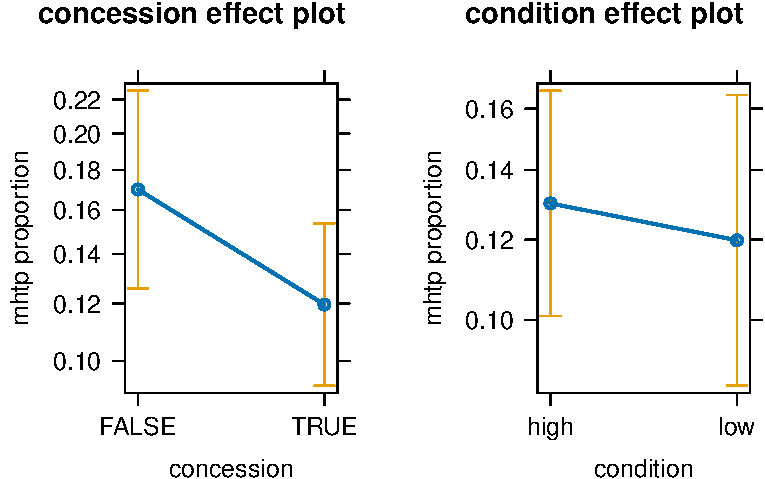
\includegraphics[keepaspectratio]{MHTP_files/figure-pdf/effects_plot_mhtp-1.pdf}}

}

\caption{\label{figure-mhtp_effects}Relationship between Mental Health
Treatment Plan (MHTP) billing and concession card status or low- vs
high- prevalence mental health condition}

\end{figure}%

\begin{figure}

\centering{

\begin{Shaded}
\begin{Highlighting}[]
\FunctionTok{plot}\NormalTok{(effects}\SpecialCharTok{::}\FunctionTok{allEffects}\NormalTok{(model\_mh2713\_effects), }\AttributeTok{ylab =} \StringTok{"mh2713 proportion"}\NormalTok{)}
\end{Highlighting}
\end{Shaded}

\pandocbounded{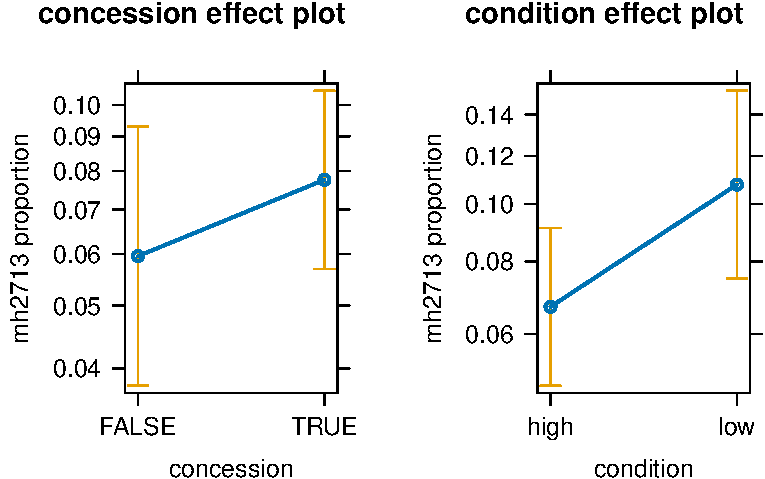
\includegraphics[keepaspectratio]{MHTP_files/figure-pdf/effects_plot_mh2713-1.pdf}}

}

\caption{\label{figure-mh2713_effects}Relationship between GP mental
health consultation (MBS item 2713) billing and concession card status
or low- vs high- prevalence mental health condition}

\end{figure}%

\begin{figure}

\centering{

\begin{Shaded}
\begin{Highlighting}[]
\FunctionTok{plot}\NormalTok{(effects}\SpecialCharTok{::}\FunctionTok{allEffects}\NormalTok{(model\_gpmp\_effects), }\AttributeTok{ylab =} \StringTok{"gpmp proportion"}\NormalTok{)}
\end{Highlighting}
\end{Shaded}

\pandocbounded{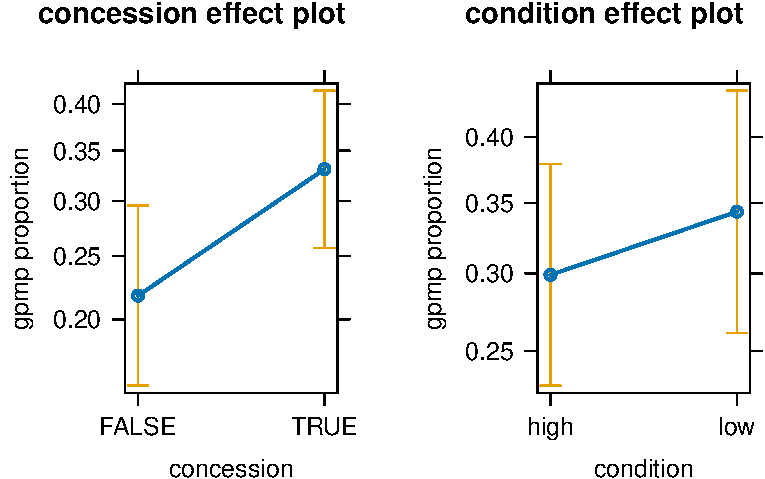
\includegraphics[keepaspectratio]{MHTP_files/figure-pdf/effects_plot_gpmp-1.pdf}}

}

\caption{\label{figure-gpmp-effects}Relationship between GP chronic
disease management plan (MBS item 721) billing and concession card
status or low- vs high- prevalence mental health condition}

\end{figure}%

\begin{table}

\centering{

\begin{Shaded}
\begin{Highlighting}[]
\NormalTok{table\_mbs\_model }\OtherTok{\textless{}{-}} \FunctionTok{modelsummary}\NormalTok{(}
  \AttributeTok{models =} \FunctionTok{list}\NormalTok{(}
    \StringTok{"MHTP"} \OtherTok{=}\NormalTok{ model\_mhtp\_effects,}
    \StringTok{"MH2713"} \OtherTok{=}\NormalTok{ model\_mh2713\_effects,}
    \StringTok{"GPMP"} \OtherTok{=}\NormalTok{ model\_gpmp\_effects}
\NormalTok{  ),}
  \AttributeTok{estimate =} \FunctionTok{c}\NormalTok{(}\StringTok{"Odds ratio"} \OtherTok{=} \StringTok{"\{estimate\}"}\NormalTok{),}
  \AttributeTok{coef\_rename =} \FunctionTok{c}\NormalTok{(}
    \StringTok{"concessionTRUE"} \OtherTok{=} \StringTok{"Concession holder"}\NormalTok{,}
    \StringTok{"conditionlow"} \OtherTok{=} \StringTok{"Low{-}prevalence condition"}
\NormalTok{  ),}
  \AttributeTok{shape =}\NormalTok{ term }\SpecialCharTok{\textasciitilde{}}\NormalTok{ model }\SpecialCharTok{+}\NormalTok{ statistic,}
  \AttributeTok{exponentiate =} \ConstantTok{TRUE}\NormalTok{,}
  \AttributeTok{statistic =} \FunctionTok{c}\NormalTok{(}\StringTok{"CI (95\%)"} \OtherTok{=} \StringTok{"[\{conf.low\}, \{conf.high\}]"}\NormalTok{, }\StringTok{"p"} \OtherTok{=} \StringTok{"\{p.value\}"}\NormalTok{),}
  \AttributeTok{output =} \StringTok{"flextable"}
\NormalTok{  ) }\SpecialCharTok{|\textgreater{}}
  \FunctionTok{my\_flextable\_theme}\NormalTok{() }\SpecialCharTok{|\textgreater{}}
  \FunctionTok{fontsize}\NormalTok{(}\AttributeTok{size =} \DecValTok{8}\NormalTok{, }\AttributeTok{part =} \StringTok{"all"}\NormalTok{) }\SpecialCharTok{|\textgreater{}}
  \FunctionTok{add\_footer\_lines}\NormalTok{(}
    \FunctionTok{paste}\NormalTok{(}
      \StringTok{"The odds ratio of having been billed a GP mental health treatment plan \textquotesingle{}MPTP\textquotesingle{}, GP mental health consultation \textquotesingle{}MH2713\textquotesingle{}"}\NormalTok{,}
      \StringTok{"or GP chronic disease management plan \textquotesingle{}GPMP\textquotesingle{},"}\NormalTok{,}
      \StringTok{"according to concession card status and low{-}vs{-}high prevalence mental health condition"}\NormalTok{,}
      \StringTok{"(coHealth GP clinics, May 2025)"}
\NormalTok{    )}
\NormalTok{  )}

\CommentTok{\# column width adjustment for Word (.docx) output}
\CommentTok{\# from https://stackoverflow.com/questions/70355001/how{-}to{-}fit{-}flextable{-}to{-}the{-}width{-}of{-}the{-}side{-}borders{-}in{-}the{-}word{-}document{-}outpu}
\NormalTok{w }\OtherTok{=} \DecValTok{6} \CommentTok{\# page width, in inches}
\NormalTok{auto\_widths }\OtherTok{\textless{}{-}} \FunctionTok{dim}\NormalTok{(table\_mbs\_model)}\SpecialCharTok{$}\NormalTok{widths}\SpecialCharTok{/}\FunctionTok{sum}\NormalTok{(}\FunctionTok{dim}\NormalTok{(table\_mbs\_model)}\SpecialCharTok{$}\NormalTok{widths)}
\NormalTok{table\_mbs\_model }\SpecialCharTok{|\textgreater{}}
  \FunctionTok{width}\NormalTok{(}\AttributeTok{width =}\NormalTok{ w }\SpecialCharTok{*}\NormalTok{ auto\_widths)}
\end{Highlighting}
\end{Shaded}

\global\setlength{\Oldarrayrulewidth}{\arrayrulewidth}

\global\setlength{\Oldtabcolsep}{\tabcolsep}

\setlength{\tabcolsep}{2pt}

\renewcommand*{\arraystretch}{1.5}



\providecommand{\ascline}[3]{\noalign{\global\arrayrulewidth #1}\arrayrulecolor[HTML]{#2}\cline{#3}}

\begin{longtable*}[c]{|p{1.09in}|p{0.55in}|p{0.55in}|p{0.55in}|p{0.55in}|p{0.55in}|p{0.55in}|p{0.55in}|p{0.55in}|p{0.55in}}





\multicolumn{1}{>{\centering}m{\dimexpr 1.09in+0\tabcolsep}}{\textcolor[HTML]{000000}{\fontsize{8}{8}\selectfont{\global\setmainfont{DejaVu Sans}{\textbf{\ }}}}} & \multicolumn{3}{>{\centering}m{\dimexpr 1.64in+4\tabcolsep}}{\textcolor[HTML]{000000}{\fontsize{8}{8}\selectfont{\global\setmainfont{DejaVu Sans}{\textbf{MHTP}}}}} & \multicolumn{3}{>{\centering}m{\dimexpr 1.64in+4\tabcolsep}}{\textcolor[HTML]{000000}{\fontsize{8}{8}\selectfont{\global\setmainfont{DejaVu Sans}{\textbf{MH2713}}}}} & \multicolumn{3}{>{\centering}m{\dimexpr 1.64in+4\tabcolsep}}{\textcolor[HTML]{000000}{\fontsize{8}{8}\selectfont{\global\setmainfont{DejaVu Sans}{\textbf{GPMP}}}}} \\

\ascline{0.5pt}{BEBEBE}{2-10}



\multicolumn{1}{>{\raggedright}m{\dimexpr 1.09in+0\tabcolsep}}{\textcolor[HTML]{000000}{\fontsize{8}{8}\selectfont{\global\setmainfont{DejaVu Sans}{\textbf{\ }}}}} & \multicolumn{1}{>{\raggedright}m{\dimexpr 0.55in+0\tabcolsep}}{\textcolor[HTML]{000000}{\fontsize{8}{8}\selectfont{\global\setmainfont{DejaVu Sans}{\textbf{Odds\ ratio}}}}} & \multicolumn{1}{>{\raggedright}m{\dimexpr 0.55in+0\tabcolsep}}{\textcolor[HTML]{000000}{\fontsize{8}{8}\selectfont{\global\setmainfont{DejaVu Sans}{\textbf{CI\ (95\%)}}}}} & \multicolumn{1}{>{\raggedright}m{\dimexpr 0.55in+0\tabcolsep}}{\textcolor[HTML]{000000}{\fontsize{8}{8}\selectfont{\global\setmainfont{DejaVu Sans}{\textbf{p}}}}} & \multicolumn{1}{>{\raggedright}m{\dimexpr 0.55in+0\tabcolsep}}{\textcolor[HTML]{000000}{\fontsize{8}{8}\selectfont{\global\setmainfont{DejaVu Sans}{\textbf{Odds\ ratio\ }}}}} & \multicolumn{1}{>{\raggedright}m{\dimexpr 0.55in+0\tabcolsep}}{\textcolor[HTML]{000000}{\fontsize{8}{8}\selectfont{\global\setmainfont{DejaVu Sans}{\textbf{CI\ (95\%)\ }}}}} & \multicolumn{1}{>{\raggedright}m{\dimexpr 0.55in+0\tabcolsep}}{\textcolor[HTML]{000000}{\fontsize{8}{8}\selectfont{\global\setmainfont{DejaVu Sans}{\textbf{p\ }}}}} & \multicolumn{1}{>{\raggedright}m{\dimexpr 0.55in+0\tabcolsep}}{\textcolor[HTML]{000000}{\fontsize{8}{8}\selectfont{\global\setmainfont{DejaVu Sans}{\textbf{Odds\ ratio\ \ }}}}} & \multicolumn{1}{>{\raggedright}m{\dimexpr 0.55in+0\tabcolsep}}{\textcolor[HTML]{000000}{\fontsize{8}{8}\selectfont{\global\setmainfont{DejaVu Sans}{\textbf{CI\ (95\%)\ \ }}}}} & \multicolumn{1}{>{\raggedright}m{\dimexpr 0.55in+0\tabcolsep}}{\textcolor[HTML]{000000}{\fontsize{8}{8}\selectfont{\global\setmainfont{DejaVu Sans}{\textbf{p\ \ }}}}} \\

\ascline{1pt}{666666}{1-10}\endfirsthead 



\multicolumn{1}{>{\centering}m{\dimexpr 1.09in+0\tabcolsep}}{\textcolor[HTML]{000000}{\fontsize{8}{8}\selectfont{\global\setmainfont{DejaVu Sans}{\textbf{\ }}}}} & \multicolumn{3}{>{\centering}m{\dimexpr 1.64in+4\tabcolsep}}{\textcolor[HTML]{000000}{\fontsize{8}{8}\selectfont{\global\setmainfont{DejaVu Sans}{\textbf{MHTP}}}}} & \multicolumn{3}{>{\centering}m{\dimexpr 1.64in+4\tabcolsep}}{\textcolor[HTML]{000000}{\fontsize{8}{8}\selectfont{\global\setmainfont{DejaVu Sans}{\textbf{MH2713}}}}} & \multicolumn{3}{>{\centering}m{\dimexpr 1.64in+4\tabcolsep}}{\textcolor[HTML]{000000}{\fontsize{8}{8}\selectfont{\global\setmainfont{DejaVu Sans}{\textbf{GPMP}}}}} \\

\ascline{0.5pt}{BEBEBE}{2-10}



\multicolumn{1}{>{\raggedright}m{\dimexpr 1.09in+0\tabcolsep}}{\textcolor[HTML]{000000}{\fontsize{8}{8}\selectfont{\global\setmainfont{DejaVu Sans}{\textbf{\ }}}}} & \multicolumn{1}{>{\raggedright}m{\dimexpr 0.55in+0\tabcolsep}}{\textcolor[HTML]{000000}{\fontsize{8}{8}\selectfont{\global\setmainfont{DejaVu Sans}{\textbf{Odds\ ratio}}}}} & \multicolumn{1}{>{\raggedright}m{\dimexpr 0.55in+0\tabcolsep}}{\textcolor[HTML]{000000}{\fontsize{8}{8}\selectfont{\global\setmainfont{DejaVu Sans}{\textbf{CI\ (95\%)}}}}} & \multicolumn{1}{>{\raggedright}m{\dimexpr 0.55in+0\tabcolsep}}{\textcolor[HTML]{000000}{\fontsize{8}{8}\selectfont{\global\setmainfont{DejaVu Sans}{\textbf{p}}}}} & \multicolumn{1}{>{\raggedright}m{\dimexpr 0.55in+0\tabcolsep}}{\textcolor[HTML]{000000}{\fontsize{8}{8}\selectfont{\global\setmainfont{DejaVu Sans}{\textbf{Odds\ ratio\ }}}}} & \multicolumn{1}{>{\raggedright}m{\dimexpr 0.55in+0\tabcolsep}}{\textcolor[HTML]{000000}{\fontsize{8}{8}\selectfont{\global\setmainfont{DejaVu Sans}{\textbf{CI\ (95\%)\ }}}}} & \multicolumn{1}{>{\raggedright}m{\dimexpr 0.55in+0\tabcolsep}}{\textcolor[HTML]{000000}{\fontsize{8}{8}\selectfont{\global\setmainfont{DejaVu Sans}{\textbf{p\ }}}}} & \multicolumn{1}{>{\raggedright}m{\dimexpr 0.55in+0\tabcolsep}}{\textcolor[HTML]{000000}{\fontsize{8}{8}\selectfont{\global\setmainfont{DejaVu Sans}{\textbf{Odds\ ratio\ \ }}}}} & \multicolumn{1}{>{\raggedright}m{\dimexpr 0.55in+0\tabcolsep}}{\textcolor[HTML]{000000}{\fontsize{8}{8}\selectfont{\global\setmainfont{DejaVu Sans}{\textbf{CI\ (95\%)\ \ }}}}} & \multicolumn{1}{>{\raggedright}m{\dimexpr 0.55in+0\tabcolsep}}{\textcolor[HTML]{000000}{\fontsize{8}{8}\selectfont{\global\setmainfont{DejaVu Sans}{\textbf{p\ \ }}}}} \\

\ascline{1pt}{666666}{1-10}\endhead



\multicolumn{1}{>{\raggedright}m{\dimexpr 1.09in+0\tabcolsep}}{\textcolor[HTML]{000000}{\fontsize{8}{8}\selectfont{\global\setmainfont{DejaVu Sans}{(Intercept)}}}} & \multicolumn{1}{>{\raggedright}m{\dimexpr 0.55in+0\tabcolsep}}{\textcolor[HTML]{000000}{\fontsize{8}{8}\selectfont{\global\setmainfont{DejaVu Sans}{0.209}}}} & \multicolumn{1}{>{\raggedright}m{\dimexpr 0.55in+0\tabcolsep}}{\textcolor[HTML]{000000}{\fontsize{8}{8}\selectfont{\global\setmainfont{DejaVu Sans}{[0.147,\ 0.297]}}}} & \multicolumn{1}{>{\raggedright}m{\dimexpr 0.55in+0\tabcolsep}}{\textcolor[HTML]{000000}{\fontsize{8}{8}\selectfont{\global\setmainfont{DejaVu Sans}{<0.001}}}} & \multicolumn{1}{>{\raggedright}m{\dimexpr 0.55in+0\tabcolsep}}{\textcolor[HTML]{000000}{\fontsize{8}{8}\selectfont{\global\setmainfont{DejaVu Sans}{0.057}}}} & \multicolumn{1}{>{\raggedright}m{\dimexpr 0.55in+0\tabcolsep}}{\textcolor[HTML]{000000}{\fontsize{8}{8}\selectfont{\global\setmainfont{DejaVu Sans}{[0.035,\ 0.092]}}}} & \multicolumn{1}{>{\raggedright}m{\dimexpr 0.55in+0\tabcolsep}}{\textcolor[HTML]{000000}{\fontsize{8}{8}\selectfont{\global\setmainfont{DejaVu Sans}{<0.001}}}} & \multicolumn{1}{>{\raggedright}m{\dimexpr 0.55in+0\tabcolsep}}{\textcolor[HTML]{000000}{\fontsize{8}{8}\selectfont{\global\setmainfont{DejaVu Sans}{0.267}}}} & \multicolumn{1}{>{\raggedright}m{\dimexpr 0.55in+0\tabcolsep}}{\textcolor[HTML]{000000}{\fontsize{8}{8}\selectfont{\global\setmainfont{DejaVu Sans}{[0.177,\ 0.402]}}}} & \multicolumn{1}{>{\raggedright}m{\dimexpr 0.55in+0\tabcolsep}}{\textcolor[HTML]{000000}{\fontsize{8}{8}\selectfont{\global\setmainfont{DejaVu Sans}{<0.001}}}} \\





\multicolumn{1}{>{\raggedright}m{\dimexpr 1.09in+0\tabcolsep}}{\textcolor[HTML]{000000}{\fontsize{8}{8}\selectfont{\global\setmainfont{DejaVu Sans}{Concession\ holder}}}} & \multicolumn{1}{>{\raggedright}m{\dimexpr 0.55in+0\tabcolsep}}{\textcolor[HTML]{000000}{\fontsize{8}{8}\selectfont{\global\setmainfont{DejaVu Sans}{0.664}}}} & \multicolumn{1}{>{\raggedright}m{\dimexpr 0.55in+0\tabcolsep}}{\textcolor[HTML]{000000}{\fontsize{8}{8}\selectfont{\global\setmainfont{DejaVu Sans}{[0.500,\ 0.880]}}}} & \multicolumn{1}{>{\raggedright}m{\dimexpr 0.55in+0\tabcolsep}}{\textcolor[HTML]{000000}{\fontsize{8}{8}\selectfont{\global\setmainfont{DejaVu Sans}{0.004}}}} & \multicolumn{1}{>{\raggedright}m{\dimexpr 0.55in+0\tabcolsep}}{\textcolor[HTML]{000000}{\fontsize{8}{8}\selectfont{\global\setmainfont{DejaVu Sans}{1.329}}}} & \multicolumn{1}{>{\raggedright}m{\dimexpr 0.55in+0\tabcolsep}}{\textcolor[HTML]{000000}{\fontsize{8}{8}\selectfont{\global\setmainfont{DejaVu Sans}{[0.866,\ 2.039]}}}} & \multicolumn{1}{>{\raggedright}m{\dimexpr 0.55in+0\tabcolsep}}{\textcolor[HTML]{000000}{\fontsize{8}{8}\selectfont{\global\setmainfont{DejaVu Sans}{0.193}}}} & \multicolumn{1}{>{\raggedright}m{\dimexpr 0.55in+0\tabcolsep}}{\textcolor[HTML]{000000}{\fontsize{8}{8}\selectfont{\global\setmainfont{DejaVu Sans}{1.779}}}} & \multicolumn{1}{>{\raggedright}m{\dimexpr 0.55in+0\tabcolsep}}{\textcolor[HTML]{000000}{\fontsize{8}{8}\selectfont{\global\setmainfont{DejaVu Sans}{[1.393,\ 2.272]}}}} & \multicolumn{1}{>{\raggedright}m{\dimexpr 0.55in+0\tabcolsep}}{\textcolor[HTML]{000000}{\fontsize{8}{8}\selectfont{\global\setmainfont{DejaVu Sans}{<0.001}}}} \\





\multicolumn{1}{>{\raggedright}m{\dimexpr 1.09in+0\tabcolsep}}{\textcolor[HTML]{000000}{\fontsize{8}{8}\selectfont{\global\setmainfont{DejaVu Sans}{Low-prevalence\ condition}}}} & \multicolumn{1}{>{\raggedright}m{\dimexpr 0.55in+0\tabcolsep}}{\textcolor[HTML]{000000}{\fontsize{8}{8}\selectfont{\global\setmainfont{DejaVu Sans}{0.910}}}} & \multicolumn{1}{>{\raggedright}m{\dimexpr 0.55in+0\tabcolsep}}{\textcolor[HTML]{000000}{\fontsize{8}{8}\selectfont{\global\setmainfont{DejaVu Sans}{[0.672,\ 1.232]}}}} & \multicolumn{1}{>{\raggedright}m{\dimexpr 0.55in+0\tabcolsep}}{\textcolor[HTML]{000000}{\fontsize{8}{8}\selectfont{\global\setmainfont{DejaVu Sans}{0.543}}}} & \multicolumn{1}{>{\raggedright}m{\dimexpr 0.55in+0\tabcolsep}}{\textcolor[HTML]{000000}{\fontsize{8}{8}\selectfont{\global\setmainfont{DejaVu Sans}{1.685}}}} & \multicolumn{1}{>{\raggedright}m{\dimexpr 0.55in+0\tabcolsep}}{\textcolor[HTML]{000000}{\fontsize{8}{8}\selectfont{\global\setmainfont{DejaVu Sans}{[1.208,\ 2.350]}}}} & \multicolumn{1}{>{\raggedright}m{\dimexpr 0.55in+0\tabcolsep}}{\textcolor[HTML]{000000}{\fontsize{8}{8}\selectfont{\global\setmainfont{DejaVu Sans}{0.002}}}} & \multicolumn{1}{>{\raggedright}m{\dimexpr 0.55in+0\tabcolsep}}{\textcolor[HTML]{000000}{\fontsize{8}{8}\selectfont{\global\setmainfont{DejaVu Sans}{1.227}}}} & \multicolumn{1}{>{\raggedright}m{\dimexpr 0.55in+0\tabcolsep}}{\textcolor[HTML]{000000}{\fontsize{8}{8}\selectfont{\global\setmainfont{DejaVu Sans}{[0.992,\ 1.516]}}}} & \multicolumn{1}{>{\raggedright}m{\dimexpr 0.55in+0\tabcolsep}}{\textcolor[HTML]{000000}{\fontsize{8}{8}\selectfont{\global\setmainfont{DejaVu Sans}{0.059}}}} \\





\multicolumn{1}{>{\raggedright}m{\dimexpr 1.09in+0\tabcolsep}}{\textcolor[HTML]{000000}{\fontsize{8}{8}\selectfont{\global\setmainfont{DejaVu Sans}{SD\ (Intercept\ clinic)}}}} & \multicolumn{1}{>{\raggedright}m{\dimexpr 0.55in+0\tabcolsep}}{\textcolor[HTML]{000000}{\fontsize{8}{8}\selectfont{\global\setmainfont{DejaVu Sans}{1.330}}}} & \multicolumn{1}{>{\raggedright}m{\dimexpr 0.55in+0\tabcolsep}}{\textcolor[HTML]{000000}{\fontsize{8}{8}\selectfont{\global\setmainfont{DejaVu Sans}{}}}} & \multicolumn{1}{>{\raggedright}m{\dimexpr 0.55in+0\tabcolsep}}{\textcolor[HTML]{000000}{\fontsize{8}{8}\selectfont{\global\setmainfont{DejaVu Sans}{}}}} & \multicolumn{1}{>{\raggedright}m{\dimexpr 0.55in+0\tabcolsep}}{\textcolor[HTML]{000000}{\fontsize{8}{8}\selectfont{\global\setmainfont{DejaVu Sans}{1.377}}}} & \multicolumn{1}{>{\raggedright}m{\dimexpr 0.55in+0\tabcolsep}}{\textcolor[HTML]{000000}{\fontsize{8}{8}\selectfont{\global\setmainfont{DejaVu Sans}{}}}} & \multicolumn{1}{>{\raggedright}m{\dimexpr 0.55in+0\tabcolsep}}{\textcolor[HTML]{000000}{\fontsize{8}{8}\selectfont{\global\setmainfont{DejaVu Sans}{}}}} & \multicolumn{1}{>{\raggedright}m{\dimexpr 0.55in+0\tabcolsep}}{\textcolor[HTML]{000000}{\fontsize{8}{8}\selectfont{\global\setmainfont{DejaVu Sans}{1.478}}}} & \multicolumn{1}{>{\raggedright}m{\dimexpr 0.55in+0\tabcolsep}}{\textcolor[HTML]{000000}{\fontsize{8}{8}\selectfont{\global\setmainfont{DejaVu Sans}{}}}} & \multicolumn{1}{>{\raggedright}m{\dimexpr 0.55in+0\tabcolsep}}{\textcolor[HTML]{000000}{\fontsize{8}{8}\selectfont{\global\setmainfont{DejaVu Sans}{}}}} \\

\ascline{0.5pt}{BEBEBE}{1-10}



\multicolumn{1}{>{\raggedright}m{\dimexpr 1.09in+0\tabcolsep}}{\textcolor[HTML]{000000}{\fontsize{8}{8}\selectfont{\global\setmainfont{DejaVu Sans}{Num.Obs.}}}} & \multicolumn{1}{>{\raggedright}m{\dimexpr 0.55in+0\tabcolsep}}{\textcolor[HTML]{000000}{\fontsize{8}{8}\selectfont{\global\setmainfont{DejaVu Sans}{2544}}}} & \multicolumn{1}{>{\raggedright}m{\dimexpr 0.55in+0\tabcolsep}}{\textcolor[HTML]{000000}{\fontsize{8}{8}\selectfont{\global\setmainfont{DejaVu Sans}{}}}} & \multicolumn{1}{>{\raggedright}m{\dimexpr 0.55in+0\tabcolsep}}{\textcolor[HTML]{000000}{\fontsize{8}{8}\selectfont{\global\setmainfont{DejaVu Sans}{}}}} & \multicolumn{1}{>{\raggedright}m{\dimexpr 0.55in+0\tabcolsep}}{\textcolor[HTML]{000000}{\fontsize{8}{8}\selectfont{\global\setmainfont{DejaVu Sans}{2544}}}} & \multicolumn{1}{>{\raggedright}m{\dimexpr 0.55in+0\tabcolsep}}{\textcolor[HTML]{000000}{\fontsize{8}{8}\selectfont{\global\setmainfont{DejaVu Sans}{}}}} & \multicolumn{1}{>{\raggedright}m{\dimexpr 0.55in+0\tabcolsep}}{\textcolor[HTML]{000000}{\fontsize{8}{8}\selectfont{\global\setmainfont{DejaVu Sans}{}}}} & \multicolumn{1}{>{\raggedright}m{\dimexpr 0.55in+0\tabcolsep}}{\textcolor[HTML]{000000}{\fontsize{8}{8}\selectfont{\global\setmainfont{DejaVu Sans}{2544}}}} & \multicolumn{1}{>{\raggedright}m{\dimexpr 0.55in+0\tabcolsep}}{\textcolor[HTML]{000000}{\fontsize{8}{8}\selectfont{\global\setmainfont{DejaVu Sans}{}}}} & \multicolumn{1}{>{\raggedright}m{\dimexpr 0.55in+0\tabcolsep}}{\textcolor[HTML]{000000}{\fontsize{8}{8}\selectfont{\global\setmainfont{DejaVu Sans}{}}}} \\





\multicolumn{1}{>{\raggedright}m{\dimexpr 1.09in+0\tabcolsep}}{\textcolor[HTML]{000000}{\fontsize{8}{8}\selectfont{\global\setmainfont{DejaVu Sans}{R2\ Marg.}}}} & \multicolumn{1}{>{\raggedright}m{\dimexpr 0.55in+0\tabcolsep}}{\textcolor[HTML]{000000}{\fontsize{8}{8}\selectfont{\global\setmainfont{DejaVu Sans}{0.008}}}} & \multicolumn{1}{>{\raggedright}m{\dimexpr 0.55in+0\tabcolsep}}{\textcolor[HTML]{000000}{\fontsize{8}{8}\selectfont{\global\setmainfont{DejaVu Sans}{}}}} & \multicolumn{1}{>{\raggedright}m{\dimexpr 0.55in+0\tabcolsep}}{\textcolor[HTML]{000000}{\fontsize{8}{8}\selectfont{\global\setmainfont{DejaVu Sans}{}}}} & \multicolumn{1}{>{\raggedright}m{\dimexpr 0.55in+0\tabcolsep}}{\textcolor[HTML]{000000}{\fontsize{8}{8}\selectfont{\global\setmainfont{DejaVu Sans}{0.018}}}} & \multicolumn{1}{>{\raggedright}m{\dimexpr 0.55in+0\tabcolsep}}{\textcolor[HTML]{000000}{\fontsize{8}{8}\selectfont{\global\setmainfont{DejaVu Sans}{}}}} & \multicolumn{1}{>{\raggedright}m{\dimexpr 0.55in+0\tabcolsep}}{\textcolor[HTML]{000000}{\fontsize{8}{8}\selectfont{\global\setmainfont{DejaVu Sans}{}}}} & \multicolumn{1}{>{\raggedright}m{\dimexpr 0.55in+0\tabcolsep}}{\textcolor[HTML]{000000}{\fontsize{8}{8}\selectfont{\global\setmainfont{DejaVu Sans}{0.018}}}} & \multicolumn{1}{>{\raggedright}m{\dimexpr 0.55in+0\tabcolsep}}{\textcolor[HTML]{000000}{\fontsize{8}{8}\selectfont{\global\setmainfont{DejaVu Sans}{}}}} & \multicolumn{1}{>{\raggedright}m{\dimexpr 0.55in+0\tabcolsep}}{\textcolor[HTML]{000000}{\fontsize{8}{8}\selectfont{\global\setmainfont{DejaVu Sans}{}}}} \\





\multicolumn{1}{>{\raggedright}m{\dimexpr 1.09in+0\tabcolsep}}{\textcolor[HTML]{000000}{\fontsize{8}{8}\selectfont{\global\setmainfont{DejaVu Sans}{R2\ Cond.}}}} & \multicolumn{1}{>{\raggedright}m{\dimexpr 0.55in+0\tabcolsep}}{\textcolor[HTML]{000000}{\fontsize{8}{8}\selectfont{\global\setmainfont{DejaVu Sans}{0.032}}}} & \multicolumn{1}{>{\raggedright}m{\dimexpr 0.55in+0\tabcolsep}}{\textcolor[HTML]{000000}{\fontsize{8}{8}\selectfont{\global\setmainfont{DejaVu Sans}{}}}} & \multicolumn{1}{>{\raggedright}m{\dimexpr 0.55in+0\tabcolsep}}{\textcolor[HTML]{000000}{\fontsize{8}{8}\selectfont{\global\setmainfont{DejaVu Sans}{}}}} & \multicolumn{1}{>{\raggedright}m{\dimexpr 0.55in+0\tabcolsep}}{\textcolor[HTML]{000000}{\fontsize{8}{8}\selectfont{\global\setmainfont{DejaVu Sans}{0.048}}}} & \multicolumn{1}{>{\raggedright}m{\dimexpr 0.55in+0\tabcolsep}}{\textcolor[HTML]{000000}{\fontsize{8}{8}\selectfont{\global\setmainfont{DejaVu Sans}{}}}} & \multicolumn{1}{>{\raggedright}m{\dimexpr 0.55in+0\tabcolsep}}{\textcolor[HTML]{000000}{\fontsize{8}{8}\selectfont{\global\setmainfont{DejaVu Sans}{}}}} & \multicolumn{1}{>{\raggedright}m{\dimexpr 0.55in+0\tabcolsep}}{\textcolor[HTML]{000000}{\fontsize{8}{8}\selectfont{\global\setmainfont{DejaVu Sans}{0.061}}}} & \multicolumn{1}{>{\raggedright}m{\dimexpr 0.55in+0\tabcolsep}}{\textcolor[HTML]{000000}{\fontsize{8}{8}\selectfont{\global\setmainfont{DejaVu Sans}{}}}} & \multicolumn{1}{>{\raggedright}m{\dimexpr 0.55in+0\tabcolsep}}{\textcolor[HTML]{000000}{\fontsize{8}{8}\selectfont{\global\setmainfont{DejaVu Sans}{}}}} \\





\multicolumn{1}{>{\raggedright}m{\dimexpr 1.09in+0\tabcolsep}}{\textcolor[HTML]{000000}{\fontsize{8}{8}\selectfont{\global\setmainfont{DejaVu Sans}{AIC}}}} & \multicolumn{1}{>{\raggedright}m{\dimexpr 0.55in+0\tabcolsep}}{\textcolor[HTML]{000000}{\fontsize{8}{8}\selectfont{\global\setmainfont{DejaVu Sans}{1922.6}}}} & \multicolumn{1}{>{\raggedright}m{\dimexpr 0.55in+0\tabcolsep}}{\textcolor[HTML]{000000}{\fontsize{8}{8}\selectfont{\global\setmainfont{DejaVu Sans}{}}}} & \multicolumn{1}{>{\raggedright}m{\dimexpr 0.55in+0\tabcolsep}}{\textcolor[HTML]{000000}{\fontsize{8}{8}\selectfont{\global\setmainfont{DejaVu Sans}{}}}} & \multicolumn{1}{>{\raggedright}m{\dimexpr 0.55in+0\tabcolsep}}{\textcolor[HTML]{000000}{\fontsize{8}{8}\selectfont{\global\setmainfont{DejaVu Sans}{1335.8}}}} & \multicolumn{1}{>{\raggedright}m{\dimexpr 0.55in+0\tabcolsep}}{\textcolor[HTML]{000000}{\fontsize{8}{8}\selectfont{\global\setmainfont{DejaVu Sans}{}}}} & \multicolumn{1}{>{\raggedright}m{\dimexpr 0.55in+0\tabcolsep}}{\textcolor[HTML]{000000}{\fontsize{8}{8}\selectfont{\global\setmainfont{DejaVu Sans}{}}}} & \multicolumn{1}{>{\raggedright}m{\dimexpr 0.55in+0\tabcolsep}}{\textcolor[HTML]{000000}{\fontsize{8}{8}\selectfont{\global\setmainfont{DejaVu Sans}{3020.7}}}} & \multicolumn{1}{>{\raggedright}m{\dimexpr 0.55in+0\tabcolsep}}{\textcolor[HTML]{000000}{\fontsize{8}{8}\selectfont{\global\setmainfont{DejaVu Sans}{}}}} & \multicolumn{1}{>{\raggedright}m{\dimexpr 0.55in+0\tabcolsep}}{\textcolor[HTML]{000000}{\fontsize{8}{8}\selectfont{\global\setmainfont{DejaVu Sans}{}}}} \\





\multicolumn{1}{>{\raggedright}m{\dimexpr 1.09in+0\tabcolsep}}{\textcolor[HTML]{000000}{\fontsize{8}{8}\selectfont{\global\setmainfont{DejaVu Sans}{BIC}}}} & \multicolumn{1}{>{\raggedright}m{\dimexpr 0.55in+0\tabcolsep}}{\textcolor[HTML]{000000}{\fontsize{8}{8}\selectfont{\global\setmainfont{DejaVu Sans}{1946.0}}}} & \multicolumn{1}{>{\raggedright}m{\dimexpr 0.55in+0\tabcolsep}}{\textcolor[HTML]{000000}{\fontsize{8}{8}\selectfont{\global\setmainfont{DejaVu Sans}{}}}} & \multicolumn{1}{>{\raggedright}m{\dimexpr 0.55in+0\tabcolsep}}{\textcolor[HTML]{000000}{\fontsize{8}{8}\selectfont{\global\setmainfont{DejaVu Sans}{}}}} & \multicolumn{1}{>{\raggedright}m{\dimexpr 0.55in+0\tabcolsep}}{\textcolor[HTML]{000000}{\fontsize{8}{8}\selectfont{\global\setmainfont{DejaVu Sans}{1359.1}}}} & \multicolumn{1}{>{\raggedright}m{\dimexpr 0.55in+0\tabcolsep}}{\textcolor[HTML]{000000}{\fontsize{8}{8}\selectfont{\global\setmainfont{DejaVu Sans}{}}}} & \multicolumn{1}{>{\raggedright}m{\dimexpr 0.55in+0\tabcolsep}}{\textcolor[HTML]{000000}{\fontsize{8}{8}\selectfont{\global\setmainfont{DejaVu Sans}{}}}} & \multicolumn{1}{>{\raggedright}m{\dimexpr 0.55in+0\tabcolsep}}{\textcolor[HTML]{000000}{\fontsize{8}{8}\selectfont{\global\setmainfont{DejaVu Sans}{3044.0}}}} & \multicolumn{1}{>{\raggedright}m{\dimexpr 0.55in+0\tabcolsep}}{\textcolor[HTML]{000000}{\fontsize{8}{8}\selectfont{\global\setmainfont{DejaVu Sans}{}}}} & \multicolumn{1}{>{\raggedright}m{\dimexpr 0.55in+0\tabcolsep}}{\textcolor[HTML]{000000}{\fontsize{8}{8}\selectfont{\global\setmainfont{DejaVu Sans}{}}}} \\





\multicolumn{1}{>{\raggedright}m{\dimexpr 1.09in+0\tabcolsep}}{\textcolor[HTML]{000000}{\fontsize{8}{8}\selectfont{\global\setmainfont{DejaVu Sans}{ICC}}}} & \multicolumn{1}{>{\raggedright}m{\dimexpr 0.55in+0\tabcolsep}}{\textcolor[HTML]{000000}{\fontsize{8}{8}\selectfont{\global\setmainfont{DejaVu Sans}{0.0}}}} & \multicolumn{1}{>{\raggedright}m{\dimexpr 0.55in+0\tabcolsep}}{\textcolor[HTML]{000000}{\fontsize{8}{8}\selectfont{\global\setmainfont{DejaVu Sans}{}}}} & \multicolumn{1}{>{\raggedright}m{\dimexpr 0.55in+0\tabcolsep}}{\textcolor[HTML]{000000}{\fontsize{8}{8}\selectfont{\global\setmainfont{DejaVu Sans}{}}}} & \multicolumn{1}{>{\raggedright}m{\dimexpr 0.55in+0\tabcolsep}}{\textcolor[HTML]{000000}{\fontsize{8}{8}\selectfont{\global\setmainfont{DejaVu Sans}{0.0}}}} & \multicolumn{1}{>{\raggedright}m{\dimexpr 0.55in+0\tabcolsep}}{\textcolor[HTML]{000000}{\fontsize{8}{8}\selectfont{\global\setmainfont{DejaVu Sans}{}}}} & \multicolumn{1}{>{\raggedright}m{\dimexpr 0.55in+0\tabcolsep}}{\textcolor[HTML]{000000}{\fontsize{8}{8}\selectfont{\global\setmainfont{DejaVu Sans}{}}}} & \multicolumn{1}{>{\raggedright}m{\dimexpr 0.55in+0\tabcolsep}}{\textcolor[HTML]{000000}{\fontsize{8}{8}\selectfont{\global\setmainfont{DejaVu Sans}{0.0}}}} & \multicolumn{1}{>{\raggedright}m{\dimexpr 0.55in+0\tabcolsep}}{\textcolor[HTML]{000000}{\fontsize{8}{8}\selectfont{\global\setmainfont{DejaVu Sans}{}}}} & \multicolumn{1}{>{\raggedright}m{\dimexpr 0.55in+0\tabcolsep}}{\textcolor[HTML]{000000}{\fontsize{8}{8}\selectfont{\global\setmainfont{DejaVu Sans}{}}}} \\





\multicolumn{1}{>{\raggedright}m{\dimexpr 1.09in+0\tabcolsep}}{\textcolor[HTML]{000000}{\fontsize{8}{8}\selectfont{\global\setmainfont{DejaVu Sans}{RMSE}}}} & \multicolumn{1}{>{\raggedright}m{\dimexpr 0.55in+0\tabcolsep}}{\textcolor[HTML]{000000}{\fontsize{8}{8}\selectfont{\global\setmainfont{DejaVu Sans}{0.33}}}} & \multicolumn{1}{>{\raggedright}m{\dimexpr 0.55in+0\tabcolsep}}{\textcolor[HTML]{000000}{\fontsize{8}{8}\selectfont{\global\setmainfont{DejaVu Sans}{}}}} & \multicolumn{1}{>{\raggedright}m{\dimexpr 0.55in+0\tabcolsep}}{\textcolor[HTML]{000000}{\fontsize{8}{8}\selectfont{\global\setmainfont{DejaVu Sans}{}}}} & \multicolumn{1}{>{\raggedright}m{\dimexpr 0.55in+0\tabcolsep}}{\textcolor[HTML]{000000}{\fontsize{8}{8}\selectfont{\global\setmainfont{DejaVu Sans}{0.26}}}} & \multicolumn{1}{>{\raggedright}m{\dimexpr 0.55in+0\tabcolsep}}{\textcolor[HTML]{000000}{\fontsize{8}{8}\selectfont{\global\setmainfont{DejaVu Sans}{}}}} & \multicolumn{1}{>{\raggedright}m{\dimexpr 0.55in+0\tabcolsep}}{\textcolor[HTML]{000000}{\fontsize{8}{8}\selectfont{\global\setmainfont{DejaVu Sans}{}}}} & \multicolumn{1}{>{\raggedright}m{\dimexpr 0.55in+0\tabcolsep}}{\textcolor[HTML]{000000}{\fontsize{8}{8}\selectfont{\global\setmainfont{DejaVu Sans}{0.45}}}} & \multicolumn{1}{>{\raggedright}m{\dimexpr 0.55in+0\tabcolsep}}{\textcolor[HTML]{000000}{\fontsize{8}{8}\selectfont{\global\setmainfont{DejaVu Sans}{}}}} & \multicolumn{1}{>{\raggedright}m{\dimexpr 0.55in+0\tabcolsep}}{\textcolor[HTML]{000000}{\fontsize{8}{8}\selectfont{\global\setmainfont{DejaVu Sans}{}}}} \\

\ascline{1pt}{666666}{1-10}



\multicolumn{10}{>{\raggedright}m{\dimexpr 6in+18\tabcolsep}}{\textcolor[HTML]{000000}{\fontsize{11}{11}\selectfont{\global\setmainfont{DejaVu Sans}{The\ odds\ ratio\ of\ having\ been\ billed\ a\ GP\ mental\ health\ treatment\ plan\ 'MPTP',\ GP\ mental\ health\ consultation\ 'MH2713'\ or\ GP\ chronic\ disease\ management\ plan\ 'GPMP',\ according\ to\ concession\ card\ status\ and\ low-vs-high\ prevalence\ mental\ health\ condition\ (coHealth\ GP\ clinics,\ May\ 2025)}}}} \\





\end{longtable*}



\arrayrulecolor[HTML]{000000}

\global\setlength{\arrayrulewidth}{\Oldarrayrulewidth}

\global\setlength{\tabcolsep}{\Oldtabcolsep}

\renewcommand*{\arraystretch}{1}

}

\caption{\label{table-logistic}Logistic model, MBS items by concession
status and mental health condition}

\end{table}%

\begin{figure}

\centering{

\begin{Shaded}
\begin{Highlighting}[]
\NormalTok{model\_list }\OtherTok{\textless{}{-}} \FunctionTok{list}\NormalTok{(}
  \StringTok{"MHTP"} \OtherTok{=}\NormalTok{ model\_mhtp\_effects,}
  \StringTok{"MH2713"} \OtherTok{=}\NormalTok{ model\_mh2713\_effects,}
  \StringTok{"GPMP"} \OtherTok{=}\NormalTok{ model\_gpmp\_effects}
\NormalTok{)}

\FunctionTok{modelplot}\NormalTok{(}
  \AttributeTok{models =}\NormalTok{ model\_list,}
  \AttributeTok{coef\_map =} \FunctionTok{c}\NormalTok{(}
    \StringTok{\textquotesingle{}conditionlow\textquotesingle{}} \OtherTok{=} \StringTok{"Low{-}prevalence condition"}\NormalTok{,}
    \StringTok{\textquotesingle{}concessionTRUE\textquotesingle{}} \OtherTok{=} \StringTok{"Concession holder"}
\NormalTok{  ),}
  \AttributeTok{exponentiate =} \ConstantTok{TRUE}
\NormalTok{) }\SpecialCharTok{+}
  \FunctionTok{labs}\NormalTok{(}
    \AttributeTok{x =} \StringTok{"Odds ratio estimates and 95\% confidence intervals"}\NormalTok{,}
    \AttributeTok{y =} \StringTok{"Predictors"}\NormalTok{,}
    \AttributeTok{caption =} \StringTok{"(coHealth GP clinics, May 2025)"}
\NormalTok{  ) }\SpecialCharTok{+}
  \FunctionTok{scale\_color\_manual}\NormalTok{(}\AttributeTok{values =} \FunctionTok{wes\_palette}\NormalTok{(}\StringTok{\textquotesingle{}Darjeeling1\textquotesingle{}}\NormalTok{))}
\end{Highlighting}
\end{Shaded}

\pandocbounded{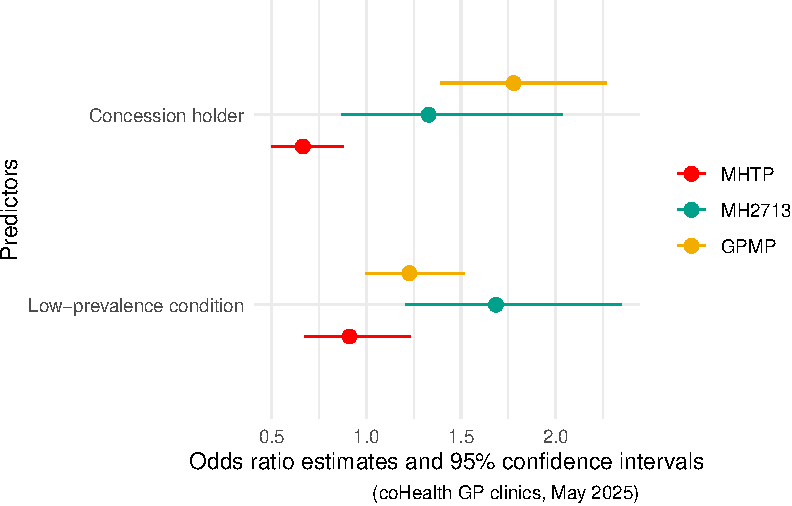
\includegraphics[keepaspectratio]{MHTP_files/figure-pdf/unnamed-chunk-8-1.pdf}}

}

\caption{\label{figure-oddsratio}MHTP, MH2713 and GPMP billed in
previous twelve months compared to concession and low- vs high-
prevalence mental health condition status. Odds ratio estimates.}

\end{figure}%

\subsection{Discussion}\label{discussion}

A relatively high proportion of coHealth patients have high-prevalence
and low-prevalence mental health conditions, but relatively few patients
at coHealth with mental health conditions have had a recent billed
mental health care plan (MHTP). Significantly fewer patients living with
a mental health condition and who have a health concession card have had
a MHTP compared to patients living with a mental health condition and
who do not have a concession card. This suggests that socio-economic
factors have a role in determining MHTP creation and billing. Patients
with low-prevalence conditions are no more likely to have an MHTP than
patients with high-prevalence conditions, although it is expected that
low-prevalence conditions are often more severe and lifelong.

Low MHTP billing may reflect low patient demand or need or awareness of
mental health treatment plans and/or access to private psychology
services. However, patients with mental health conditions and concession
cards were no less likely to have mental health consultations with the
general practitioner or chronic disease management plans compared to
patients without concession cards. Likewise, patients with
low-prevalence mental health disorders were no less likely to have
mental health consultations with the general practitioner or chronic
disease management plans than patients with high-prevalence disorders.
This suggests that identified needs exist and are catered for patients
with concession cards or low-prevalence conditions, just not with an
MHTP.

Barriers to doing an using an MHTP for patients with concession cards or
low-prevalence mental health conditions may be due to the cost of
accessing psychological services through an MHTP and the burden of
creating an MHTP.

Low access to psychology services via MHTP may be related to patients
having relatively few resources (`inverse care law'\sidenote{\footnotesize ``\href{https://doi.org/10.1016/S0140-6736(71)92410-X}{The
  Inverse Care Law}'', Julian Tudor Hart. The Lancet, Vol 297:7696 pp
  405-412, 27 February 1971.}) e.g.~pensioners and health care card
holders. Barriers to access for those with the least resources but
greater needs applies not only to mental health services, but also to
other Medicare-funded allied health services\sidenote{\footnotesize ``\href{https://grattan.edu.au/wp-content/uploads/2022/12/A-new-Medicare-strengthening-general-practice-Grattan-Report.pdf}{A
  new Medicare: Strengthening general practice}'' Breadon, P., Romanes,
  D., Fox, L., Bolton, J., and Richardson, L. Grattan Institute, 2022}.

\begin{figure}

\centering{

\pandocbounded{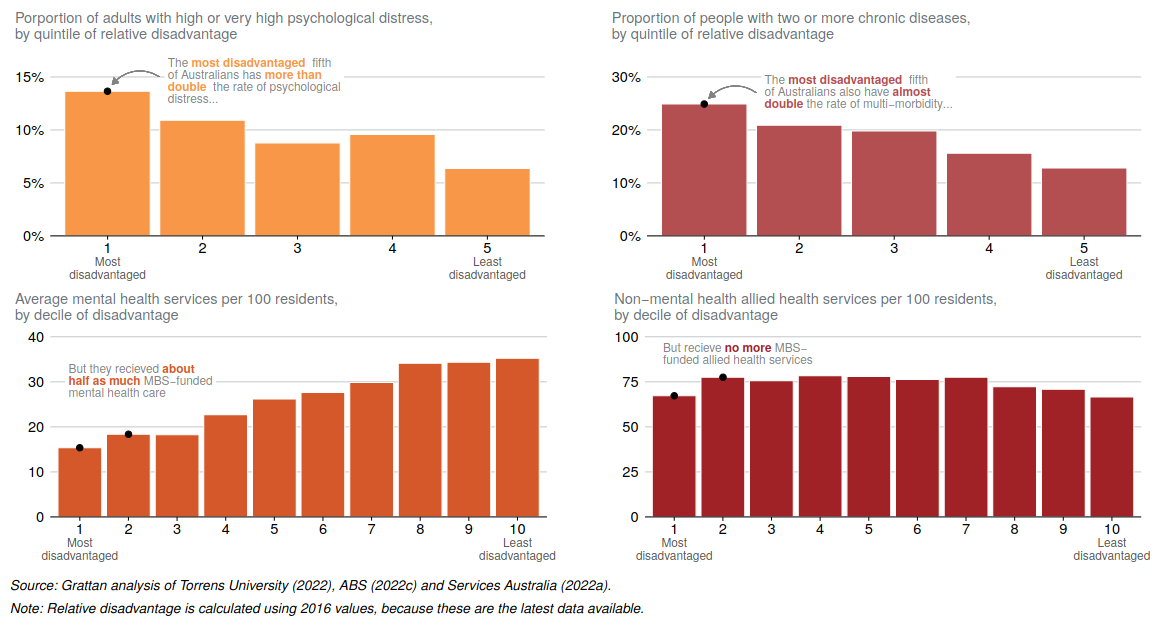
\includegraphics[keepaspectratio]{./images/Medicare_funded_alliedhealth.png}}

}

\caption{\label{figure-medicare_alliedhealth}Medicare-funded allied
health services are needed most, but used least, by more disadvantaged
Australians. `A new Medicare: Strengthening general
practice'\sidenote{\footnotesize ``\href{https://grattan.edu.au/wp-content/uploads/2022/12/A-new-Medicare-strengthening-general-practice-Grattan-Report.pdf}{A
  new Medicare: Strengthening general practice}'' Breadon, P., Romanes,
  D., Fox, L., Bolton, J., and Richardson, L. Grattan Institute, 2022},
Grattan Institute, 2022.}

\end{figure}%

If mental health care plans offer an opportunity to plan for and review
mental health care, including for patients with reduced resources,
deliberate actions may need to be considered to improve uptake of mental
health care plans among patients who already have reduced access to
healthcare.

General practitioners at cohealth have suggested:

\begin{itemize}
\item
  It could be possible to document a mental health treatment plan (MHTP)
  that is worthwhile for the patient and meet the criteria for a mental
  health treatment plan. If this could be done, then an MHTP could be
  prepared for many more patients, regardless of need for rebated
  private psychology.
\item
  Mental health treatment plan (MHTP) preparation can be done over
  several consults. Maybe preparation and `co-billing' a mental health
  care plan could be done after taking care to appropriately document
  the time and plan. Nevertheless, the effort required would still be
  considerably more than, for example, general practitioner chronic
  disease management plans. There may be a role for large-language-model
  (LLM `AI') assisted plan generation to help reduce the manual workload
  of MHTP creation.
\item
  Currently, clinic mental health nurses can help prepare mental health
  treatment plans. However, due to funding arrangements, clinic mental
  health nurse involvement is often limited to patients who are
  \emph{already} referred (or at least, will be referred) to the clinic
  mental health nurse program.
\end{itemize}

\subsection{Appendices}\label{appendices}

\subsubsection{Proportion of patients eligible and who have a mental
health treatment plan}\label{sec-appendix-mhtpeligible}

Figures derived from
\href{https://www.doctorscontrolpanel.com.au/}{Doctor's Control Panel}
`Performance' charts, for the four weeks starting from 28th April 2025.
The charts are included below.

The total number of unique patients seen during that time period can be
calculated from the numbers who are expected to have `Allergies
Documented', which is all patients seen. For cohealth, the figure is
5557+720 = 6277. For all practices which use Doctor's Control Panel
(`national'), the figure is 245991+12826 = 258817.

The total number of unique patients seen during that time period
considered eligible for a mental health treatment plan (because they
have a recorded and coded mental health condition) can be calculated
from the `MHTP' (Mental Health Treatment Plan) bar. For cohealth, the
figure is 43+441+1201+1441 = 3126, which is 49.8\% of the total. For
`national' practices, the figure is 2455+16839+34885+36287 = 90466,
which is 35.0\% of the total.

The total number of unique patients seen during that time period who had
an `up-to-date' (i.e.~within the previous twelve months) mental health
treatment plan can be calculated from the `up-to-date' and `updated'
sections of the MHTP bar. For cohealth, the figure is 43+441 = 484,
which is 15.5\% of patients with recorded mental health conditions. For
`national' practices, the figure is 2455 + 16839 = 19294, which is
21.3\% of patients with mental health conditions.

\begin{figure}

\centering{

\pandocbounded{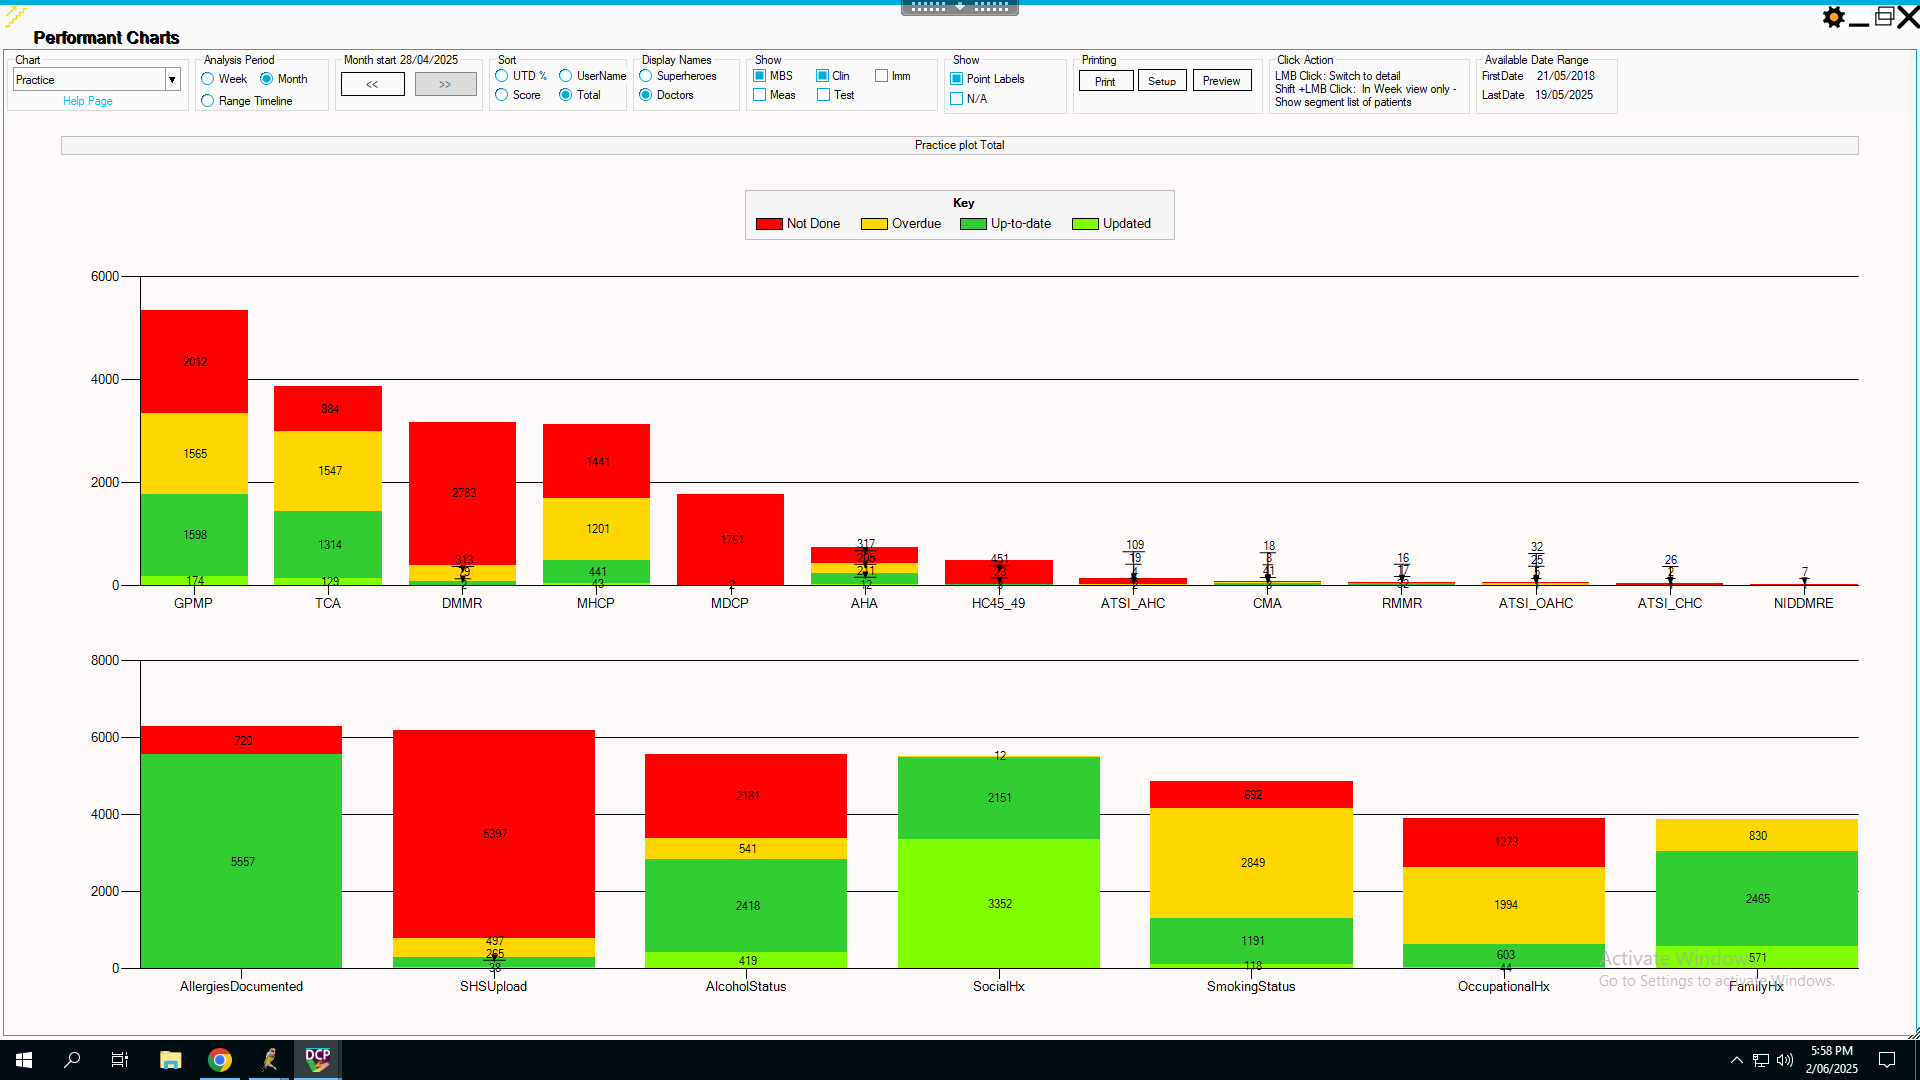
\includegraphics[keepaspectratio]{./images/cohealth_20250428_mhtpeligible.png}}

}

\caption{\label{figure-dcp_mhtpeligible}cohealth, DCP statistics,
28/Apr/2025 to 25/May/2025}

\end{figure}%

\begin{figure}

\centering{

\pandocbounded{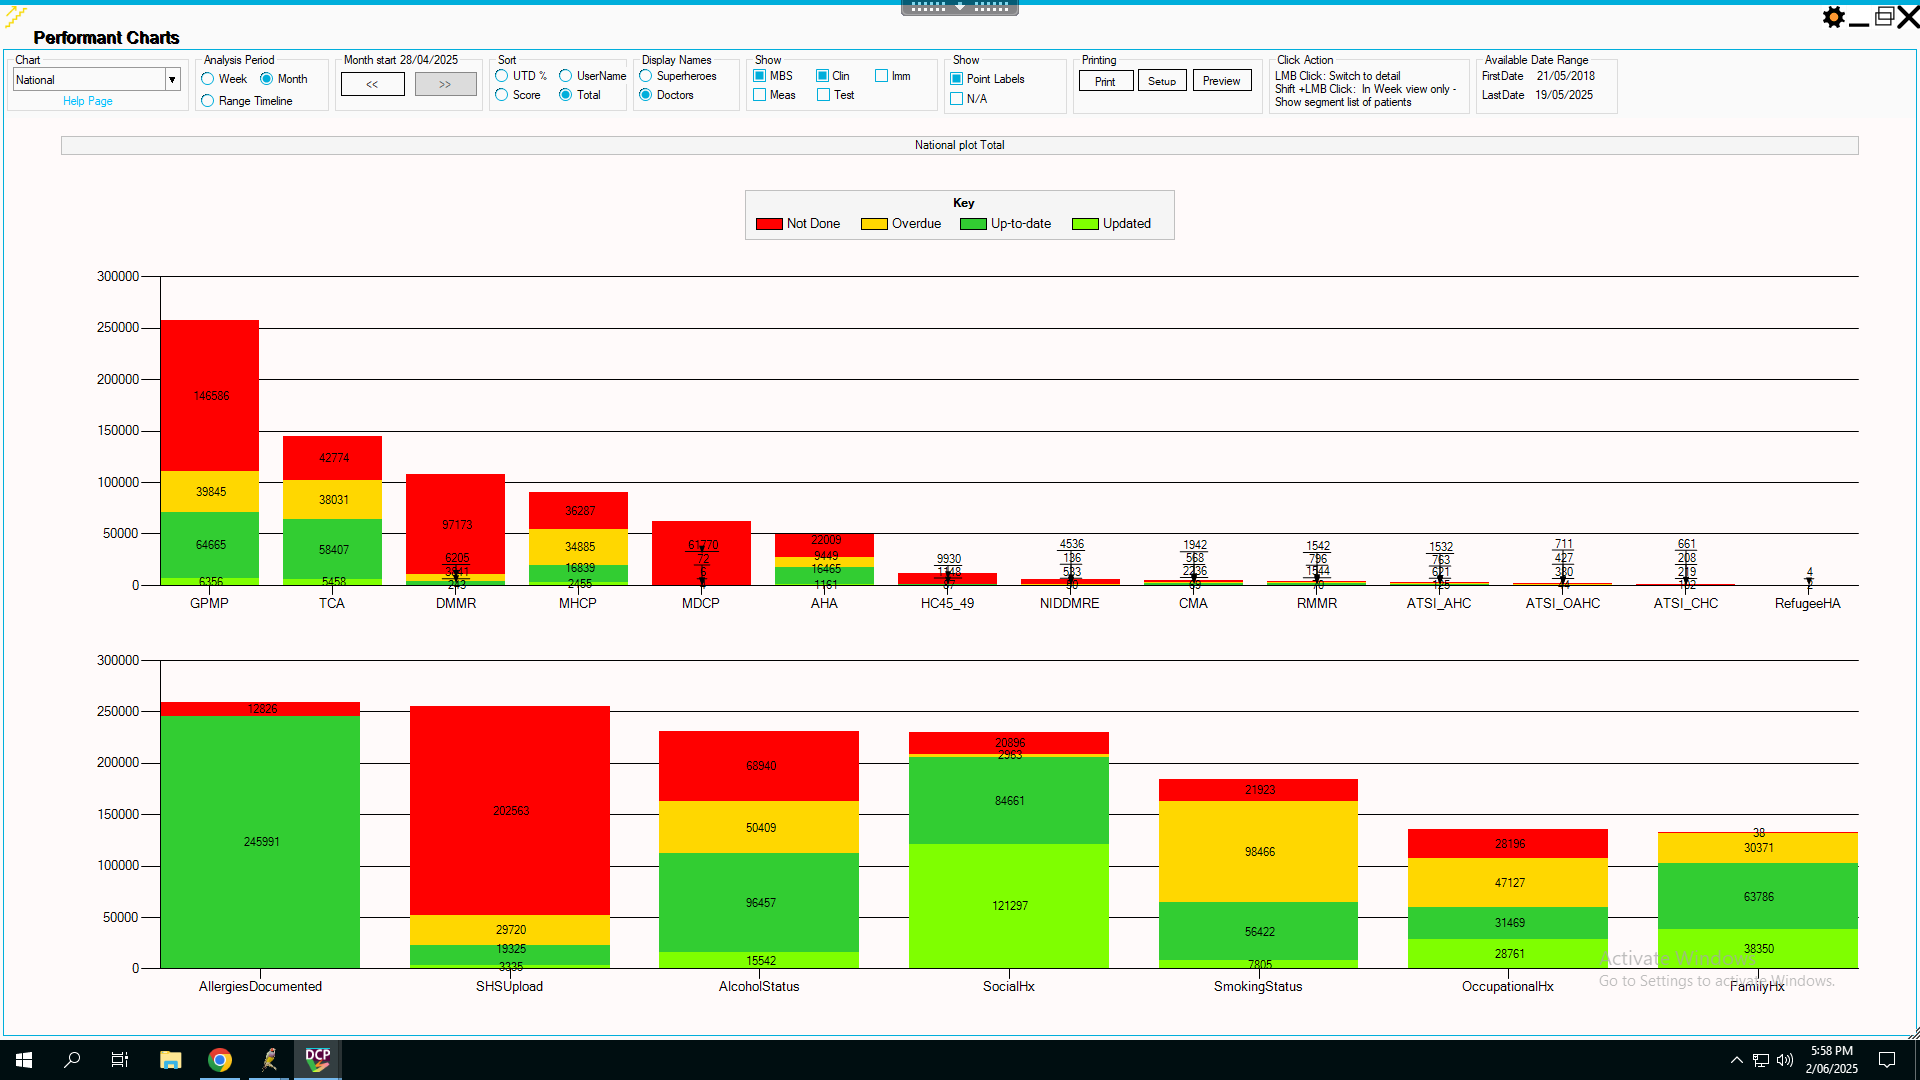
\includegraphics[keepaspectratio]{./images/national_20250428_mhtpeligible.png}}

}

\caption{\label{figure-dcp_national}National, DCP statistics,
28/Apr/2025 to 25/May/2025}

\end{figure}%

\subsubsection{Patients eligible and who have a mental health treatment
plan according to concession card status, mental health condition and
clinic attended}\label{sec-appendix-mhtpgroups}

\href{https://www.pencs.com.au/}{PenCS} was used to identify patients
with recorded mental health conditions, whether the condition was high-
or low- prevalence, concession card status, patient `activity', MBS item
numbers billed (mental health care plans, other mental health items or
chronic disease management plans) and site of attendance. The Electronic
Health Record (EHR) used was
\href{https://bestpracticesoftware.com/}{Best Practice}, the data
extract was done on 1st May 2025, a separate extract for each of five
clinic sites (Kensington, Paisley Street, Laverton, Fitzroy and
Collingwood). The period of interest is the one year from 1st May 2024
to 30th April 2025.

Patient activity:

\begin{itemize}
\tightlist
\item
  Using Filter `General'

  \begin{itemize}
  \tightlist
  \item
    Set `Start age' to `18 years' - only interested in adults
  \item
    Set `Activity' to `Active (3x in 2 yrs)' - the
    \href{https://www.racgp.org.au/running-a-practice/practice-standards/standards-5th-edition/standards-for-general-practices-5th-ed/glossary}{standard
    RACGP definition for `active patient'} is ``A patient who has
    attended the practice/service three or more times in the past two
    years''.

    \begin{itemize}
    \tightlist
    \item
      Unfortunately, PenCS has a longstanding problem of often counting
      `activity' as including items such as recording third-party
      telephone calls, writing letters without seeing the patient etc..
      Some patients identified as `active' using that criteria were
      never consulted at all during the two year period! For this
      reason, an additional filter is added based on Medicare Benefit
      Schedule (MBS) billing.
    \end{itemize}
  \end{itemize}
\item
  Using Filter `MBS Attendance'

  \begin{itemize}
  \tightlist
  \item
    Filtering to patients who have had an MBS billing helps reduce the
    number of patients identified as `active' who had no meaningful
    contact (a billable consult) with the clinic.

    \begin{itemize}
    \tightlist
    \item
      There are \emph{some} patients who are seen without being billed
      e.g.~asylum seekers. However, in that case, those patients would
      also not be eligible to be billed mental health care plans, mental
      health consult items, care plans etc..
    \end{itemize}
  \item
    Set location to ``My Locations Only'' - This restrict the MBS filter
    to billing done at the site of interest.
  \item
    Set `Claim Date Range' to `\textless= 12 months'
  \item
    Set `MBS Item Numbers' to `Any of selected', and choose item numbers
    ``3, 23, 36, 44, 123, 2713, 91890, 91891, 721, 723, 732, 701, 703,
    705, 707, 2700, 2701, 2712, 2715, 2717''. These item number include
    most of the common item numbers.

    \begin{itemize}
    \tightlist
    \item
      Choosing the most common item numbers was not actually necessary.
      By not selecting any item numbers in this panel, the default
      search appears to be `any item number'.
    \end{itemize}
  \end{itemize}
\end{itemize}

\begin{figure}

\centering{

\pandocbounded{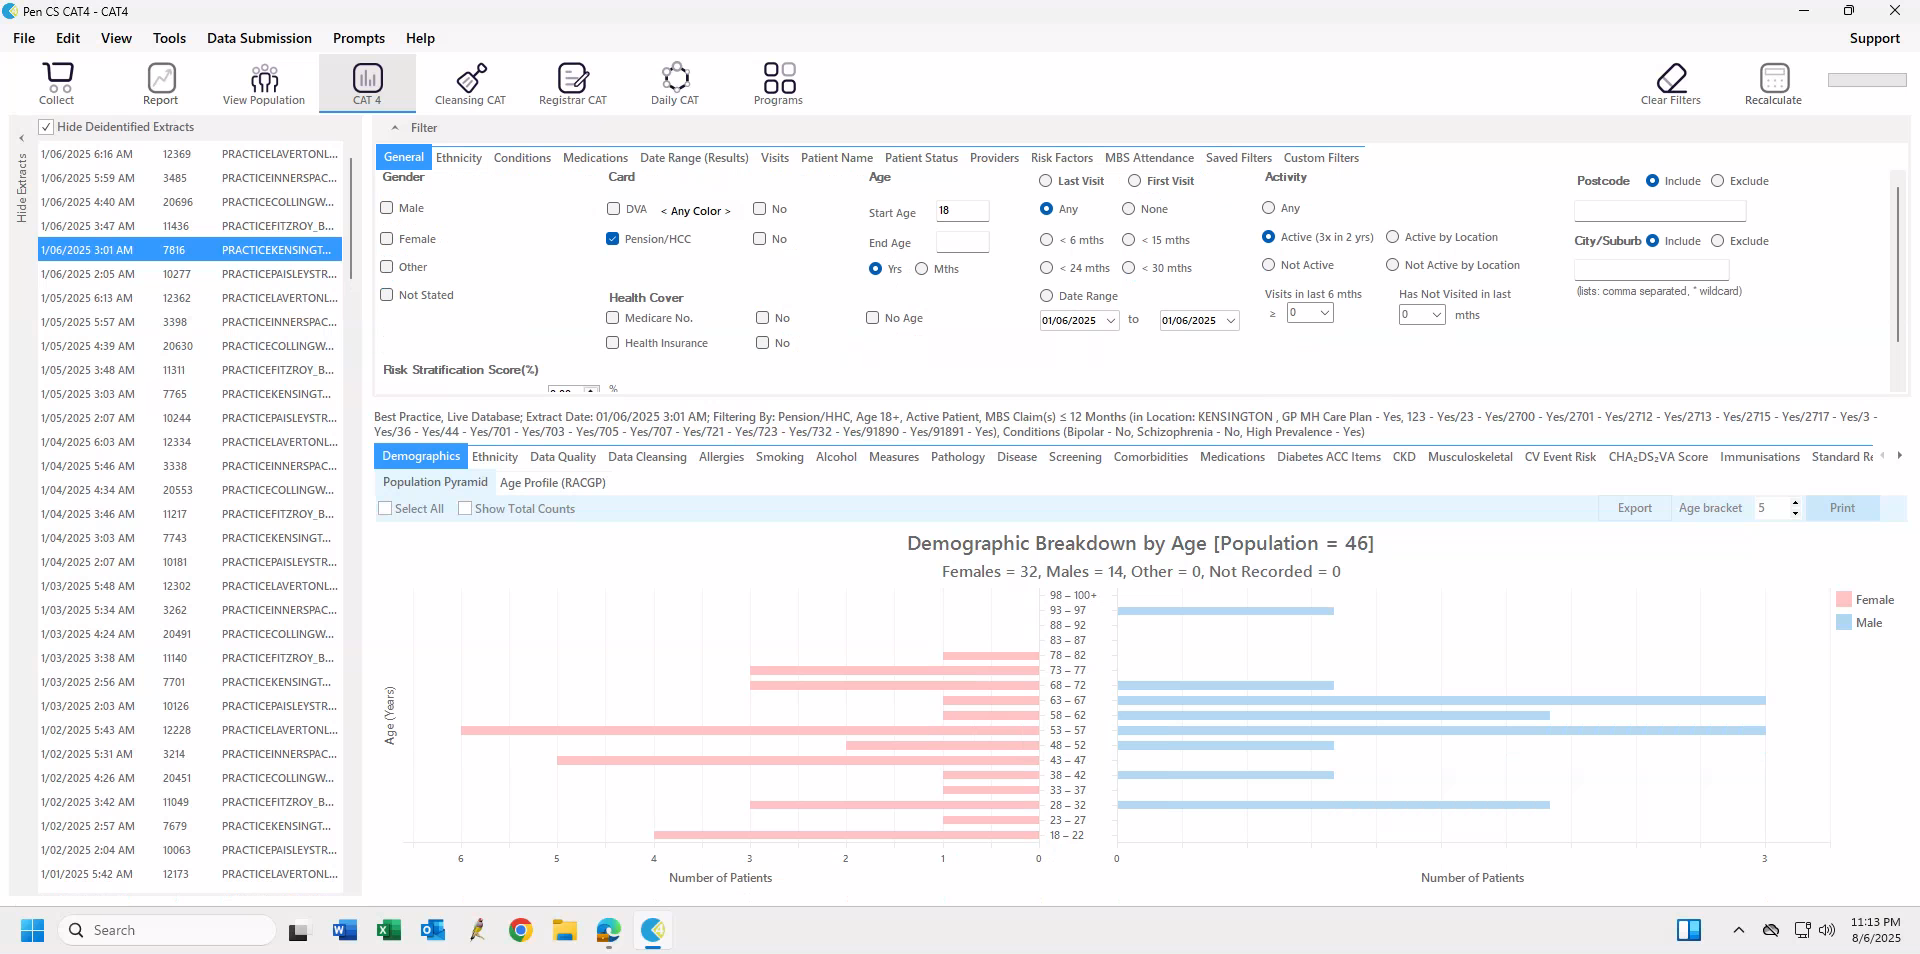
\includegraphics[keepaspectratio]{./images/PenCS.png}}

}

\caption{\label{figure-pencs}PenCS example, Kensington extract 1st June
2025 (note, not from 1st May 2025!)}

\end{figure}%

Patient high- or low- prevalence mental health condition status

\begin{itemize}
\tightlist
\item
  Using Filter `Conditions', sub-filter `Mental Health'

  \begin{itemize}
  \tightlist
  \item
    For patients with high-prevalence conditions

    \begin{itemize}
    \tightlist
    \item
      Set `High Prevalence' to yes (ticked).
    \item
      In this case, we are interested in patients with recorded
      low-prevalence conditions \emph{without} high-prevalence
      conditions. Set both the low-prevalence conditions (schizophrenia
      and bipolar) to `No' by ticking the `No' box for those two
      conditions.
    \end{itemize}
  \item
    For patients with low-prevalence conditions

    \begin{itemize}
    \tightlist
    \item
      Set `Low Prevalence' to yes (ticked).
    \item
      Many patients with low-prevalence conditions will also have
      high-prevalence mental health conditions. For this search, we are
      interested in the presence or absence of a low-prevalence mental
      health condition, regardless of the presence or absence of a
      high-prevalence condition.
    \end{itemize}
  \end{itemize}
\end{itemize}

Patient concession card status

\begin{itemize}
\tightlist
\item
  Using Filter `General'

  \begin{itemize}
  \tightlist
  \item
    Set `Card' to `Pension/HCC' or `No'
  \end{itemize}
\end{itemize}

Patient mental health treatment plan or other item numbers

\begin{itemize}
\tightlist
\item
  Using Filter `MBS Attendance'

  \begin{itemize}
  \tightlist
  \item
    For Mental health treatment plan (MHTP)

    \begin{itemize}
    \tightlist
    \item
      Set `GP MH Care Plan' to yes (ticked)
    \end{itemize}
  \item
    For Mental health consultation (MBS item `2713')

    \begin{itemize}
    \tightlist
    \item
      In `MBS Item Numbers' tick only item `2713'
    \end{itemize}
  \item
    For Chronic Disease management plans (MBS item `721')

    \begin{itemize}
    \tightlist
    \item
      In `MBS Item Numbers' tick only item `721'
    \end{itemize}
  \end{itemize}
\end{itemize}

\subsubsection{Supplementary tables}\label{supplementary-tables}

\begin{table}

\centering{

\begin{Shaded}
\begin{Highlighting}[]
\FunctionTok{table1}\NormalTok{(}
  \AttributeTok{x =} \SpecialCharTok{\textasciitilde{}}\NormalTok{ mh2713 }\SpecialCharTok{|}\NormalTok{ clinic,}
  \AttributeTok{data =}\NormalTok{ mh2713 }\SpecialCharTok{|\textgreater{}}
    \FunctionTok{mutate}\NormalTok{(}\AttributeTok{condition =} \FunctionTok{factor}\NormalTok{(condition, }\AttributeTok{label =} \FunctionTok{c}\NormalTok{(}\StringTok{"High{-}prevalence"}\NormalTok{, }\StringTok{"Low{-}prevalence"}\NormalTok{))),}
  \AttributeTok{overall =} \FunctionTok{c}\NormalTok{(}\AttributeTok{left =} \StringTok{"Total"}\NormalTok{)}
\NormalTok{) }\SpecialCharTok{|\textgreater{}}
  \FunctionTok{t1flex}\NormalTok{(}\AttributeTok{tablefn =} \StringTok{"flextable"}\NormalTok{, }\AttributeTok{cwidth =} \FloatTok{0.85}\NormalTok{) }\SpecialCharTok{|\textgreater{}}
  \FunctionTok{fontsize}\NormalTok{(}\AttributeTok{size =} \DecValTok{9}\NormalTok{, }\AttributeTok{part =} \StringTok{"all"}\NormalTok{) }\SpecialCharTok{|\textgreater{}}
  \FunctionTok{add\_footer\_lines}\NormalTok{(}\AttributeTok{value =} \FunctionTok{as\_paragraph}\NormalTok{(}\StringTok{"coHealth clinics, May 2025, \textquotesingle{}active\textquotesingle{} patients"}\NormalTok{))}
\end{Highlighting}
\end{Shaded}

\global\setlength{\Oldarrayrulewidth}{\arrayrulewidth}

\global\setlength{\Oldtabcolsep}{\tabcolsep}

\setlength{\tabcolsep}{2pt}

\renewcommand*{\arraystretch}{1.5}



\providecommand{\ascline}[3]{\noalign{\global\arrayrulewidth #1}\arrayrulecolor[HTML]{#2}\cline{#3}}

\begin{longtable*}[c]{|p{0.85in}|p{0.85in}|p{0.85in}|p{0.85in}|p{0.85in}|p{0.85in}|p{0.85in}}



\ascline{1.5pt}{666666}{1-7}

\multicolumn{1}{>{\raggedright}m{\dimexpr 0.85in+0\tabcolsep}}{\textcolor[HTML]{000000}{\fontsize{9}{9}\selectfont{\global\setmainfont{DejaVu Sans}{ }}}} & \multicolumn{1}{>{\centering}m{\dimexpr 0.85in+0\tabcolsep}}{\textcolor[HTML]{000000}{\fontsize{9}{9}\selectfont{\global\setmainfont{DejaVu Sans}{Total}}}\textcolor[HTML]{000000}{\fontsize{9}{9}\selectfont{\global\setmainfont{DejaVu Sans}{\linebreak }}}\textcolor[HTML]{000000}{\fontsize{9}{9}\selectfont{\global\setmainfont{DejaVu Sans}{(N=2544)}}}} & \multicolumn{1}{>{\centering}m{\dimexpr 0.85in+0\tabcolsep}}{\textcolor[HTML]{000000}{\fontsize{9}{9}\selectfont{\global\setmainfont{DejaVu Sans}{Collingwood}}}\textcolor[HTML]{000000}{\fontsize{9}{9}\selectfont{\global\setmainfont{DejaVu Sans}{\linebreak }}}\textcolor[HTML]{000000}{\fontsize{9}{9}\selectfont{\global\setmainfont{DejaVu Sans}{(N=527)}}}} & \multicolumn{1}{>{\centering}m{\dimexpr 0.85in+0\tabcolsep}}{\textcolor[HTML]{000000}{\fontsize{9}{9}\selectfont{\global\setmainfont{DejaVu Sans}{Fitzroy}}}\textcolor[HTML]{000000}{\fontsize{9}{9}\selectfont{\global\setmainfont{DejaVu Sans}{\linebreak }}}\textcolor[HTML]{000000}{\fontsize{9}{9}\selectfont{\global\setmainfont{DejaVu Sans}{(N=711)}}}} & \multicolumn{1}{>{\centering}m{\dimexpr 0.85in+0\tabcolsep}}{\textcolor[HTML]{000000}{\fontsize{9}{9}\selectfont{\global\setmainfont{DejaVu Sans}{Kensington}}}\textcolor[HTML]{000000}{\fontsize{9}{9}\selectfont{\global\setmainfont{DejaVu Sans}{\linebreak }}}\textcolor[HTML]{000000}{\fontsize{9}{9}\selectfont{\global\setmainfont{DejaVu Sans}{(N=450)}}}} & \multicolumn{1}{>{\centering}m{\dimexpr 0.85in+0\tabcolsep}}{\textcolor[HTML]{000000}{\fontsize{9}{9}\selectfont{\global\setmainfont{DejaVu Sans}{Laverton}}}\textcolor[HTML]{000000}{\fontsize{9}{9}\selectfont{\global\setmainfont{DejaVu Sans}{\linebreak }}}\textcolor[HTML]{000000}{\fontsize{9}{9}\selectfont{\global\setmainfont{DejaVu Sans}{(N=164)}}}} & \multicolumn{1}{>{\centering}m{\dimexpr 0.85in+0\tabcolsep}}{\textcolor[HTML]{000000}{\fontsize{9}{9}\selectfont{\global\setmainfont{DejaVu Sans}{Paisley}}}\textcolor[HTML]{000000}{\fontsize{9}{9}\selectfont{\global\setmainfont{DejaVu Sans}{\linebreak }}}\textcolor[HTML]{000000}{\fontsize{9}{9}\selectfont{\global\setmainfont{DejaVu Sans}{(N=692)}}}} \\

\ascline{1.5pt}{666666}{1-7}\endfirsthead 

\ascline{1.5pt}{666666}{1-7}

\multicolumn{1}{>{\raggedright}m{\dimexpr 0.85in+0\tabcolsep}}{\textcolor[HTML]{000000}{\fontsize{9}{9}\selectfont{\global\setmainfont{DejaVu Sans}{ }}}} & \multicolumn{1}{>{\centering}m{\dimexpr 0.85in+0\tabcolsep}}{\textcolor[HTML]{000000}{\fontsize{9}{9}\selectfont{\global\setmainfont{DejaVu Sans}{Total}}}\textcolor[HTML]{000000}{\fontsize{9}{9}\selectfont{\global\setmainfont{DejaVu Sans}{\linebreak }}}\textcolor[HTML]{000000}{\fontsize{9}{9}\selectfont{\global\setmainfont{DejaVu Sans}{(N=2544)}}}} & \multicolumn{1}{>{\centering}m{\dimexpr 0.85in+0\tabcolsep}}{\textcolor[HTML]{000000}{\fontsize{9}{9}\selectfont{\global\setmainfont{DejaVu Sans}{Collingwood}}}\textcolor[HTML]{000000}{\fontsize{9}{9}\selectfont{\global\setmainfont{DejaVu Sans}{\linebreak }}}\textcolor[HTML]{000000}{\fontsize{9}{9}\selectfont{\global\setmainfont{DejaVu Sans}{(N=527)}}}} & \multicolumn{1}{>{\centering}m{\dimexpr 0.85in+0\tabcolsep}}{\textcolor[HTML]{000000}{\fontsize{9}{9}\selectfont{\global\setmainfont{DejaVu Sans}{Fitzroy}}}\textcolor[HTML]{000000}{\fontsize{9}{9}\selectfont{\global\setmainfont{DejaVu Sans}{\linebreak }}}\textcolor[HTML]{000000}{\fontsize{9}{9}\selectfont{\global\setmainfont{DejaVu Sans}{(N=711)}}}} & \multicolumn{1}{>{\centering}m{\dimexpr 0.85in+0\tabcolsep}}{\textcolor[HTML]{000000}{\fontsize{9}{9}\selectfont{\global\setmainfont{DejaVu Sans}{Kensington}}}\textcolor[HTML]{000000}{\fontsize{9}{9}\selectfont{\global\setmainfont{DejaVu Sans}{\linebreak }}}\textcolor[HTML]{000000}{\fontsize{9}{9}\selectfont{\global\setmainfont{DejaVu Sans}{(N=450)}}}} & \multicolumn{1}{>{\centering}m{\dimexpr 0.85in+0\tabcolsep}}{\textcolor[HTML]{000000}{\fontsize{9}{9}\selectfont{\global\setmainfont{DejaVu Sans}{Laverton}}}\textcolor[HTML]{000000}{\fontsize{9}{9}\selectfont{\global\setmainfont{DejaVu Sans}{\linebreak }}}\textcolor[HTML]{000000}{\fontsize{9}{9}\selectfont{\global\setmainfont{DejaVu Sans}{(N=164)}}}} & \multicolumn{1}{>{\centering}m{\dimexpr 0.85in+0\tabcolsep}}{\textcolor[HTML]{000000}{\fontsize{9}{9}\selectfont{\global\setmainfont{DejaVu Sans}{Paisley}}}\textcolor[HTML]{000000}{\fontsize{9}{9}\selectfont{\global\setmainfont{DejaVu Sans}{\linebreak }}}\textcolor[HTML]{000000}{\fontsize{9}{9}\selectfont{\global\setmainfont{DejaVu Sans}{(N=692)}}}} \\

\ascline{1.5pt}{666666}{1-7}\endhead



\multicolumn{1}{>{\raggedright}m{\dimexpr 0.85in+0\tabcolsep}}{\textcolor[HTML]{000000}{\fontsize{9}{9}\selectfont{\global\setmainfont{DejaVu Sans}{\textbf{Mental\ Health\ GP\ Consult}}}}} & \multicolumn{1}{>{\centering}m{\dimexpr 0.85in+0\tabcolsep}}{\textcolor[HTML]{000000}{\fontsize{9}{9}\selectfont{\global\setmainfont{DejaVu Sans}{}}}} & \multicolumn{1}{>{\centering}m{\dimexpr 0.85in+0\tabcolsep}}{\textcolor[HTML]{000000}{\fontsize{9}{9}\selectfont{\global\setmainfont{DejaVu Sans}{}}}} & \multicolumn{1}{>{\centering}m{\dimexpr 0.85in+0\tabcolsep}}{\textcolor[HTML]{000000}{\fontsize{9}{9}\selectfont{\global\setmainfont{DejaVu Sans}{}}}} & \multicolumn{1}{>{\centering}m{\dimexpr 0.85in+0\tabcolsep}}{\textcolor[HTML]{000000}{\fontsize{9}{9}\selectfont{\global\setmainfont{DejaVu Sans}{}}}} & \multicolumn{1}{>{\centering}m{\dimexpr 0.85in+0\tabcolsep}}{\textcolor[HTML]{000000}{\fontsize{9}{9}\selectfont{\global\setmainfont{DejaVu Sans}{}}}} & \multicolumn{1}{>{\centering}m{\dimexpr 0.85in+0\tabcolsep}}{\textcolor[HTML]{000000}{\fontsize{9}{9}\selectfont{\global\setmainfont{DejaVu Sans}{}}}} \\





\multicolumn{1}{>{\raggedright}m{\dimexpr 0.85in+0\tabcolsep}}{\textcolor[HTML]{000000}{\fontsize{9}{9}\selectfont{\global\setmainfont{DejaVu Sans}{  Yes}}}} & \multicolumn{1}{>{\centering}m{\dimexpr 0.85in+0\tabcolsep}}{\textcolor[HTML]{000000}{\fontsize{9}{9}\selectfont{\global\setmainfont{DejaVu Sans}{189\ (7.4\%)}}}} & \multicolumn{1}{>{\centering}m{\dimexpr 0.85in+0\tabcolsep}}{\textcolor[HTML]{000000}{\fontsize{9}{9}\selectfont{\global\setmainfont{DejaVu Sans}{31\ (5.9\%)}}}} & \multicolumn{1}{>{\centering}m{\dimexpr 0.85in+0\tabcolsep}}{\textcolor[HTML]{000000}{\fontsize{9}{9}\selectfont{\global\setmainfont{DejaVu Sans}{45\ (6.3\%)}}}} & \multicolumn{1}{>{\centering}m{\dimexpr 0.85in+0\tabcolsep}}{\textcolor[HTML]{000000}{\fontsize{9}{9}\selectfont{\global\setmainfont{DejaVu Sans}{24\ (5.3\%)}}}} & \multicolumn{1}{>{\centering}m{\dimexpr 0.85in+0\tabcolsep}}{\textcolor[HTML]{000000}{\fontsize{9}{9}\selectfont{\global\setmainfont{DejaVu Sans}{23\ (14.0\%)}}}} & \multicolumn{1}{>{\centering}m{\dimexpr 0.85in+0\tabcolsep}}{\textcolor[HTML]{000000}{\fontsize{9}{9}\selectfont{\global\setmainfont{DejaVu Sans}{66\ (9.5\%)}}}} \\





\multicolumn{1}{>{\raggedright}m{\dimexpr 0.85in+0\tabcolsep}}{\textcolor[HTML]{000000}{\fontsize{9}{9}\selectfont{\global\setmainfont{DejaVu Sans}{  No}}}} & \multicolumn{1}{>{\centering}m{\dimexpr 0.85in+0\tabcolsep}}{\textcolor[HTML]{000000}{\fontsize{9}{9}\selectfont{\global\setmainfont{DejaVu Sans}{2355\ (92.6\%)}}}} & \multicolumn{1}{>{\centering}m{\dimexpr 0.85in+0\tabcolsep}}{\textcolor[HTML]{000000}{\fontsize{9}{9}\selectfont{\global\setmainfont{DejaVu Sans}{496\ (94.1\%)}}}} & \multicolumn{1}{>{\centering}m{\dimexpr 0.85in+0\tabcolsep}}{\textcolor[HTML]{000000}{\fontsize{9}{9}\selectfont{\global\setmainfont{DejaVu Sans}{666\ (93.7\%)}}}} & \multicolumn{1}{>{\centering}m{\dimexpr 0.85in+0\tabcolsep}}{\textcolor[HTML]{000000}{\fontsize{9}{9}\selectfont{\global\setmainfont{DejaVu Sans}{426\ (94.7\%)}}}} & \multicolumn{1}{>{\centering}m{\dimexpr 0.85in+0\tabcolsep}}{\textcolor[HTML]{000000}{\fontsize{9}{9}\selectfont{\global\setmainfont{DejaVu Sans}{141\ (86.0\%)}}}} & \multicolumn{1}{>{\centering}m{\dimexpr 0.85in+0\tabcolsep}}{\textcolor[HTML]{000000}{\fontsize{9}{9}\selectfont{\global\setmainfont{DejaVu Sans}{626\ (90.5\%)}}}} \\

\ascline{1.5pt}{666666}{1-7}



\multicolumn{7}{>{\raggedright}m{\dimexpr 5.95in+12\tabcolsep}}{\textcolor[HTML]{000000}{\fontsize{11}{11}\selectfont{\global\setmainfont{DejaVu Sans}{coHealth\ clinics,\ May\ 2025,\ 'active'\ patients}}}} \\





\end{longtable*}



\arrayrulecolor[HTML]{000000}

\global\setlength{\arrayrulewidth}{\Oldarrayrulewidth}

\global\setlength{\tabcolsep}{\Oldtabcolsep}

\renewcommand*{\arraystretch}{1}

}

\caption{\label{table-mh2713_by_clinic}Mental health GP consultations
(MBS 2713) claimed in the previous twelve months, by clinic site.}

\end{table}%

\begin{table}

\centering{

\begin{Shaded}
\begin{Highlighting}[]
\FunctionTok{table1}\NormalTok{(}
  \AttributeTok{x =} \SpecialCharTok{\textasciitilde{}}\NormalTok{ gpmp }\SpecialCharTok{|}\NormalTok{ clinic,}
  \AttributeTok{data =}\NormalTok{ gpmp }\SpecialCharTok{|\textgreater{}}
    \FunctionTok{mutate}\NormalTok{(}\AttributeTok{condition =} \FunctionTok{factor}\NormalTok{(condition, }\AttributeTok{label =} \FunctionTok{c}\NormalTok{(}\StringTok{"High{-}prevalence"}\NormalTok{, }\StringTok{"Low{-}prevalence"}\NormalTok{))),}
  \AttributeTok{overall =} \FunctionTok{c}\NormalTok{(}\AttributeTok{left =} \StringTok{"Total"}\NormalTok{),}
\NormalTok{) }\SpecialCharTok{|\textgreater{}}
  \FunctionTok{t1flex}\NormalTok{(}\AttributeTok{tablefn =} \StringTok{"flextable"}\NormalTok{, }\AttributeTok{cwidth =} \FloatTok{0.85}\NormalTok{) }\SpecialCharTok{|\textgreater{}}
  \FunctionTok{fontsize}\NormalTok{(}\AttributeTok{size =} \DecValTok{9}\NormalTok{, }\AttributeTok{part =} \StringTok{"all"}\NormalTok{) }\SpecialCharTok{|\textgreater{}}
  \FunctionTok{add\_footer\_lines}\NormalTok{(}\AttributeTok{value =} \FunctionTok{as\_paragraph}\NormalTok{(}\StringTok{"coHealth clinics, May 2025, \textquotesingle{}active\textquotesingle{} patients"}\NormalTok{))}
\end{Highlighting}
\end{Shaded}

\global\setlength{\Oldarrayrulewidth}{\arrayrulewidth}

\global\setlength{\Oldtabcolsep}{\tabcolsep}

\setlength{\tabcolsep}{2pt}

\renewcommand*{\arraystretch}{1.5}



\providecommand{\ascline}[3]{\noalign{\global\arrayrulewidth #1}\arrayrulecolor[HTML]{#2}\cline{#3}}

\begin{longtable*}[c]{|p{0.85in}|p{0.85in}|p{0.85in}|p{0.85in}|p{0.85in}|p{0.85in}|p{0.85in}}



\ascline{1.5pt}{666666}{1-7}

\multicolumn{1}{>{\raggedright}m{\dimexpr 0.85in+0\tabcolsep}}{\textcolor[HTML]{000000}{\fontsize{9}{9}\selectfont{\global\setmainfont{DejaVu Sans}{ }}}} & \multicolumn{1}{>{\centering}m{\dimexpr 0.85in+0\tabcolsep}}{\textcolor[HTML]{000000}{\fontsize{9}{9}\selectfont{\global\setmainfont{DejaVu Sans}{Total}}}\textcolor[HTML]{000000}{\fontsize{9}{9}\selectfont{\global\setmainfont{DejaVu Sans}{\linebreak }}}\textcolor[HTML]{000000}{\fontsize{9}{9}\selectfont{\global\setmainfont{DejaVu Sans}{(N=2544)}}}} & \multicolumn{1}{>{\centering}m{\dimexpr 0.85in+0\tabcolsep}}{\textcolor[HTML]{000000}{\fontsize{9}{9}\selectfont{\global\setmainfont{DejaVu Sans}{Collingwood}}}\textcolor[HTML]{000000}{\fontsize{9}{9}\selectfont{\global\setmainfont{DejaVu Sans}{\linebreak }}}\textcolor[HTML]{000000}{\fontsize{9}{9}\selectfont{\global\setmainfont{DejaVu Sans}{(N=527)}}}} & \multicolumn{1}{>{\centering}m{\dimexpr 0.85in+0\tabcolsep}}{\textcolor[HTML]{000000}{\fontsize{9}{9}\selectfont{\global\setmainfont{DejaVu Sans}{Fitzroy}}}\textcolor[HTML]{000000}{\fontsize{9}{9}\selectfont{\global\setmainfont{DejaVu Sans}{\linebreak }}}\textcolor[HTML]{000000}{\fontsize{9}{9}\selectfont{\global\setmainfont{DejaVu Sans}{(N=711)}}}} & \multicolumn{1}{>{\centering}m{\dimexpr 0.85in+0\tabcolsep}}{\textcolor[HTML]{000000}{\fontsize{9}{9}\selectfont{\global\setmainfont{DejaVu Sans}{Kensington}}}\textcolor[HTML]{000000}{\fontsize{9}{9}\selectfont{\global\setmainfont{DejaVu Sans}{\linebreak }}}\textcolor[HTML]{000000}{\fontsize{9}{9}\selectfont{\global\setmainfont{DejaVu Sans}{(N=450)}}}} & \multicolumn{1}{>{\centering}m{\dimexpr 0.85in+0\tabcolsep}}{\textcolor[HTML]{000000}{\fontsize{9}{9}\selectfont{\global\setmainfont{DejaVu Sans}{Laverton}}}\textcolor[HTML]{000000}{\fontsize{9}{9}\selectfont{\global\setmainfont{DejaVu Sans}{\linebreak }}}\textcolor[HTML]{000000}{\fontsize{9}{9}\selectfont{\global\setmainfont{DejaVu Sans}{(N=164)}}}} & \multicolumn{1}{>{\centering}m{\dimexpr 0.85in+0\tabcolsep}}{\textcolor[HTML]{000000}{\fontsize{9}{9}\selectfont{\global\setmainfont{DejaVu Sans}{Paisley}}}\textcolor[HTML]{000000}{\fontsize{9}{9}\selectfont{\global\setmainfont{DejaVu Sans}{\linebreak }}}\textcolor[HTML]{000000}{\fontsize{9}{9}\selectfont{\global\setmainfont{DejaVu Sans}{(N=692)}}}} \\

\ascline{1.5pt}{666666}{1-7}\endfirsthead 

\ascline{1.5pt}{666666}{1-7}

\multicolumn{1}{>{\raggedright}m{\dimexpr 0.85in+0\tabcolsep}}{\textcolor[HTML]{000000}{\fontsize{9}{9}\selectfont{\global\setmainfont{DejaVu Sans}{ }}}} & \multicolumn{1}{>{\centering}m{\dimexpr 0.85in+0\tabcolsep}}{\textcolor[HTML]{000000}{\fontsize{9}{9}\selectfont{\global\setmainfont{DejaVu Sans}{Total}}}\textcolor[HTML]{000000}{\fontsize{9}{9}\selectfont{\global\setmainfont{DejaVu Sans}{\linebreak }}}\textcolor[HTML]{000000}{\fontsize{9}{9}\selectfont{\global\setmainfont{DejaVu Sans}{(N=2544)}}}} & \multicolumn{1}{>{\centering}m{\dimexpr 0.85in+0\tabcolsep}}{\textcolor[HTML]{000000}{\fontsize{9}{9}\selectfont{\global\setmainfont{DejaVu Sans}{Collingwood}}}\textcolor[HTML]{000000}{\fontsize{9}{9}\selectfont{\global\setmainfont{DejaVu Sans}{\linebreak }}}\textcolor[HTML]{000000}{\fontsize{9}{9}\selectfont{\global\setmainfont{DejaVu Sans}{(N=527)}}}} & \multicolumn{1}{>{\centering}m{\dimexpr 0.85in+0\tabcolsep}}{\textcolor[HTML]{000000}{\fontsize{9}{9}\selectfont{\global\setmainfont{DejaVu Sans}{Fitzroy}}}\textcolor[HTML]{000000}{\fontsize{9}{9}\selectfont{\global\setmainfont{DejaVu Sans}{\linebreak }}}\textcolor[HTML]{000000}{\fontsize{9}{9}\selectfont{\global\setmainfont{DejaVu Sans}{(N=711)}}}} & \multicolumn{1}{>{\centering}m{\dimexpr 0.85in+0\tabcolsep}}{\textcolor[HTML]{000000}{\fontsize{9}{9}\selectfont{\global\setmainfont{DejaVu Sans}{Kensington}}}\textcolor[HTML]{000000}{\fontsize{9}{9}\selectfont{\global\setmainfont{DejaVu Sans}{\linebreak }}}\textcolor[HTML]{000000}{\fontsize{9}{9}\selectfont{\global\setmainfont{DejaVu Sans}{(N=450)}}}} & \multicolumn{1}{>{\centering}m{\dimexpr 0.85in+0\tabcolsep}}{\textcolor[HTML]{000000}{\fontsize{9}{9}\selectfont{\global\setmainfont{DejaVu Sans}{Laverton}}}\textcolor[HTML]{000000}{\fontsize{9}{9}\selectfont{\global\setmainfont{DejaVu Sans}{\linebreak }}}\textcolor[HTML]{000000}{\fontsize{9}{9}\selectfont{\global\setmainfont{DejaVu Sans}{(N=164)}}}} & \multicolumn{1}{>{\centering}m{\dimexpr 0.85in+0\tabcolsep}}{\textcolor[HTML]{000000}{\fontsize{9}{9}\selectfont{\global\setmainfont{DejaVu Sans}{Paisley}}}\textcolor[HTML]{000000}{\fontsize{9}{9}\selectfont{\global\setmainfont{DejaVu Sans}{\linebreak }}}\textcolor[HTML]{000000}{\fontsize{9}{9}\selectfont{\global\setmainfont{DejaVu Sans}{(N=692)}}}} \\

\ascline{1.5pt}{666666}{1-7}\endhead



\multicolumn{1}{>{\raggedright}m{\dimexpr 0.85in+0\tabcolsep}}{\textcolor[HTML]{000000}{\fontsize{9}{9}\selectfont{\global\setmainfont{DejaVu Sans}{\textbf{Chronic\ Disease\ Management\ Plan}}}}} & \multicolumn{1}{>{\centering}m{\dimexpr 0.85in+0\tabcolsep}}{\textcolor[HTML]{000000}{\fontsize{9}{9}\selectfont{\global\setmainfont{DejaVu Sans}{}}}} & \multicolumn{1}{>{\centering}m{\dimexpr 0.85in+0\tabcolsep}}{\textcolor[HTML]{000000}{\fontsize{9}{9}\selectfont{\global\setmainfont{DejaVu Sans}{}}}} & \multicolumn{1}{>{\centering}m{\dimexpr 0.85in+0\tabcolsep}}{\textcolor[HTML]{000000}{\fontsize{9}{9}\selectfont{\global\setmainfont{DejaVu Sans}{}}}} & \multicolumn{1}{>{\centering}m{\dimexpr 0.85in+0\tabcolsep}}{\textcolor[HTML]{000000}{\fontsize{9}{9}\selectfont{\global\setmainfont{DejaVu Sans}{}}}} & \multicolumn{1}{>{\centering}m{\dimexpr 0.85in+0\tabcolsep}}{\textcolor[HTML]{000000}{\fontsize{9}{9}\selectfont{\global\setmainfont{DejaVu Sans}{}}}} & \multicolumn{1}{>{\centering}m{\dimexpr 0.85in+0\tabcolsep}}{\textcolor[HTML]{000000}{\fontsize{9}{9}\selectfont{\global\setmainfont{DejaVu Sans}{}}}} \\





\multicolumn{1}{>{\raggedright}m{\dimexpr 0.85in+0\tabcolsep}}{\textcolor[HTML]{000000}{\fontsize{9}{9}\selectfont{\global\setmainfont{DejaVu Sans}{  Yes}}}} & \multicolumn{1}{>{\centering}m{\dimexpr 0.85in+0\tabcolsep}}{\textcolor[HTML]{000000}{\fontsize{9}{9}\selectfont{\global\setmainfont{DejaVu Sans}{756\ (29.7\%)}}}} & \multicolumn{1}{>{\centering}m{\dimexpr 0.85in+0\tabcolsep}}{\textcolor[HTML]{000000}{\fontsize{9}{9}\selectfont{\global\setmainfont{DejaVu Sans}{126\ (23.9\%)}}}} & \multicolumn{1}{>{\centering}m{\dimexpr 0.85in+0\tabcolsep}}{\textcolor[HTML]{000000}{\fontsize{9}{9}\selectfont{\global\setmainfont{DejaVu Sans}{147\ (20.7\%)}}}} & \multicolumn{1}{>{\centering}m{\dimexpr 0.85in+0\tabcolsep}}{\textcolor[HTML]{000000}{\fontsize{9}{9}\selectfont{\global\setmainfont{DejaVu Sans}{164\ (36.4\%)}}}} & \multicolumn{1}{>{\centering}m{\dimexpr 0.85in+0\tabcolsep}}{\textcolor[HTML]{000000}{\fontsize{9}{9}\selectfont{\global\setmainfont{DejaVu Sans}{67\ (40.9\%)}}}} & \multicolumn{1}{>{\centering}m{\dimexpr 0.85in+0\tabcolsep}}{\textcolor[HTML]{000000}{\fontsize{9}{9}\selectfont{\global\setmainfont{DejaVu Sans}{252\ (36.4\%)}}}} \\





\multicolumn{1}{>{\raggedright}m{\dimexpr 0.85in+0\tabcolsep}}{\textcolor[HTML]{000000}{\fontsize{9}{9}\selectfont{\global\setmainfont{DejaVu Sans}{  No}}}} & \multicolumn{1}{>{\centering}m{\dimexpr 0.85in+0\tabcolsep}}{\textcolor[HTML]{000000}{\fontsize{9}{9}\selectfont{\global\setmainfont{DejaVu Sans}{1788\ (70.3\%)}}}} & \multicolumn{1}{>{\centering}m{\dimexpr 0.85in+0\tabcolsep}}{\textcolor[HTML]{000000}{\fontsize{9}{9}\selectfont{\global\setmainfont{DejaVu Sans}{401\ (76.1\%)}}}} & \multicolumn{1}{>{\centering}m{\dimexpr 0.85in+0\tabcolsep}}{\textcolor[HTML]{000000}{\fontsize{9}{9}\selectfont{\global\setmainfont{DejaVu Sans}{564\ (79.3\%)}}}} & \multicolumn{1}{>{\centering}m{\dimexpr 0.85in+0\tabcolsep}}{\textcolor[HTML]{000000}{\fontsize{9}{9}\selectfont{\global\setmainfont{DejaVu Sans}{286\ (63.6\%)}}}} & \multicolumn{1}{>{\centering}m{\dimexpr 0.85in+0\tabcolsep}}{\textcolor[HTML]{000000}{\fontsize{9}{9}\selectfont{\global\setmainfont{DejaVu Sans}{97\ (59.1\%)}}}} & \multicolumn{1}{>{\centering}m{\dimexpr 0.85in+0\tabcolsep}}{\textcolor[HTML]{000000}{\fontsize{9}{9}\selectfont{\global\setmainfont{DejaVu Sans}{440\ (63.6\%)}}}} \\

\ascline{1.5pt}{666666}{1-7}



\multicolumn{7}{>{\raggedright}m{\dimexpr 5.95in+12\tabcolsep}}{\textcolor[HTML]{000000}{\fontsize{11}{11}\selectfont{\global\setmainfont{DejaVu Sans}{coHealth\ clinics,\ May\ 2025,\ 'active'\ patients}}}} \\





\end{longtable*}



\arrayrulecolor[HTML]{000000}

\global\setlength{\arrayrulewidth}{\Oldarrayrulewidth}

\global\setlength{\tabcolsep}{\Oldtabcolsep}

\renewcommand*{\arraystretch}{1}

}

\caption{\label{table-gpmp_by_clinic}GP chronic disease management plans
(MBS item 721) claimed in the previous twelve months, by clinic site.}

\end{table}%




\end{document}
